
\documentclass[11pt]{article}

\usepackage[utf8]{inputenc}
\usepackage[T1]{fontenc}
\usepackage{amsmath,amssymb}
\usepackage{mathtools}
\usepackage{booktabs}
\usepackage{longtable}
\usepackage{array}
\usepackage[margin=1in]{geometry}
\usepackage{siunitx}
\usepackage{graphicx}
\usepackage[hidelinks]{hyperref}
\usepackage{xcolor}
\usepackage{enumitem}
\usepackage{amsfonts}
\usepackage{textcomp}

% siunitx v2 spellings used by some model sections
\providecommand{\celsius}{\degreeCelsius}
\ProvideDocumentCommand\squared{}{\tothe{2}}
\ProvideDocumentCommand\cubed{}{\tothe{3}}

\sisetup{per-mode=symbol}

% ---------- macros, matching the companion model report ----------
\newcommand{\md}{\ensuremath{\dot m}}
\newcommand{\mdp}{\ensuremath{\dot m_{\mathrm{pro}}}}
\newcommand{\mdr}{\ensuremath{\dot m_{\mathrm{reg}}}}
\newcommand{\mdv}{\ensuremath{\dot m_{\mathrm{vent}}}}
\newcommand{\mdw}{\ensuremath{\dot m_{w}}}
\newcommand{\UA}{\ensuremath{U\!A}}
\newcommand{\hfg}{\ensuremath{h_{\mathrm{fg}}}}
\newcommand{\patm}{\ensuremath{p_{\mathrm{atm}}}}
\newcommand{\psat}{\ensuremath{p_{\mathrm{sat}}}}
\newcommand{\RH}{\ensuremath{\mathrm{RH}}}
\newcommand{\degC}{\ensuremath{^{\circ}\mathrm{C}}}
\newcommand{\qs}{\ensuremath{q_{s}}}
\newcommand{\ql}{\ensuremath{q_{l}}}

\title{\textbf{Master Architecture of the DBHE-Driven\\
Heating, Cooling and Dehumidification Plant}\\[6pt]
\large Streams, Junctions, Valve Network, Operating Modes,\\
Load Interface, and Verification Protocol\\[4pt]
\normalsize (Generated from model version 10.6, stamped 2026-08-01 09:35 BRT)}
\author{Craft \& Hawkins Department of Petroleum Engineering\\
Louisiana State University}
\date{\today}

\begin{document}
\maketitle

\begin{abstract}
This document specifies the \emph{master architecture} of the surface plant
driven by a closed-loop Deep Borehole Heat Exchanger formed from a repurposed
legacy oil-and-gas well. Where the companion model report derives the governing
equations of each component, this report defines the \emph{topology}: which
streams exist, where they join and split, which valve or damper controls each
branch, and which subset of components is active in each operating mode.
The architecture is deliberately a superset. It contains every component the
plant could need across the full plane of sensible and latent loads, and a
given operating mode is obtained by activating a subset of branches rather
than by rebuilding the plant. Section~\ref{sec:modes} enumerates the resulting
modes; Section~\ref{sec:status} records which components are implemented in the
code and which are pending.

Part~II gives the mathematical model of every component, written against the
source rather than from memory, together with a specification for the four
components the architecture contains but the code does not yet.

The report is generated, not transcribed. Part~I's tables and the version
history are extracted at build time from the notebook, the frozen regression
fixtures and the parametric sweep archives; the configuration constants quoted
in Part~II's prose are frozen in a fixture of their own and the build fails if
any of them moves. The document is regenerated whenever the model version
changes.
\end{abstract}

\tableofcontents
\newpage

\part{The plant: architecture, modes, and the resource that limits them}

% ==========================================================================
\section{Scope, and how this document stays current}
% ==========================================================================

\subsection{What is specified here}

The plant comprises five fluid circuits: the geothermal water loop, a chilled
water loop, a cooling-tower water loop, the process (building supply) air
stream, and the scavenging (regeneration) air stream. The master architecture
is the union of all flow paths among them. It is not a single machine but a
family: each operating mode activates a subset of the branches, and the
inactive branches are present but idle.

Two consequences follow, and they shape the whole study. First, the number of
distinct plants is finite and small once the valves and dampers are treated as
two-position devices rather than continuously modulating ones. Second, the
question ``which plant should be built'' becomes ``which subset of the master
architecture serves the load quadrants that actually occur, using the water
temperature the well can actually deliver over the design life''. That is the
question Sections~\ref{sec:modes} and \ref{sec:resource} address.

\subsection{Generation, not transcription}

This report is emitted by \verb|report/build_report.py| in the model
repository. The build step reads:

\begin{itemize}[nosep]
  \item the notebook, for the version stamp and the configuration constants;
  \item \verb|verification/reference/v*_baseline.json|, the frozen per-version
        results recorded by the regression harness;
  \item the parametric sweep archives, for the resource-feasibility tables.
\end{itemize}

When the model advances to the next version the report is rebuilt and
republished, and the version history in Section~\ref{sec:history} gains a row
by itself.

\paragraph{Where the guarantee is weaker, and what protects it there.}
No number in Part~I is typed by hand; a Part~I statement that contradicts the
code is a defect in the build script, not a stale paragraph. Part~II cannot
work that way. Its model sections quote constants inside prose and inside
derivations --- \emph{the damper floor is} \num{0.05}, \emph{the coil is sized
at} \SI{3000}{\watt\per\kelvin} \emph{per} \si{\kilogram\per\second} --- and
templating prose at that density would make it unreadable. Those numbers are
typed, so they can rot.

The guard is a configuration fixture. \verb|report/check_config.py| snapshots
every scalar assignment in the configuration cell, and every subsequent build
compares the live notebook against that snapshot. If a constant moves, the
build stops and names the symbol, so the affected prose is re-read and the
fixture re-frozen deliberately rather than by accident. This is the same
discipline the model itself uses --- freeze a reference, never overwrite it
silently --- applied to the document. It does not prove the prose is right; it
guarantees that a change in the code cannot pass unnoticed.

% ==========================================================================
\section{Nomenclature convention}
% ==========================================================================

State labels follow a two- or three-letter convention. The first subscript
letter identifies the stream: \emph{w} for geothermal water, \emph{c} for
chilled water, \emph{p} for process air, \emph{r} for scavenging
(regeneration) air, \emph{t} for cooling-tower water. Subsequent letters
identify the station. Valves on water circuits are $v_{A}\ldots v_{H}$;
dampers on air circuits are $d_{pA}\ldots d_{pI}$ for the process stream and
$d_{rA}, d_{rB}$ for the scavenging stream.

\begin{longtable}{@{}llp{0.52\textwidth}@{}}
\toprule
\textbf{Symbol} & \textbf{Circuit} & \textbf{Station} \\
\midrule
\endhead
$T_{\mathrm{in}}$   & water & injection into the annulus \\
$T_{\mathrm{ret}}$  & water & production from the tubing \\
$T_{\mathrm{wr}}$   & water & after the $v_F$ well-bypass rejoins the production stream \\
$T_{\mathrm{wa}}$   & water & accumulator outlet \\
$T_{\mathrm{wg}}$   & water & absorption-generator outlet \\
$T_{\mathrm{wma}}$  & water & generator-skip branch merged with the $v_B$ accumulator bypass \\
$T_{\mathrm{wmg}}$  & water & $T_{\mathrm{wg}}$ tempered by $T_{\mathrm{wma}}$ through $v_D$ \\
$T_{\mathrm{wx}}$   & water & regeneration heat-exchanger outlet \\
$T_{\mathrm{wmx}}$  & water & after the $v_H$ remainder blends back; returns to the pump \\
\midrule
$T_{pc}, w_{pc}$    & process air & building comfort state (return) \\
$T_{pmc}, w_{pmc}$  & process air & mixed state entering the supply fan \\
$T_{pd}, w_{pd}$    & process air & desiccant-wheel process outlet \\
$T_{pmo}, w_{pmo}$  & process air & after fork~1 remerges, entering fork~2 \\
$T_{pi}, w_{pi}$    & process air & building supply \\
$T_{ea}, \RH_{ea}$  & process air & building exhaust \\
\midrule
$T_{rm}, w_{rm}$    & scavenging air & mixed state entering the scavenging fan \\
$T_{ri}, w_{ri}$    & scavenging air & regeneration-coil inlet \\
$T_{ro}, w_{ro}$    & scavenging air & regeneration-coil outlet, wheel inlet \\
$T_{rd}, w_{rd}$    & scavenging air & wheel regeneration outlet, vented \\
\bottomrule
\end{longtable}

% ==========================================================================
\section{The five circuits}
% ==========================================================================

\begin{figure}[p]
\centering
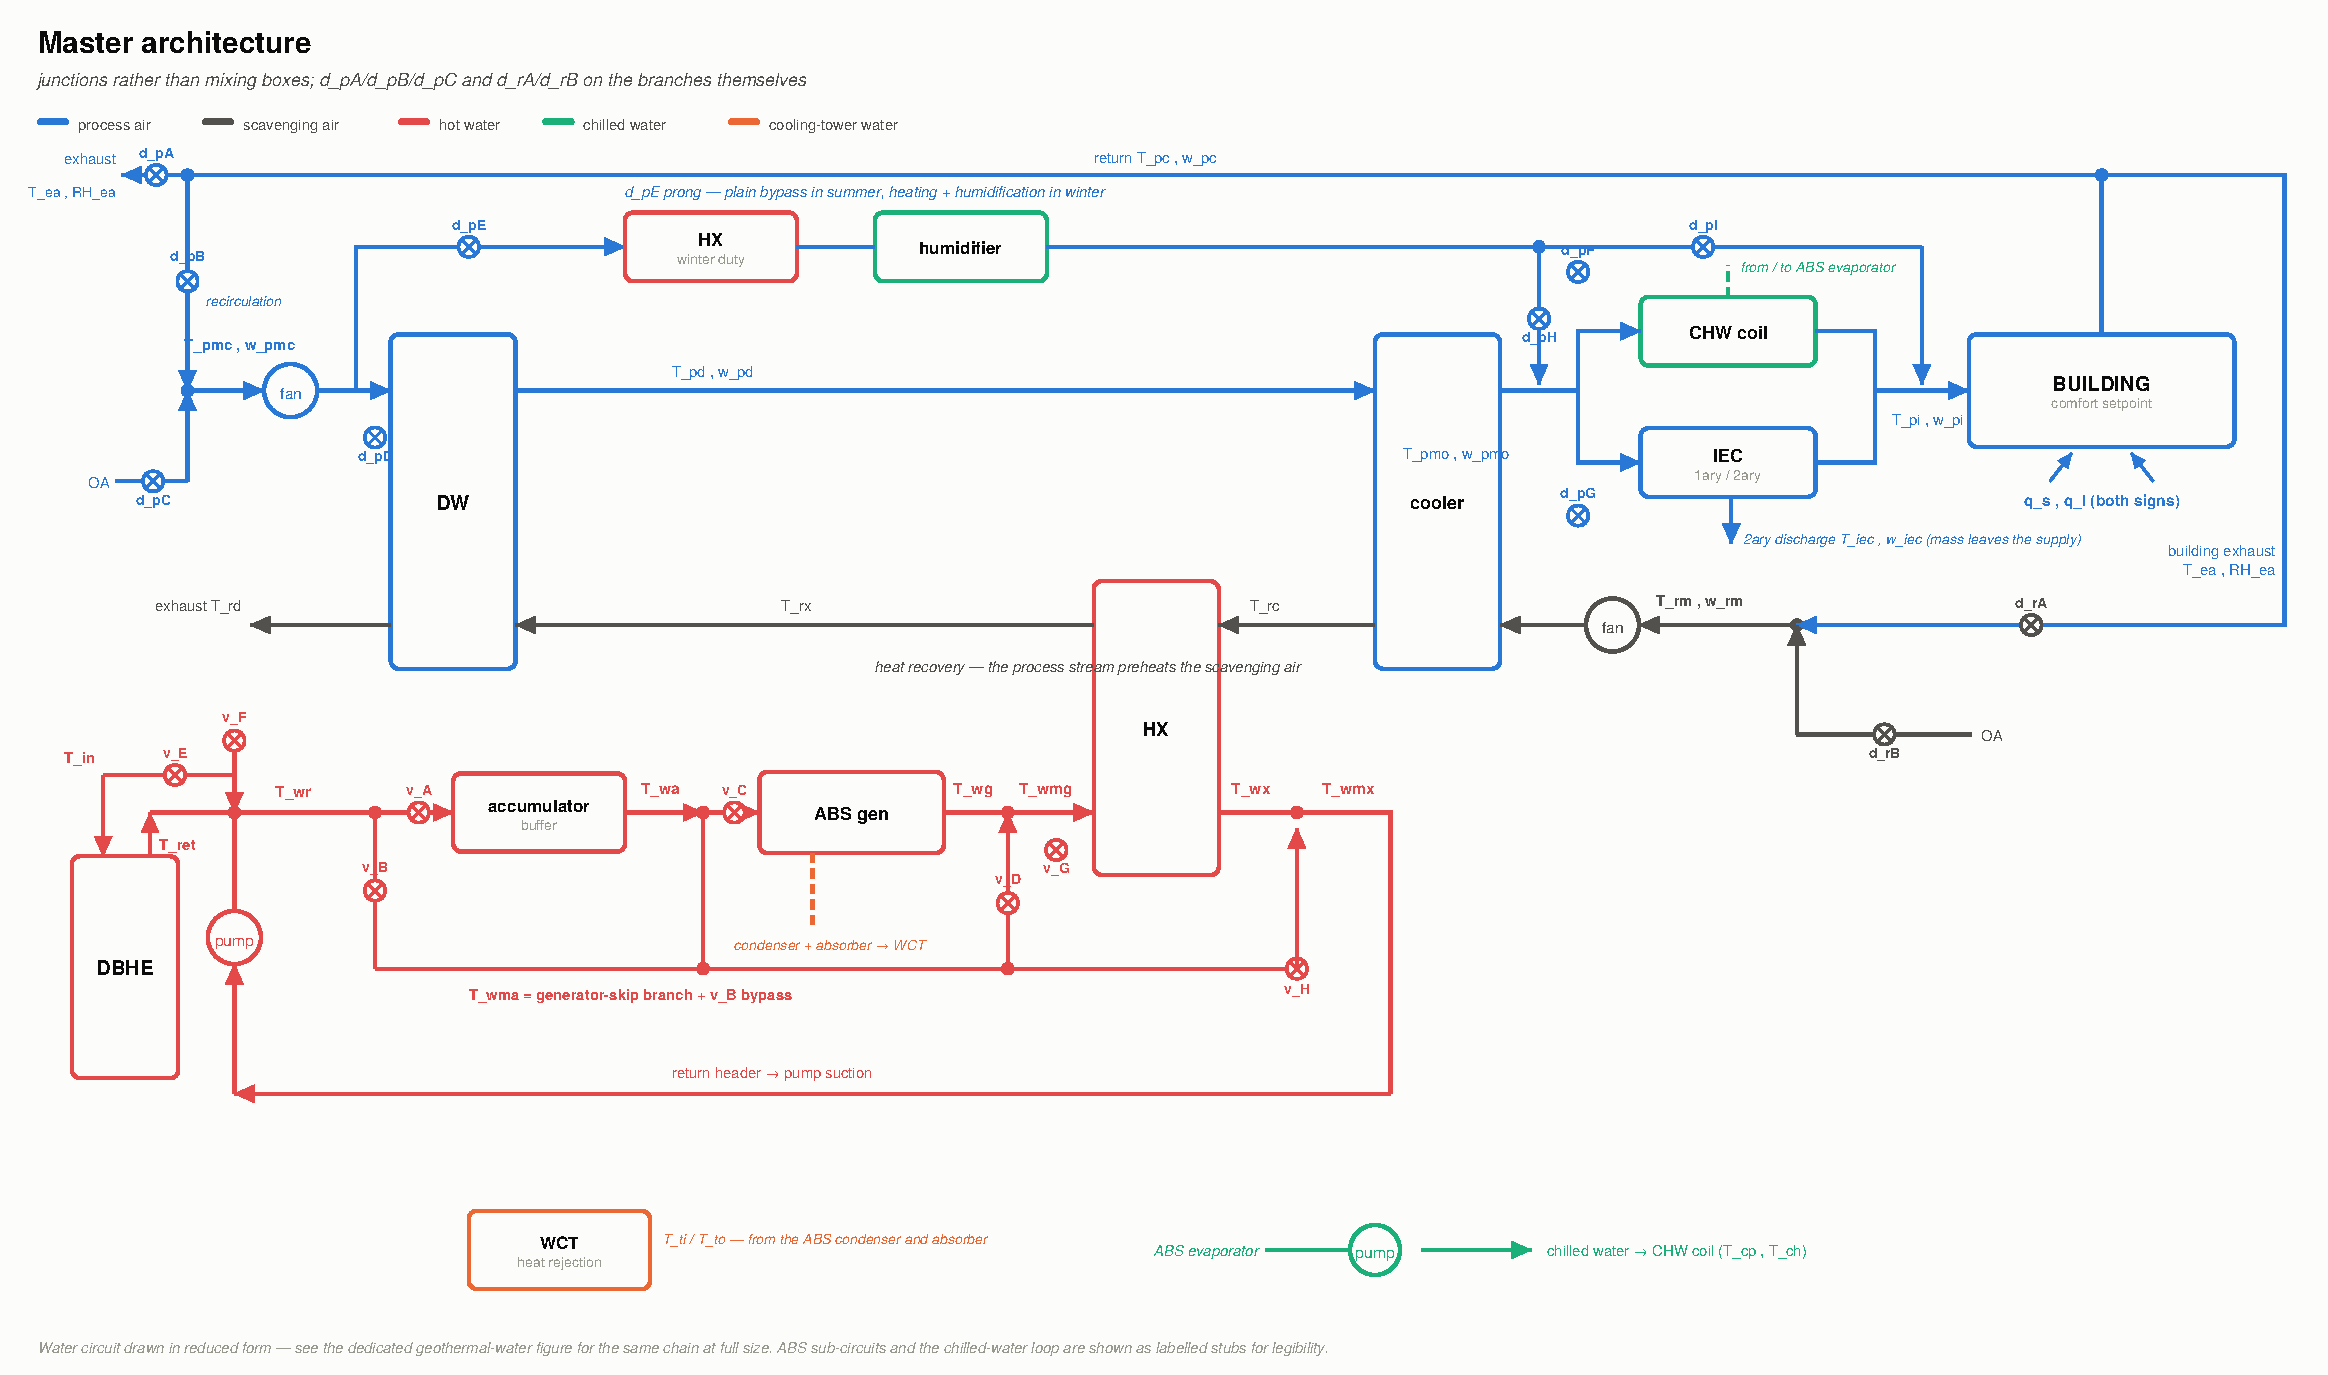
\includegraphics[width=\textwidth]{figures/master_architecture.pdf}
\caption{Master architecture. Every component the plant could need across the
full load plane is present; an operating mode is a subset of active branches,
not a different machine.}\label{fig:master}
\end{figure}

\subsection{Geothermal water}

\begin{figure}[p]
\centering
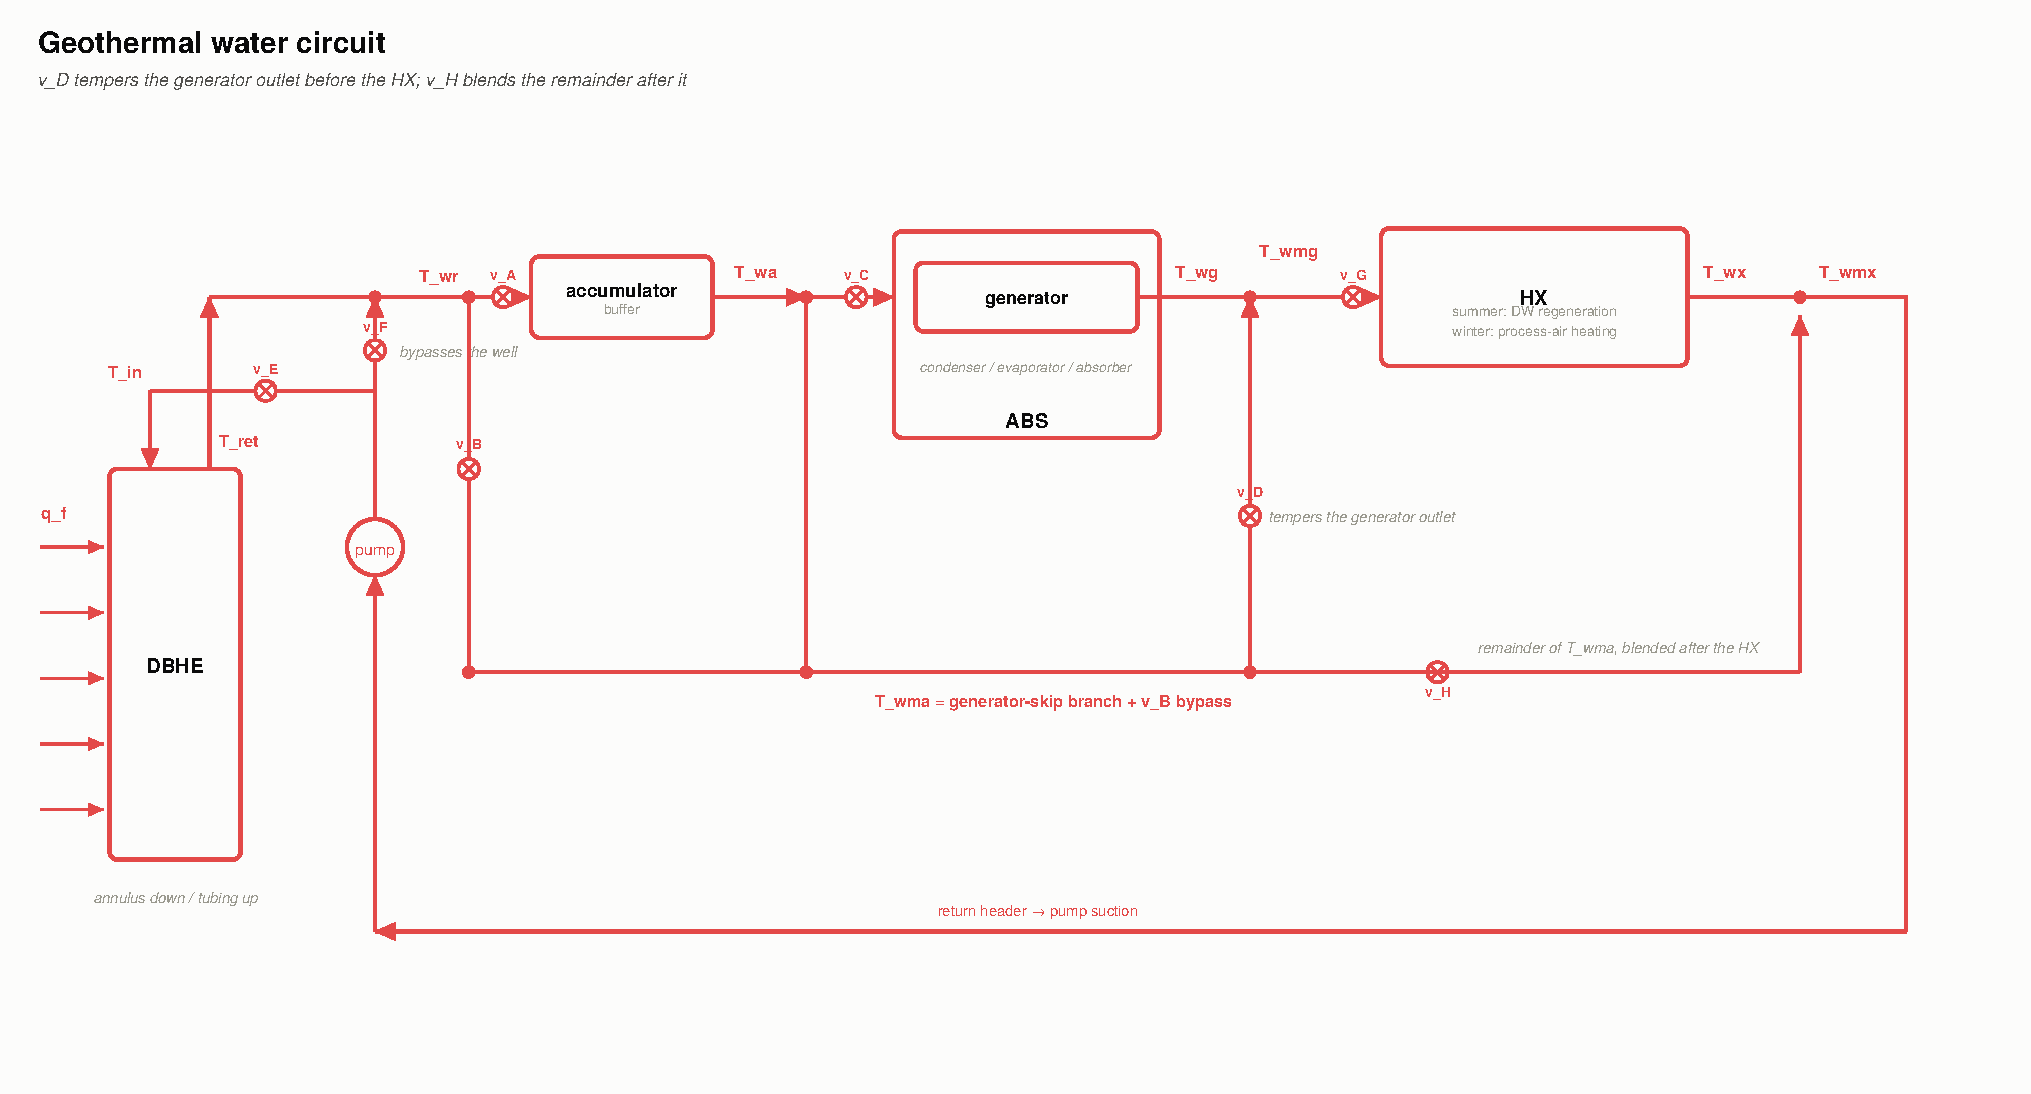
\includegraphics[width=\textwidth]{figures/water_circuit.pdf}
\caption{Geothermal water circuit. $v_E$/$v_F$ decouple loop flow from well
flow; $v_A$/$v_B$ gate the accumulator; $v_C$ gates the absorption generator;
$v_D$ raises the coil inlet, while $v_G$/$v_H$ throttle the coil
duty.}\label{fig:water}
\end{figure}

The water circuit is a closed loop with four decision points. Reading from the
pump:

\begin{enumerate}[nosep]
  \item \textbf{$v_E$ / $v_F$ --- well bifurcation.} $v_E$ sends flow down the
        annulus; $v_F$ bypasses the well entirely and rejoins the production
        stream. The mixed state is $T_{\mathrm{wr}}$. This decouples the loop
        flow from the well flow, so the surface plant can be run at a flow the
        subsurface would not tolerate, and vice versa.
  \item \textbf{$v_A$ / $v_B$ --- accumulator.} $v_A$ charges or discharges the
        thermal store; $v_B$ bypasses it. The accumulator is a buffer, not a
        topology choice: its state varies through the day within any mode.
  \item \textbf{$v_C$ --- absorption generator.} The branch that skips the
        generator merges with the $v_B$ bypass to form $T_{\mathrm{wma}}$.
  \item \textbf{$v_D$, then $v_G$ / $v_H$.} $v_D$ blends $T_{\mathrm{wma}}$ into
        the generator outlet $T_{\mathrm{wg}}$, raising the regeneration-coil
        inlet to $T_{\mathrm{wmg}}$. $v_G$ passes that stream through the coil;
        $v_H$ carries the remainder of $T_{\mathrm{wma}}$ around the coil to
        blend with the coil outlet $T_{\mathrm{wx}}$, giving
        $T_{\mathrm{wmx}}$.
\end{enumerate}

The pairing of $v_D$ and $v_G$ deserves emphasis because the two are easily
confused. \textbf{$v_D$ raises} the coil inlet temperature: it can only blend
\emph{hotter} bypass water into a generator outlet that the chiller has cooled.
\textbf{$v_G$ throttles}: reducing the share of flow through the coil lowers
the coil duty, hence the regeneration air temperature $T_{\mathrm{ro}}$, hence
the drying the wheel performs. When the wheel must be turned \emph{down},
$v_G$ is the control and $v_D$ is not.

\subsection{Process air}

\begin{equation*}
\text{mix} \;\to\; \text{fan} \;\to\;
\underbrace{\Big\{ d_{pD} \to \mathrm{DW} \to \mathrm{cooler}
\;\Big|\; d_{pE} \to \mathrm{HX_{winter}} \to \mathrm{humidifier} \Big\}}_{\text{fork 1}}
\;\to\; T_{pmo} \;\to\;
\underbrace{\Big\{ d_{pF} \to \mathrm{CHW} \;\Big|\; d_{pG} \to \mathrm{IEC} \Big\}}_{\text{fork 2}}
\;\to\; T_{pi}
\end{equation*}

The building return stream bifurcates at a node: $d_{pA}$ exhausts,
$d_{pB}$ recirculates, and the recirculated air joins outdoor air admitted
through $d_{pC}$ at a mixing junction whose state is $T_{pmc}, w_{pmc}$.

Fork~1 selects between conditioning (wheel followed by the recuperative
cooler) and the alternative prong that carries the winter heating coil and the
humidifier. The $d_{pE}$ prong terminates in two dampers: $d_{pH}$ returns it
to $T_{pmo}$, upstream of fork~2, which is the summer bypass; $d_{pI}$ carries
it past fork~2 directly into the supply duct, which is the winter path. Fork~2
is a genuine parallel pair --- chilled-water coil \emph{or} indirect
evaporative cooler, never both --- rejoining at the supply state
$T_{pi}, w_{pi}$.

Fork~2 needs no third ``neither'' prong: with no chilled water circulating and
no evaporative water supplied, air passes either branch at nothing but a
pressure drop.

\subsection{Scavenging air}

\begin{equation*}
\text{mix}\big(d_{rA}\,\text{building exhaust} + d_{rB}\,\text{outdoor air}\big)
\to \text{fan} \to \text{cooler} \to \mathrm{HX} \to \mathrm{DW} \to \text{vented}
\end{equation*}

Two features of this circuit carry more weight than their simplicity suggests.

First, the scavenging stream passes through the \textbf{cooler before the
regeneration coil}, so the process stream's rejected heat preheats it and the
coil has less lifting to do. The cooler is therefore a recuperator between the
two air streams, not a heat rejection device.

Second, the mixing junction draws on \textbf{building exhaust and outdoor
air}, and never on the wheel's own regeneration outlet. Recirculating the
wheel exhaust returns its desorbed moisture to its own inlet, which collapses
the relative-humidity difference the wheel drives on. The code did exactly
that until v10.5; correcting it nearly tripled moisture removal.

A physical bound constrains the mix. The building can only exhaust what it
admits as fresh air, so the exhaust available to the scavenging loop is
$\mdv = \SI{10.00}{\kilogram\per\second}$ against a scavenging demand
of $\mdr = \SI{23.52}{\kilogram\per\second}$. The building-exhaust
fraction is therefore capped at $0.425$ and the balance made up with
outdoor air.

\subsection{Chilled water and heat rejection}

The absorption chiller is a single indivisible subsystem with its
chilled-water distribution: a generator fed by geothermal water, an evaporator
serving the chilled-water coil in the process stream, and a condenser and
absorber rejecting to a wet cooling tower. A chiller with nowhere to send
chilled water is not a configuration, so \textbf{ABS and CHW are one switch,
not two}.

% ==========================================================================
\section{The load interface}
% ==========================================================================

The plant sees the building only through a steady, well-mixed pair of balances.
With $\qs > 0$ meaning cooling is required and $\mdw > 0$ meaning
dehumidification is required,

\begin{align}
\qs   &= \mdp\, c_p \,(T_{pc} - T_{pi}), \label{eq:sens}\\
\mdw  &= \mdp\, (w_{pc} - w_{pi}). \label{eq:lat}
\end{align}

Two equations, three unknowns $(\mdp, T_{pi}, w_{pi})$. \textbf{Exactly one
closure must be supplied}, and which one is a design decision rather than a
physical fact:

\begin{itemize}[nosep]
  \item give $\mdp$ --- constant volume; the supply state follows;
  \item give $\Delta T_{\mathrm{sup}} = T_{pc}-T_{pi}$ --- variable volume;
        the flow follows.
\end{itemize}

Dividing \eqref{eq:sens} by \eqref{eq:lat} eliminates the flow:

\begin{equation}
\frac{T_{pc}-T_{pi}}{w_{pc}-w_{pi}} = \frac{\qs}{\mdw}\,\frac{1}{c_p}.
\end{equation}

The load \emph{ratio} alone fixes the direction of the room condition line on
the psychrometric chart; the closure fixes how far along that line the supply
state sits. This is the classical construction, and it is why the interface
needs exactly one more piece of information and no more.

\paragraph{Latent load is carried as a moisture rate, not as a power.}
Expressing $\ql$ in kilowatts requires choosing $\hfg$, and inverting
\eqref{eq:lat} requires choosing it again. If the two choices differ --- and
values between 2450 and \SI{2501}{\kilo\joule\per\kilogram} are all in common
use --- $w_{pi}$ is wrong by about 2\%\ with nothing on screen to show it. The
interface therefore takes $\mdw$ in \si{\kilogram\per\second} and offers a
convenience wrapper that converts from kilowatts with an explicit $\hfg$.

\paragraph{The closure in the hatchery case is derived, not given.}
The supply flow is set by a design sensible load carried at a prescribed
supply depression, floored by the forced ventilation requirement:

\begin{equation}
\mdp = \max\!\left(\frac{Q_{s,\mathrm{design}}}{c_p\,\Delta T_{\mathrm{sup,design}}},\;
\mdv\right)
= \max\!\left(\SI{33.60}{\kilogram\per\second},\;
\SI{10.00}{\kilogram\per\second}\right)
= \SI{33.60}{\kilogram\per\second}.
\end{equation}

The depression rule binds. Its consequence reaches much further than fan
sizing: a supply depression of only $\SI{3}{\kelvin}$ demands a large
airflow, and a large airflow needs only a very small humidity difference to
carry the same latent load. The wheel is not underperforming in this plant ---
it is barely being asked to work.

% ==========================================================================
\section{Operating modes}\label{sec:modes}
% ==========================================================================

\subsection{Naming}

Load quadrants are named by the \emph{processes they require}, from the sign
pair $(\operatorname{sgn}\qs, \operatorname{sgn}\ql)$: cooling or heating,
combined with dehumidification or humidification. Seasonal names were
considered and rejected: they are climate-relative, since hot-and-dry is the
only summer in a semi-arid region, and setpoint-relative, since the quadrant
boundaries sit at the comfort state rather than at some neutral condition.

The sensible heat ratio cannot classify the quadrants on its own. Two negative
loads give a positive ratio, indistinguishable from two positive ones. The
sign pair is the primitive; the ratio describes position \emph{within} a
quadrant.

\subsection{Two axes: quadrant and tier}

\begin{figure}[p]
\centering
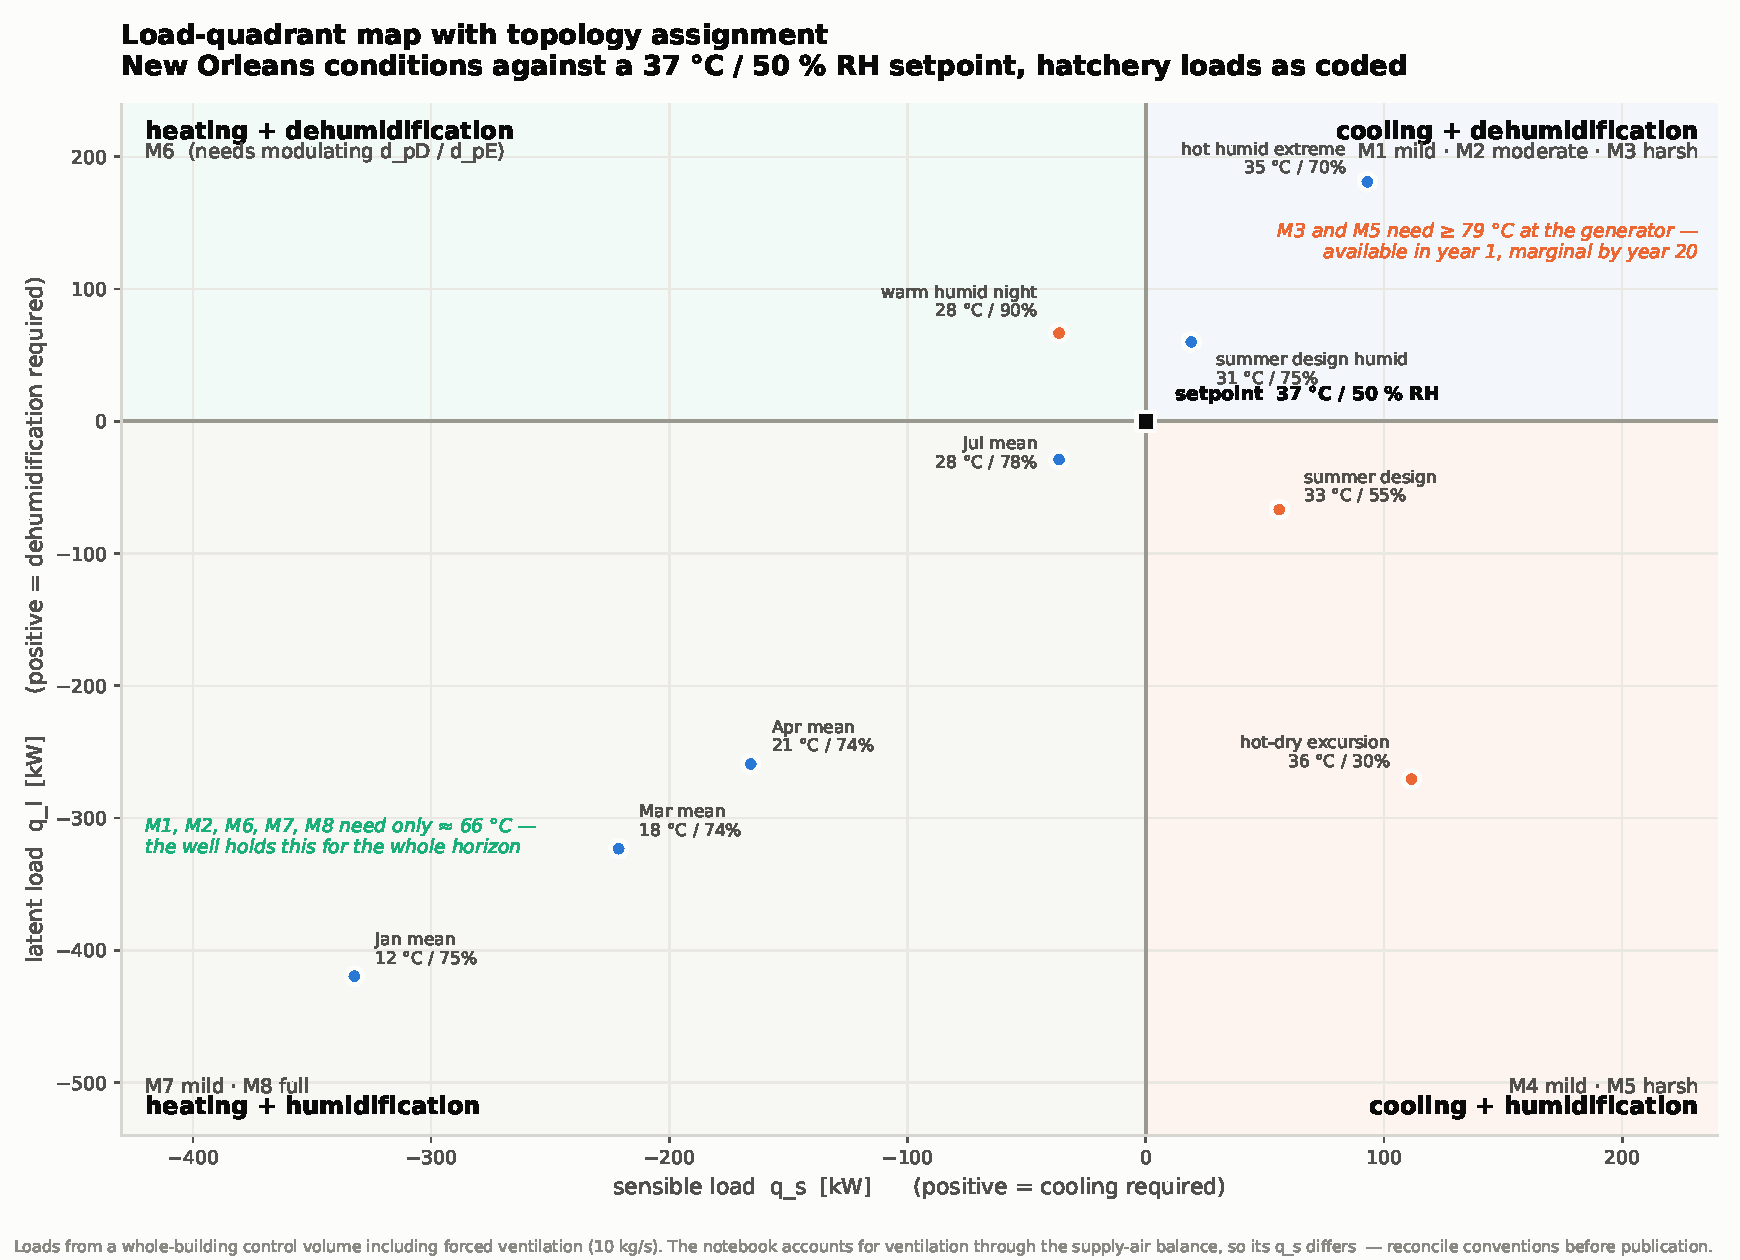
\includegraphics[width=\textwidth]{figures/quadrant_map.pdf}
\caption{The load plane. Quadrants are named by the processes they require;
the tier within a quadrant is set by load magnitude against what the well can
deliver.}\label{fig:qmap}
\end{figure}

\begin{figure}[p]
\centering
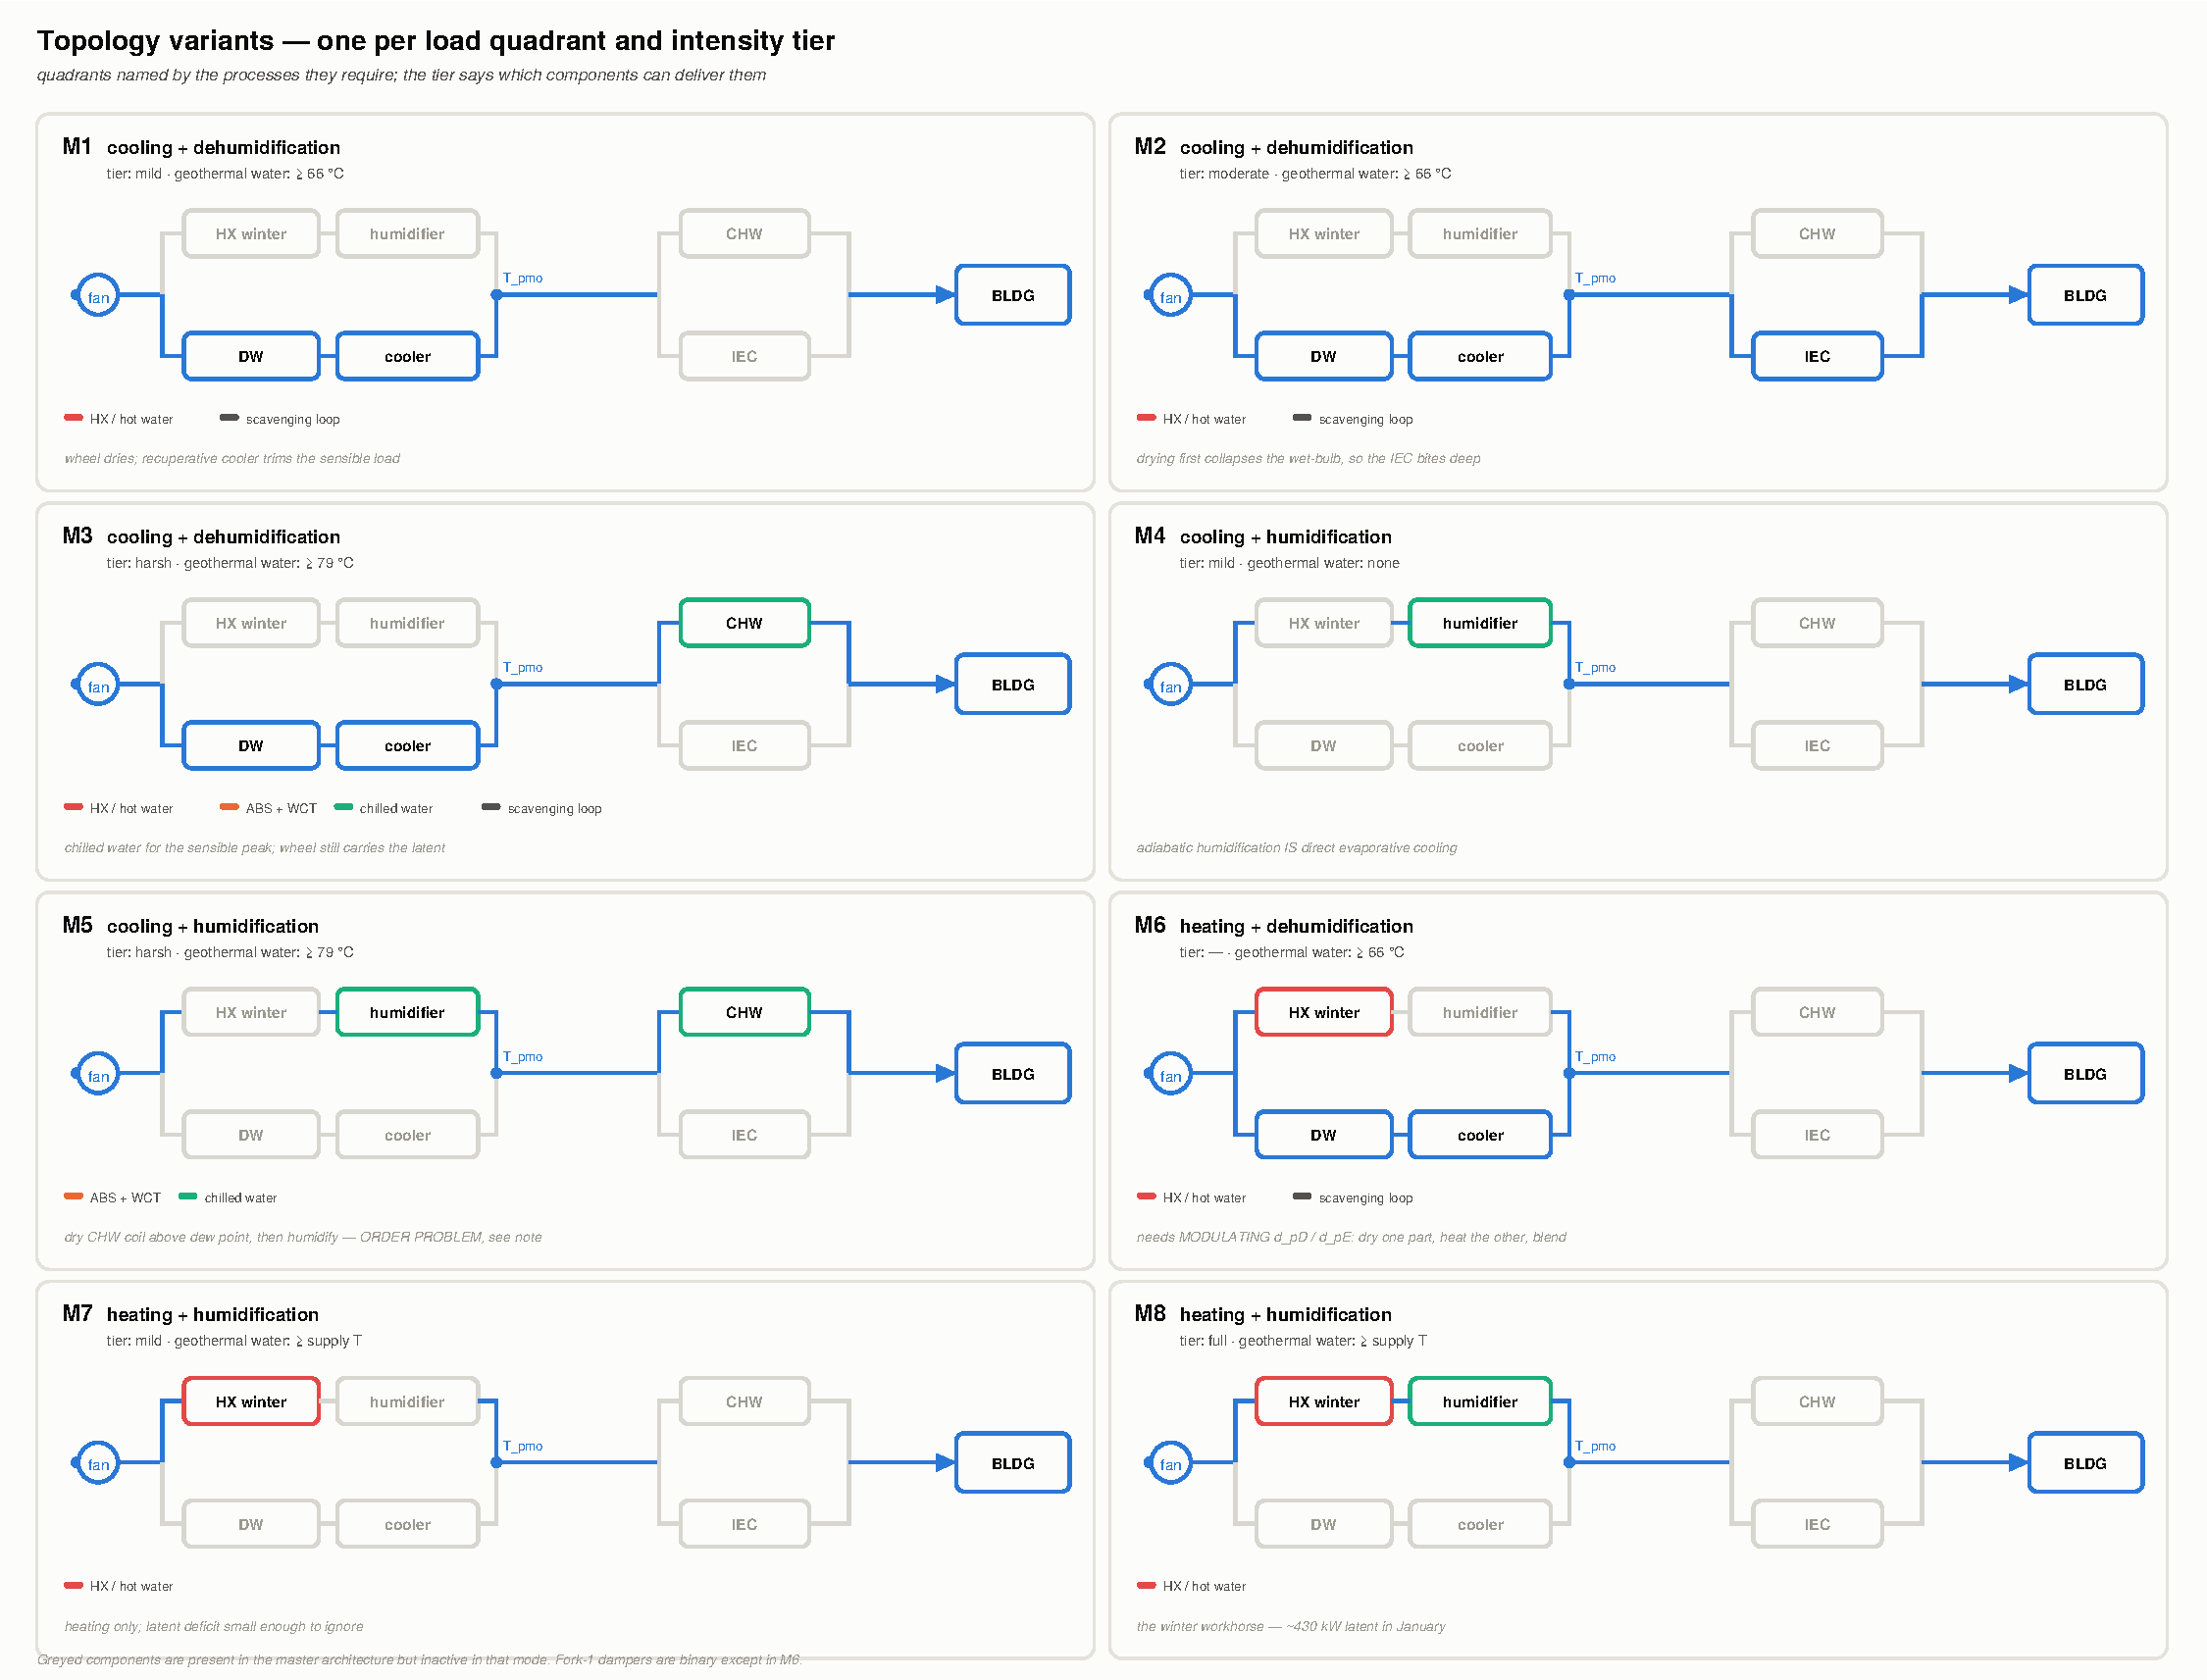
\includegraphics[width=\textwidth]{figures/topology_variants.pdf}
\caption{Topology variants. Each card shows the branches active in one mode;
inactive branches remain installed but idle.}\label{fig:topo}
\end{figure}

The quadrant selects which processes are needed. The load \emph{magnitude}
selects which components can deliver them. The resulting mode set is:

\begin{longtable}{@{}llp{0.36\textwidth}l@{}}
\toprule
\textbf{Mode} & \textbf{Quadrant} & \textbf{Active components} & \textbf{Water required} \\
\midrule
\endhead
M1 & cooling + dehumidification & DW, cooler & $\geq \SI{66}{\degreeCelsius}$ \\
M2 & cooling + dehumidification & DW, cooler, IEC & $\geq \SI{66}{\degreeCelsius}$ \\
M3 & cooling + dehumidification & DW, cooler, ABS + CHW & $\geq \SI{79}{\degreeCelsius}$ \\
M4 & cooling + humidification & humidifier alone (adiabatic saturation \emph{is} direct evaporative cooling) & none \\
M5 & cooling + humidification & ABS + CHW, humidifier & $\geq \SI{79}{\degreeCelsius}$ \\
M6 & heating + dehumidification & DW, cooler and winter coil, \emph{blended} & $\geq \SI{66}{\degreeCelsius}$ \\
M7 & heating + humidification & winter coil & $\geq$ supply $T$ \\
M8 & heating + humidification & winter coil, humidifier & $\geq$ supply $T$ \\
\bottomrule
\end{longtable}

Three of these carry conditions worth stating explicitly.

\textbf{M6 is the only mode requiring modulating dampers.} Dehumidification
and heating sit on parallel prongs of fork~1, so the quadrant is reached by
drying part of the flow, heating the rest, and blending at $T_{pmo}$. Every
other mode is satisfied by two-position devices.

\textbf{M5 has an unresolved ordering problem.} The humidifier sits on the
$d_{pE}$ prong, upstream of the chilled-water coil in fork~2, so the air is
humidified before it is cooled and may reach saturation. Cooling and then
humidifying is the correct sequence, and the architecture does not currently
provide it.

\textbf{M7 and M8 route through prong D with the wheel stopped.} Air passes a
stationary wheel at nothing but a pressure drop, which turns the cooler into an
exhaust-to-supply recuperator at no capital cost --- see
Section~\ref{sec:winter}.

% ==========================================================================
\section{The resource constraint}\label{sec:resource}
% ==========================================================================

\subsection{Temperature: which tiers the well can serve}

Only M3 and M5 require the \SI{79}{\degreeCelsius} minimum at the absorption
generator. Every other mode needs approximately \SI{66}{\degreeCelsius} for
wheel regeneration, which the well holds for the whole design life at almost
any flow. The serviceable region of the load plane therefore \emph{shrinks
with reservoir depletion, and it shrinks from the cooling corner first}.

From the archived parametric sweep, year-20 conditions:

\begin{longtable}{@{}rrrrrrc@{}}
\toprule
$L$ [\si{\metre}] & BHT [\degC] & $q$ [\si{\cubic\metre\per\hour}] &
$T_{\mathrm{ret}}$ [\degC] & $T_{\mathrm{wa}}$ [\degC] &
$Q_{\mathrm{well}}$ [\si{\kilo\watt}] & generator viable \\
\midrule
\endhead
4000 & 144.0 & 3 & 79.8 & 71.4 & 130 & no \\
4000 & 144.0 & 4 & 78.7 & 72.2 & 168 & no \\
4000 & 144.0 & 5 & 76.4 & 71.4 & 197 & no \\
4000 & 144.0 & 6 & 73.8 & 69.8 & 220 & no \\
4000 & 144.0 & 8 & 69.1 & 66.3 & 251 & no \\
4000 & 144.0 & 10 & 65.4 & 63.4 & 270 & no \\
4500 & 159.5 & 3 & 86.5 & 77.0 & 149 & no \\
4500 & 159.5 & 4 & 86.4 & 78.9 & 198 & yes \\
4500 & 159.5 & 5 & 84.5 & 78.5 & 237 & yes \\
4500 & 159.5 & 6 & 82.0 & 77.2 & 267 & no \\
4500 & 159.5 & 8 & 77.0 & 73.7 & 309 & no \\
4500 & 159.5 & 10 & 72.8 & 70.4 & 336 & no \\
4677 & 165.0 & 3 & 88.8 & 78.8 & 156 & yes \\
4677 & 165.0 & 4 & 89.1 & 81.2 & 208 & yes \\
4677 & 165.0 & 5 & 87.3 & 81.1 & 251 & yes \\
4677 & 165.0 & 6 & 84.9 & 79.8 & 283 & yes \\
4677 & 165.0 & 8 & 79.8 & 76.3 & 331 & no \\
4677 & 165.0 & 10 & 75.6 & 73.0 & 360 & no \\

\bottomrule
\end{longtable}

\subsection{Capacity: the flow squeeze}

Raising loop flow raises the generator duty but lowers the water temperature,
and the two requirements are not satisfied at the same operating point. Using a
design generator drop of \SI{10}{\kelvin} and a maximum of \SI{18}{\kelvin},
the coded sensible demand of \SI{101}{\kilo\watt} needs a generator duty of
about \SI{145}{\kilo\watt}, that is roughly
\SI{7}{\cubic\metre\per\hour} --- but at \SI{4500}{\metre} that flow does not
reach \SI{79}{\degreeCelsius}. The temperature-optimal flow starves the
chiller; the capacity-optimal flow cools the water below its minimum.
Satisfying both requires depth: approximately \SIrange{5000}{5500}{\metre} at
\SIrange{6}{7}{\cubic\metre\per\hour}.

\subsection{Winter capacity, and why recovery dominates}\label{sec:winter}

Sizing the January duty over the whole outdoor-air stream, the enthalpy lift
from a cold, dry ambient to the comfort state is roughly
\SI{60}{\kilo\joule\per\kilogram}, giving a total near \SI{772}{\kilo\watt} of
which more than half is latent. Net of internal gains the plant duty is about
\SI{630}{\kilo\watt}, against a well output between \SI{198}{\kilo\watt} and
\SI{336}{\kilo\watt}: the well covers only 31--53\%.

A dry recuperator at 70\%\ effectiveness recovers about
\SI{227}{\kilo\watt}, leaving \SI{403}{\kilo\watt} unserved. A
\emph{latent-capable} device at the same effectiveness recovers about
\SI{540}{\kilo\watt}, leaving \SI{90}{\kilo\watt} --- comfortably inside the
well's capability. Because 58\%\ of the winter duty is latent, only the second
closes the gap.

This is the strongest argument in the architecture for routing M7 and M8
through prong~D with the wheel halted: the cooler then acts as an
exhaust-to-supply recuperator using hardware already installed. Whether the
desiccant wheel itself, operated differently, can recover the latent half ---
a rotary wheel moving moisture from a warm humid exhaust to a cold dry supply
\emph{is} an enthalpy wheel --- remains open.

% ==========================================================================
\section{Implementation status}\label{sec:status}
% ==========================================================================

\begin{longtable}{@{}llp{0.44\textwidth}@{}}
\toprule
\textbf{Component} & \textbf{Status} & \textbf{Note} \\
\midrule
\endhead
DBHE (GITT + coaxial BVP) & implemented & transient formation coupling, 20-year march \\
Thermal accumulator & implemented & lumped capacitance \\
Regeneration coil (HX) & implemented & effectiveness--NTU, water to air \\
Desiccant wheel & implemented & Jurinak $F_1/F_2$ with prescribed effectiveness \\
Recuperative cooler & implemented & process air to scavenging air \\
Load interface & implemented & v10.6; generic $(\qs, \mdw)$ with explicit closure \\
Humidifier & pending & adiabatic saturation; unlocks M4 \\
Indirect evaporative cooler & pending & effectiveness form; unlocks M2 \\
Winter heating coil & pending & reuses the coil model on different streams; unlocks M6--M8 \\
Absorption chiller + tower + CHW & pending & unlocks M3, M5 \\
\bottomrule
\end{longtable}

\paragraph{A known limitation of the wheel model.} The Jurinak formulation
carries no size: no diameter, no desiccant mass, no rotation speed, no
transfer area. The outlet is placed a fixed fraction of the way from the
process inlet toward the regeneration inlet in $F_1/F_2$ space, and those
fractions are the two prescribed effectivenesses. It can be verified directly
that the process outlet state is \emph{independent of both mass flows}. Three
consequences follow: the wheel cannot be resized within this model, it cannot
be throttled by scavenging flow, and any claim about wheel sizing, rotation
speed or part-load behaviour is outside what the formulation can represent.
Deriving the effectivenesses from an NTU using the analogy method would remove
these restrictions at essentially no computational cost, and is deferred.

\part{The models: what each component actually computes}

Part~I described \emph{which} components exist and \emph{when} each is active.
Part~II gives the equations. Each section states the governing hypothesis,
derives the result, and then says plainly what the assumption buys and what it
costs --- the ordering matters, because in almost every case the interesting
engineering is in the cost. Sections~\ref{sec:psy:top} through
\ref{sec:dem:top} describe code that runs today and were written against the
source, not from memory; Section~\ref{sec:spec:top} is a specification for the
four components the architecture contains but the code does not yet.

% ---------------- math/01_psychrometrics.tex ----------------
%=====================================================================
\section{Psychrometric foundations}\label{sec:psy:top}
\label{sec:psy:foundations}

Everything the plant does to air --- heating it in the regeneration coil, drying it in the desiccant
wheel, cooling it before it enters the hatchery --- is bookkeeping on two numbers per stream. This
section derives those numbers and the relations that move them around, exactly as implemented in the
notebook (\texttt{dbhe\_master.ipynb}, v10.6, psychrometric block of the desiccant-wheel cell). The
equations are elementary and unforgiving: the whole latent story of this plant lives in the third
decimal place of a humidity ratio.

\subsection{Why the humidity ratio, and why ``per kilogram of dry air''}
\label{sec:psy:why-w}

Moist air is a mixture of dry air and water vapour. As a stream travels around either loop, water is
added (desorption in the wheel, egg metabolism, infiltration) and removed (adsorption in the wheel),
so the \emph{total} moist-air mass flow is not conserved across a component. The dry-air mass flow
is: nothing here creates or destroys dry air. That single fact fixes the convention. Define the
humidity ratio
\begin{equation}
w \;\equiv\; \frac{m_{\mathrm{v}}}{m_{\mathrm{a}}}
\;=\; \frac{\text{mass of water vapour}}{\text{mass of dry air}}
\qquad [\si{\kilogram\per\kilogram}] , \label{eq:psy:wdef}
\end{equation}
and carry every extensive property \emph{per kilogram of dry air}. A water balance on any component
is then literally ``$\md w$ in equals $\md w$ out'', with the same constant $\md$ on both sides: the
bookkeeping is linear and cannot drift. Had we used relative humidity, or moist-air mass, every
balance would carry a denominator that changes as the process runs, and small errors would compound
around the loop. This is why the notebook passes $(T,w)$ pairs --- never $(T,\RH)$ --- between
components; relative humidity is computed only where a human or a warning message has to read it.

\subsection{Humidity ratio from partial pressures}
\label{sec:psy:partial}

Treat dry air and vapour as ideal gases sharing a volume $V$ at temperature $T$, with partial
pressures summing to the total by Dalton's law, $\patm = p_{\mathrm{a}} + p_{\mathrm{v}}$. Then,
using $R_i = R_u/M_i$,
\begin{equation}
w \;=\; \frac{m_{\mathrm{v}}}{m_{\mathrm{a}}}
\;=\; \frac{p_{\mathrm{v}} V/(R_{\mathrm{v}} T)}{p_{\mathrm{a}} V/(R_{\mathrm{a}} T)}
\;=\; \frac{p_{\mathrm{v}}}{p_{\mathrm{a}}}\,\frac{M_{\mathrm{v}}}{M_{\mathrm{a}}} .
\label{eq:psy:w_ideal}
\end{equation}
With $M_{\mathrm{v}} = \SI{18.015}{\gram\per\mole}$ and $M_{\mathrm{a}} =
\SI{28.966}{\gram\per\mole}$ the molar-mass ratio is $0.6219$, which is the constant hard-coded (as
$0.622$) in every psychrometric routine of the notebook:
\begin{equation}
\boxed{\;w \;=\; 0.622\,\frac{p_{\mathrm{v}}}{\patm - p_{\mathrm{v}}}\;} \label{eq:psy:w_from_pv}
\end{equation}

Two things to notice. First, $w$ depends on the \emph{total} pressure --- which is why $\patm =
\SI{101325}{\pascal}$ is a declared configuration constant and every psychrometric call is routed
through that one symbol: at another altitude the same $T$ and $\RH$ give a different $w$. Second,
the relation is non-linear in $p_{\mathrm{v}}$, because the denominator shrinks as the air gets
wetter; at the humidities this plant works in (\SIrange{20}{22}{\gram\per\kilogram}) that curvature
is a few percent, not negligible.

\subsection{Saturation pressure and relative humidity}
\label{sec:psy:psat}

Relative humidity is the ratio of the actual vapour partial pressure to the saturation pressure at
the \emph{same} temperature,
\begin{equation}
\RH \;\equiv\; \frac{p_{\mathrm{v}}}{\psat(T)} , \qquad\text{equivalently}\qquad
p_{\mathrm{v}} \;=\; \RH \cdot \psat(T) . \label{eq:psy:RHdef}
\end{equation}

The code does not call a steam table for $\psat$. It uses a single-line Magnus-type correlation,
with $T$ in \si{\celsius} and $\psat$ in \si{\pascal}:
\begin{equation}
\boxed{\;\psat(T) \;=\; 610.94\, \exp\!\left(\frac{17.625\,T}{T + 243.04}\right)\;}
\label{eq:psy:psat}
\end{equation}
These are the Alduchov--Eskridge coefficients for saturation over liquid water, accurate to better
than \SI{0.4}{\percent} over \SIrange{-40}{50}{\celsius}. That covers the process loop comfortably,
but the regeneration air runs at \SIrange{60}{100}{\celsius}, outside the fitted range, and
\eqref{eq:psy:psat} is still evaluated there by the wheel's relative-humidity diagnostic. The cost
is confined to that diagnostic: $\psat$ never enters a mass or energy balance, it only converts $w$
to $\RH$ for display and regime checking.

Substituting \eqref{eq:psy:RHdef} and \eqref{eq:psy:psat} into \eqref{eq:psy:w_from_pv} gives the
routine \texttt{w\_from\_RH}$(T,\RH)$ used throughout:
\begin{equation}
w(T,\RH) \;=\; 0.622\,\frac{\RH\,\psat(T)}{\patm - \RH\,\psat(T)} . \label{eq:psy:w_from_RH}
\end{equation}
The implementation clips $\RH$ to $[0,1]$ first, so a caller cannot request a supersaturated state
through this door --- the state simply saturates. That is a guard, not physics: it hides an
inconsistent request rather than reporting it.

Inverting \eqref{eq:psy:w_from_pv} for $p_{\mathrm{v}}$ and dividing by $\psat$ gives the reverse
map:
\begin{equation}
\boxed{\;\RH(T,w) \;=\; \frac{1}{\psat(T)}\,\frac{w\,\patm}{0.622 + w}\;} \label{eq:psy:RH_from_w}
\end{equation}
There is no single named \texttt{RH\_from\_w} helper in v10.6; this same expression is written out
three times (in the wheel regime diagnostic, in the results dashboard, and inline in the load
interface), algebraically identical in all three.

\paragraph{The consequence that drives this project.}
$\psat$ grows nearly exponentially with $T$, so a fixed relative humidity at a high temperature is a
very large absolute moisture content. The hatchery setpoint of \SI{37}{\celsius} at
\SI{50}{\percent}~RH is not a dry condition: from \eqref{eq:psy:psat}, $\psat(37) =
\SI{6271}{\pascal}$, so $p_{\mathrm{v}} = \SI{3136}{\pascal}$ and $w =
\SI{19.86}{\gram\per\kilogram}$. Whether the plant must dehumidify or humidify is settled entirely
by the sign of $w_{\mathrm{oa}} - w_{\mathrm{pc}}$ --- a comparison of humidity ratios, never of
relative humidities.

\subsection{Moist-air enthalpy as coded}
\label{sec:psy:enthalpy}

Take dry air at \SI{0}{\celsius} and saturated liquid water at \SI{0}{\celsius} as reference states.
The enthalpy per kilogram of dry air is the dry-air sensible term plus the vapour term (latent heat
at the reference, plus the vapour's own sensible heat):
\begin{equation}
h(T,w) \;=\; \underbrace{c_{p,\mathrm{a}}\,T}_{\text{dry air}}
\;+\; w\,\underbrace{\bigl(h_{\mathrm{fg},0} + c_{p,\mathrm{v}}\,T\bigr)}_{\text{vapour}} ,
\label{eq:psy:h_general}
\end{equation}
and the notebook fixes the three constants at $c_{p,\mathrm{a}} =
\SI{1.006}{\kilo\joule\per\kilogram\per\kelvin}$, $h_{\mathrm{fg},0} =
\SI{2501}{\kilo\joule\per\kilogram}$, $c_{p,\mathrm{v}} =
\SI{1.86}{\kilo\joule\per\kilogram\per\kelvin}$:
\begin{equation}
\boxed{\;h(T,w) \;=\; 1.006\,T + w\,\bigl(2501 + 1.86\,T\bigr)
\qquad [\si{\kilo\joule\per\kilogram}\ \text{dry air}]\;} \label{eq:psy:h_coded}
\end{equation}
Both specific heats are constants --- no temperature or pressure dependence. Over
\SIrange{0}{100}{\celsius} the true $c_{p,\mathrm{a}}$ moves by well under \SI{1}{\percent}, so the
cost is small, and as the next subsection shows it is what makes mixing exactly linear. Because
mixing delivers $(h,w)$ rather than $(T,w)$ we need the inverse, and solving \eqref{eq:psy:h_coded}
for $T$ is a one-line algebraic step precisely because the constants are constant:
\begin{equation}
h = 1.006\,T + 2501\,w + 1.86\,w\,T \quad\Longrightarrow\quad
\boxed{\;T(h,w) \;=\; \frac{h - 2501\,w}{1.006 + 1.86\,w}\;} \label{eq:psy:T_from_hw}
\end{equation}
This is \texttt{T\_from\_hw}. Note what the denominator is: the moist-air specific heat per kilogram
of dry air,
\begin{equation}
c_{p,\mathrm{m}}(w) \;=\; 1.006 + 1.86\,w \qquad [\si{\kilo\joule\per\kilogram\per\kelvin}] .
\label{eq:psy:cp_moist}
\end{equation}
Equation~\eqref{eq:psy:cp_moist} reappears in that exact form in the air-to-air cooler (at the
stream's own $w$), in the building load calculation (at the mean $\tfrac12(w_{\mathrm{pd}} +
w_{\mathrm{pc}})$), and in the generic load interface (at the room humidity). The regeneration coil
is the exception: it uses the constant dry-air value \SI{1006}{\joule\per\kilogram\per\kelvin} on
the air side and drops the $1.86\,w$ term entirely. At the regeneration inlet humidity, about
\SI{20}{\gram\per\kilogram}, that understates the air-side capacity rate --- and hence the coil duty
--- by roughly \SI{3.7}{\percent}. It is a bounded inconsistency, not a justified simplification.

A second note: \eqref{eq:psy:h_coded} and the building latent load use $h_{\mathrm{fg},0} =
\SI{2501}{\kilo\joule\per\kilogram}$, while the load generators and the load interface convert
moisture rate to latent power with a separate configuration constant $\hfg =
\SI{2.5}{\mega\joule\per\kilogram}$. They differ by \SI{0.04}{\percent} and no result depends on it,
but a reader comparing $\ql$ against an enthalpy difference will find a residual that is arithmetic,
not physics.

\subsection{The adiabatic mixing rule}
\label{sec:psy:mixing}

Every junction in both air loops is this one derivation, so it is worth doing carefully once. Two
streams with dry-air mass flows $\md_1$ and $\md_2$, at states $(T_1,w_1)$ and $(T_2,w_2)$, mix
adiabatically at constant pressure into one stream $\md_3$ at $(T_3,w_3)$. Three balances close it.
\emph{Dry air}, which nothing creates or destroys:
\begin{equation}
\md_3 \;=\; \md_1 + \md_2 . \label{eq:psy:mix_air}
\end{equation}
\emph{Water}, since stream $i$ carries $\md_i w_i$ of vapour:
\begin{equation}
\md_1 w_1 + \md_2 w_2 = \md_3 w_3 \quad\Longrightarrow\quad
w_3 = \frac{\md_1 w_1 + \md_2 w_2}{\md_1 + \md_2} . \label{eq:psy:mix_w}
\end{equation}
\emph{Energy}: with no work and no heat crossing the boundary, enthalpy is conserved:
\begin{equation}
\md_1 h_1 + \md_2 h_2 = \md_3 h_3 \quad\Longrightarrow\quad
h_3 = \frac{\md_1 h_1 + \md_2 h_2}{\md_1 + \md_2} . \label{eq:psy:mix_h}
\end{equation}
The mixed temperature then follows from \eqref{eq:psy:T_from_hw}, $T_3 = T(h_3,w_3)$. Mixing is done
in $(w,h)$ and converted back to $T$ at the end, never the other way round.

\paragraph{Why the temperature is not mass-averaged.}
It is tempting to write $T_3 = (\md_1 T_1 + \md_2 T_2)/\md_3$. In general this is wrong, and the
reason is instructive. Substituting \eqref{eq:psy:h_general} into \eqref{eq:psy:mix_h},
\begin{equation*}
c_{p,\mathrm{a}} T_3 + h_{\mathrm{fg},0} w_3 + c_{p,\mathrm{v}} w_3 T_3
\;=\; \frac{\md_1\bigl(c_{p,\mathrm{a}} T_1 + h_{\mathrm{fg},0} w_1
+ c_{p,\mathrm{v}} w_1 T_1\bigr) + \md_2(\cdots)}{\md_3} ,
\end{equation*}
the terms linear in $T$ and in $w$ separate cleanly and by themselves would give a mass-averaged
$T_3$. The cross term does not separate, because $\overline{wT} \neq \bar{w}\,\bar{T}$. Physically,
the moist-air specific heat depends on humidity, so a wetter stream carries more energy per kelvin
and the mixed temperature is weighted by $\md_i c_{p,\mathrm{m},i}$, not by $\md_i$. Under the
code's constant-$c_p$ form, however, that weighting can be written out in closed form; using
\eqref{eq:psy:cp_moist} and $w_3$ from \eqref{eq:psy:mix_w},
\begin{equation}
T_3 \;=\; \frac{\md_1 c_{p,\mathrm{m}}(w_1)\,T_1 + \md_2 c_{p,\mathrm{m}}(w_2)\,T_2}
{(\md_1 + \md_2)\,c_{p,\mathrm{m}}(w_3)} . \label{eq:psy:mix_T_exact}
\end{equation}
So the honest statement is not that temperature is never averaged, but this: \emph{under the
constant-$c_p$ enthalpy of \eqref{eq:psy:h_coded} the mixed temperature is exactly the $\md_i
c_{p,\mathrm{m},i}$-weighted average of the inlet temperatures}, degenerating to the plain mass
average only when $w_1 = w_2$. Mixing is linear in $(w,h)$ and non-linear in $(w,T)$. Had either
specific heat been temperature-dependent, even \eqref{eq:psy:mix_T_exact} would not close in one
step and the junction would need iteration; the constant-$c_p$ assumption buys an exact,
non-iterative mixing node. The error from naive mass-averaging scales as $1.86\,(w_1-w_2)$ against
$1.006$, and at the scavenging mixer, where exhaust near \SI{19.9}{\gram\per\kilogram} meets outdoor
air near \SI{21.4}{\gram\per\kilogram}, it is hundredths of a kelvin --- a property of this
operating point, not a licence. On a dry day it grows quickly.

\paragraph{Fractional form as it appears in the code.}
At both mixing nodes the streams are fractions of one loop flow summing to unity. Writing
$d_{\mathrm{A}}$ for the fresh-air fraction and $d_{\mathrm{B}} = 1 - d_{\mathrm{A}}$ for the
recirculated one, \eqref{eq:psy:mix_w} and \eqref{eq:psy:mix_h} collapse to convex combinations with
$\md_3 = \md$:
\begin{equation}
w_3 = d_{\mathrm{B}} w_1 + d_{\mathrm{A}} w_2 , \qquad
h_3 = d_{\mathrm{B}} h_1 + d_{\mathrm{A}} h_2 , \qquad T_3 = T(h_3, w_3) . \label{eq:psy:mix_frac}
\end{equation}
This is literally the body of \texttt{process\_inlet\_state} (recirculated room return mixed with
outdoor makeup, weights $d_{\mathrm{pB}}$ and $d_{\mathrm{pA}}$) and of the scavenging node inside
\texttt{regen\_air\_pass} (building exhaust at the room state mixed with outdoor air, weights
$d_{\mathrm{rA}}$ and $d_{\mathrm{rB}}$). Both then add a fan temperature rise, set to
\SI{0}{\kelvin} in the shipped configuration, so both fans are currently isenthalpic and
\eqref{eq:psy:mix_frac} is the entire node.

\subsection{Sensible processes: what a coil does on the chart}
\label{sec:psy:sensible}

A coil that heats or cools air without condensation transfers energy but no mass:
\begin{equation}
w_{\mathrm{out}} \;=\; w_{\mathrm{in}} \qquad \text{(sensible process)} , \label{eq:psy:sensible}
\end{equation}
and the state moves \emph{horizontally} on a chart with $T$ on the abscissa and $w$ on the ordinate.
Two components are sensible by construction here: the regeneration coil, whose $\varepsilon$--NTU
routine returns only an air outlet temperature, and the air-to-air cooler, which does the same.

Heating at constant $w$ collapses the relative humidity: in \eqref{eq:psy:RH_from_w} the numerator
is fixed while $\psat(T)$ climbs steeply. This is the entire purpose of the regeneration coil --- it
does not dry the air, it makes the air \emph{thirsty}, and that collapsed relative humidity is what
pulls water out of the sorbent. The wheel model says so explicitly: its diagnostic warns that the
wheel dries the process stream only while the process-side relative humidity exceeds the
regeneration-side value, and reverses to \emph{humidifying} once that gap closes.

Cooling at constant $w$ does the opposite: $\RH$ rises, and \eqref{eq:psy:sensible} holds only while
the outlet stays above the stream's dew point. \emph{The cooler routine does not test this.} It
back-solves a conductance to hit a requested outlet temperature and returns $w_{\mathrm{out}} =
w_{\mathrm{in}}$ regardless, capping at a maximum $\UA$ if the target is unreachable. The only
supersaturation check anywhere is in the load interface, which evaluates \eqref{eq:psy:RH_from_w} on
the \emph{required} supply state and warns if it exceeds unity. That is a check on demand, one step
downstream, and it will not fire when the cooler is merely asked for an outlet close to saturation.
Any run with a low supply temperature should be audited by evaluating \eqref{eq:psy:RH_from_w} at
the cooler outlet.

\subsection{Wet-bulb temperature}
\label{sec:psy:wetbulb}

The notebook contains \emph{no} wet-bulb routine, and no dew-point routine either. This is worth
stating plainly, because a reader from a conventional HVAC background will look for one. Nothing in
the solution path needs it: cooling here is dry-coil sensible, dehumidification is by sorption
rather than condensation, and the state is carried as $(T,w)$ throughout.

Where a wet-bulb variable would appear classically, the wheel model uses Jurinak's characteristic
potentials instead. $F_1$ is very nearly constant along a line of constant enthalpy --- the
notebook's own self-check shows this by evaluating it at three temperatures along $h =
\SI{85}{\kilo\joule\per\kilogram}$ --- and constant enthalpy is, to good approximation, constant
thermodynamic wet bulb; $F_2$ plays the same role for relative humidity. The wheel therefore works
in an enthalpy-like and an $\RH$-like coordinate, carrying what a wet-bulb/dry-bulb pair would
carry, in the variables its effectiveness is actually fitted in. Should a wet-bulb temperature ever
be wanted for reporting, it is the root of the adiabatic-saturation equation solved with the same
$\psat$; that routine would have to be written, and no result here depends on one.

\subsection{Worked example: the shipped design point}
\label{sec:psy:example}

Table~\ref{tab:psy:design} evaluates the two anchor states of the model with the configuration
constants as shipped: $\patm = \SI{101325}{\pascal}$, ambient \SI{31}{\celsius} at
\SI{75}{\percent}~RH (Gulf design day), comfort \SI{37}{\celsius} at \SI{50}{\percent}~RH (hatchery
setter).

\begin{table}[htbp]
\centering
\caption{Anchor states from the shipped configuration, evaluated with
Eqs.~\eqref{eq:psy:psat}, \eqref{eq:psy:w_from_RH} and \eqref{eq:psy:h_coded}.}
\label{tab:psy:design}
\begin{tabular}{@{}lcccc@{}}
\toprule
State & $T$ [\si{\celsius}] & $\RH$ [--]
& $w$ [\si{\gram\per\kilogram}] & $h$ [\si{\kilo\joule\per\kilogram}] \\
\midrule
Outdoor air (design day)  & 31.0 & 0.75 & 21.36 & 85.8 \\
Comfort (hatchery setter) & 37.0 & 0.50 & 19.86 & 88.3 \\
\bottomrule
\end{tabular}
\end{table}

Check the outdoor value by hand: $\psat(31) = 610.94\,\exp(17.625 \times 31/274.04) =
\SI{4486}{\pascal}$; $p_{\mathrm{v}} = 0.75 \times 4486 = \SI{3365}{\pascal}$; $w = 0.622 \times
3365/(101325 - 3365) = \SI{0.02136}{\kilogram\per\kilogram}$; $h = 1.006(31) + 0.02136\,(2501 + 1.86
\times 31) = 31.2 + 54.7 = \SI{85.8}{\kilo\joule\per\kilogram}$.

Now read the table the way the model does. The outdoor air is \SI{6}{\kelvin} \emph{cooler} than the
room and its relative humidity is 25 percentage points higher, yet it carries only
\SI{1.5}{\gram\per\kilogram} more water: ventilation imposes a real but modest dehumidification duty
while contributing sensible \emph{cooling}, an unusual combination that shapes the whole control
problem, since the dominant sensible load comes from the eggs and the envelope. Note also that the
two enthalpies differ by only \SI{2.5}{\kilo\joule\per\kilogram} across that \SI{6}{\kelvin} gap ---
almost all of the sensible difference is repaid by the latent one. Reading enthalpy alone would
suggest these are nearly the same air. They are not, and that is exactly why $w$ is carried
separately.

% ---------------- math/02_dbhe.tex ----------------
%=====================================================================
\section{The DBHE subsurface model}
\label{sec:dbhe}

The Deep Borehole Heat Exchanger is a closed coaxial loop built inside a
repurposed well. Water is injected at the surface down the \emph{annulus}
(between the production casing and a central tubing string), is warmed by the
surrounding rock as it descends, turns at the bottom, and returns up the
\emph{tubing bore}. Nothing is produced from the formation; only heat crosses
the borehole wall.

Two sub-models are coupled. The \emph{formation} model is transient and lives on
a time scale of months to decades: the rock around the well cools progressively
as heat is withdrawn. The \emph{fluid} model is quasi-steady and lives on a time
scale of minutes: the water traverses the well and leaves long before the rock
notices. The whole subsurface exposes exactly two numbers to the rest of the
plant --- the produced temperature $T_{\mathrm{ret}}$ and the wall heat flux
that drives the formation forward one step.

%---------------------------------------------------------------------
\subsection{Formation: radial conduction and its two hypotheses}
\label{sec:dbhe:formation}

Around each axial cell the rock is treated as a homogeneous, radially symmetric
conducting medium with no source:
\begin{equation}
\frac{1}{r}\frac{\partial}{\partial r}\!\left(r\,\frac{\partial\theta}{\partial r}\right)
=\frac{1}{\alpha_e}\frac{\partial\theta}{\partial t}, \qquad
r\in[r_{ce},\,R_{\mathrm{far}}],
\label{eq:dbhe:radial}
\end{equation}
where $\theta(r,z,t)=T-T_\infty(z)$ is the temperature \emph{excess} over the
undisturbed geothermal profile
\begin{equation}
T_\infty(z)=T_{\mathrm{surf}}+G_g z ,
\label{eq:dbhe:Tinf}
\end{equation}
with $T_{\mathrm{surf}}=\SI{20}{\celsius}$ and $G_g=\SI{0.031}{\kelvin\per\metre}$
in the baseline configuration --- so the undisturbed bottom-hole temperature at
the demonstration depth $L=\SI{4500}{\metre}$ is \SI{159.5}{\celsius}. Working
in $\theta$ rather than $T$ is not cosmetic: it makes the initial condition
identically zero and the far-field condition homogeneous, which is what allows
the transform of Section~\ref{sec:dbhe:gitt} to be linear and history-free.

The inner boundary at the borehole wall $r=r_{ce}=\SI{0.10795}{\metre}$ (the
\SI{8.5}{inch} hole radius) carries a prescribed heat flux; the outer boundary
carries a prescribed temperature. Two hypotheses are buried here and both
deserve to be stated with their failure modes.

\paragraph{Hypothesis 1: axial conduction in the rock is negligible.}
Equation~\eqref{eq:dbhe:radial} has no $\partial^2\theta/\partial z^2$ term, so
the $N_Z$ axial cells are thermally independent of one another: each one solves
its own one-dimensional radial problem and they communicate only through the
fluid. The justification is a ratio of driving gradients. With $N_Z=50$ cells
over \SI{4500}{\metre} the cell height is \SI{90}{\metre}, and the undisturbed
temperature difference between neighbouring cells is only
$G_g\times\SI{90}{\metre}=\SI{2.79}{\kelvin}$. The radial problem, by contrast,
is driven by tens of kelvin developed over a diffusion length
$\delta\sim\sqrt{\alpha_e t}$ of a few metres. The axial conductive flux
$k_e\,\Delta T_z/\Delta z$ is therefore smaller than the radial flux
$k_e\,\Delta T_r/\delta$ by two to three orders of magnitude.

\emph{Where it fails.} The argument assumes \emph{smooth} axial variation. It
breaks wherever the axial field develops a genuine kink --- at the very top,
where cold injected water meets warm near-surface rock over a short interval,
and at the bottom turn --- and it breaks if the well is refined to cells of order
the radial diffusion length (metres), at which point the neglected term is no
longer small relative to the retained one. At $N_Z=50$ this is comfortable; the
hypothesis should be re-examined before pushing $N_Z$ past a few hundred.

\paragraph{Hypothesis 2: the domain is truncated at a finite radius
$R_{\mathrm{far}}$, held at the undisturbed temperature.}
The rock is unbounded; the model is not. The code truncates at
\begin{equation}
R_{\mathrm{far}}=\max\!\left(\SI{200}{\metre},\;
3.5\sqrt{4\alpha_e\,t_{\mathrm{total}}}\right),
\label{eq:dbhe:Rfar}
\end{equation}
i.e.\ at several diffusion lengths of the \emph{whole} simulated horizon. For
the baseline $\alpha_e=\SI{1.05e-6}{\metre\squared\per\second}$ and
$t_{\mathrm{total}}=\SI{20}{yr}$ the diffusion length is
$\sqrt{4\alpha_e t_{\mathrm{total}}}=\SI{51.5}{\metre}$ and
$3.5\times\SI{51.5}{\metre}=\SI{180}{\metre}$, so it is the
\SI{200}{\metre} \emph{floor} that is active and $R_{\mathrm{far}}=\SI{200}{\metre}$.

The outer condition imposed there is $\theta(R_{\mathrm{far}},t)=0$: a Dirichlet
condition pinning the far field to the undisturbed geothermal temperature. This
is worth emphasising because it is easy to write ``adiabatic outer boundary''
by reflex, and the two choices are not interchangeable. Under a zero-flux outer
boundary a continuously extracting well has \emph{no} steady state --- the
enclosed rock simply cools without bound --- whereas under the Dirichlet
condition the wall-to-far-field problem possesses the finite steady resistance
\begin{equation}
R_{ss}=\frac{\ln\!\left(R_{\mathrm{far}}/r_{ce}\right)}{2\pi k_e},
\label{eq:dbhe:Rss}
\end{equation}
which the tail correction of Section~\ref{sec:dbhe:tail} depends on entirely.
The code's characteristic equation (below) imposes the Dirichlet form, and
Eq.~\eqref{eq:dbhe:Rss} is used consistently with it. With
$k_e=\SI{2.2}{\watt\per\metre\per\kelvin}$,
$R_{ss}=\SI{0.544}{\kelvin\metre\per\watt}$.

\emph{What it costs.} The truncation turns a slowly-diverging unbounded problem
into a bounded one that eventually reaches steady state. Provided the
disturbance never actually reaches $R_{\mathrm{far}}$, the two are
indistinguishable, and Eq.~\eqref{eq:dbhe:Rfar} is precisely the condition
guaranteeing that. Extend the horizon or raise the flux without re-deriving
$R_{\mathrm{far}}$ and the model starts drawing heat from an artificial infinite
reservoir at the boundary, \emph{over}-predicting sustainable output. The
safeguard is that $R_{\mathrm{far}}$ is computed from $t_{\mathrm{total}}$.

%---------------------------------------------------------------------
\subsection{The generalized integral transform}
\label{sec:dbhe:gitt}

\subsubsection{Eigenvalue problem}
Separating Eq.~\eqref{eq:dbhe:radial} gives the Sturm--Liouville problem
\begin{equation}
\frac{1}{r}\frac{\mathrm{d}}{\mathrm{d}r}\!\left(r\frac{\mathrm{d}\psi}{\mathrm{d}r}\right)
+\beta^{2}\psi=0, \qquad \left.\frac{\mathrm{d}\psi}{\mathrm{d}r}\right|_{r_{ce}}=0, \qquad
\psi(R_{\mathrm{far}})=0 ,
\label{eq:dbhe:SL}
\end{equation}
whose solutions are combinations of the zeroth-order Bessel functions $J_0,Y_0$.
The code builds the eigenfunction so that the inner Neumann condition is
satisfied identically:
\begin{equation}
\psi_n(r)=Y_1(\beta_n r_{ce})\,J_0(\beta_n r)-J_1(\beta_n r_{ce})\,Y_0(\beta_n r),
\label{eq:dbhe:psi}
\end{equation}
since $\mathrm{d}J_0(\beta r)/\mathrm{d}r=-\beta J_1(\beta r)$ makes
$\psi_n'(r_{ce})\propto Y_1 J_1-J_1 Y_1=0$ automatically. The eigenvalues are
then the roots of the remaining (outer) condition,
\begin{equation}
\psi(\beta,R_{\mathrm{far}}) =Y_1(\beta r_{ce})\,J_0(\beta R_{\mathrm{far}}) -J_1(\beta
r_{ce})\,Y_0(\beta R_{\mathrm{far}})=0 .
\label{eq:dbhe:chareq}
\end{equation}
The roots are found by brute force --- a scan of $\num{800000}$ points over
$\beta\in(0,200]\,\si{\per\metre}$ for sign changes, each bracket refined by
Brent's method to a tolerance of $10^{-14}$ --- and the first $N=60$ are kept.
Brute force is the right choice: the roots are computed once and reused for all
$\num{29220}$ time steps, so robustness matters far more than speed. At the
baseline geometry the retained band runs from
$\beta_1=\SI{0.0120}{\per\metre}$ to $\beta_{60}=\SI{0.939}{\per\metre}$ --- from
a mode whose time constant $1/(\alpha_e\beta_1^2)$ is of order two centuries
down to one of order \SI{300}{\hour}.

\subsubsection{Transform pair and the norm}
The $\psi_n$ are orthogonal under the weight $r$ inherited from the cylindrical
Laplacian. Defining the norm
\begin{equation}
\mathcal{N}_n=\int_{r_{ce}}^{R_{\mathrm{far}}} r\,\psi_n^2(r)\,\mathrm{d}r ,
\label{eq:dbhe:norm}
\end{equation}
the transform pair is
\begin{equation}
\bar\theta_n(t)=\int_{r_{ce}}^{R_{\mathrm{far}}} r\,\psi_n(r)\,\theta(r,t)\,\mathrm{d}r
\qquad\text{(transform)}, \qquad
\theta(r,t)=\sum_{n=1}^{N}\frac{\psi_n(r)}{\mathcal{N}_n}\,\bar\theta_n(t)
\qquad\text{(inverse)} .
\label{eq:dbhe:pair}
\end{equation}
Only the wall value is ever needed downstream, so the code stores the
\emph{inversion weights} $\Omega_n=\psi_n(r_{ce})/\mathcal{N}_n$ once and
reconstructs the wall temperature as a single dot product.

The norms are evaluated by the trapezoidal rule on a radial grid that adapts to
the mode being integrated: at least $6000$ points, and at least $20$ points per
half-wavelength $\pi/\beta_n$. Resolving each oscillation is the whole issue ---
the integrand $r\psi_n^2$ oscillates $n$ times across the domain and is weighted
towards large $r$.

\paragraph{The non-positive-norm guard.}
Mathematically $\mathcal{N}_n>0$ always: it is the integral of a non-negative
quantity. The code nevertheless checks it and warns, naming the offending mode
indices, whenever $\mathcal{N}_n\le0$. The paranoia is not about the mathematics
but about the quadrature: a non-positive norm can only mean the radial grid has
aliased $\psi_n$ and returned a meaningless number. Because $\mathcal{N}_n$ sits
in the \emph{denominator} of every inversion weight, such a failure does not
produce a mildly wrong answer but a diverging one, so the warning names the two
correct remedies --- raise the grid resolution, or reduce the number of modes to
the band the grid can support. Silence here would let a discretisation failure
masquerade as a physical result.

\subsubsection{The transformed equations}
Multiply Eq.~\eqref{eq:dbhe:radial} by $r\psi_n$, integrate over
$[r_{ce},R_{\mathrm{far}}]$, and integrate the radial operator by parts twice.
Orthogonality annihilates every cross term and leaves
\begin{equation}
\frac{\mathrm{d}\bar\theta_n}{\mathrm{d}t} =-\alpha_e\beta_n^{2}\,\bar\theta_n
+\alpha_e\Big[r\big(\psi_n\theta'-\psi_n'\theta\big)\Big]_{r_{ce}}^{R_{\mathrm{far}}} .
\label{eq:dbhe:proj}
\end{equation}
The boundary term is where the physics enters, and both of our boundary
conditions were chosen so that it collapses. At $R_{\mathrm{far}}$ both
$\psi_n$ and $\theta$ vanish, so the upper limit contributes nothing. At
$r_{ce}$, $\psi_n'(r_{ce})=0$ kills the second piece, and Fourier's law
$-k_e\theta'(r_{ce})=q''=q'/(2\pi r_{ce})$ converts the first, leaving
\begin{equation}
\boxed{\; \frac{\mathrm{d}\bar\theta_n}{\mathrm{d}t}+\alpha_e\beta_n^{2}\,\bar\theta_n
=\alpha_e\beta_n^{2}\,F_n\,q' , \qquad F_n=\frac{\psi_n(r_{ce})}{2\pi k_e\,\beta_n^{2}} \; }
\label{eq:dbhe:modeODE}
\end{equation}
where $q'$ is the heat rate per unit borehole length delivered \emph{into} the
rock at the wall (so $q'<0$ during extraction) and $F_n$ is the code's
precomputed forcing coefficient. Writing the right-hand side as
$\alpha_e\beta_n^2 F_n q'$ rather than as a bare $F_n q'$ is deliberate: it makes
$F_n$ the \emph{steady gain} of the mode, $\bar\theta_n^\infty=F_n q'$, which is
what the tail correction of Section~\ref{sec:dbhe:tail} needs.

This decoupling is the entire point of the transform. A partial differential
equation in $(r,t)$ has become $N$ scalar ordinary differential equations that
do not talk to each other.

%---------------------------------------------------------------------
\subsection{Exact time march of the transformed modes}
\label{sec:dbhe:march}

Over one step $\Delta t$ the flux is held piecewise constant at its value
$q'^{\,k}$ from the fluid solve. Equation~\eqref{eq:dbhe:modeODE} is then a
linear first-order ODE with constant coefficients and integrates \emph{exactly}:
\begin{equation}
\boxed{\; \bar\theta_n^{\,k+1}=\bar\theta_n^{\,k}\,d_n +F_n\left(1-d_n\right)q'^{\,k},
\qquad d_n=\exp\!\left(-\alpha_e\beta_n^{2}\Delta t\right) \; }
\label{eq:dbhe:Urec}
\end{equation}
with $\Delta t=\SI{0.25}{\day}=\SI{6}{\hour}$ in the baseline. There is no
time-step stability limit and no truncation error in time: whatever error exists
comes from holding $q'$ constant across the step, not from the integrator. The
decay factors $d_n$ are computed once at initialisation.

Two properties are worth naming. First, the cost per step is $O(N)$ per axial
cell and \emph{no history is stored}: the state is the $N$ numbers
$\bar\theta_n$, the same size after twenty years as after one step. This is the
genuine advantage of the transform over a convolution formulation (g-function or
infinite cylindrical source), whose history buffer grows with simulated time. It
is \emph{not} that the transform avoids iteration --- the coupled
fluid--formation problem is solved by fixed point either way. Second,
$d_n\to1$ for slow modes and $d_n\to0$ for fast ones, so
Eq.~\eqref{eq:dbhe:Urec} degrades gracefully: fast modes relax immediately to
their quasi-steady value $F_n q'$, slow modes accumulate.

%---------------------------------------------------------------------
\subsection{The analytical tail correction}
\label{sec:dbhe:tail}

\subsubsection{Why a truncated series is not merely ``a bit less accurate''}
The high-order eigenfunctions are the ones with short radial wavelength, and
short radial wavelength is what resolves the steep temperature gradient hugging
the borehole wall at early time. Truncating at $N=60$ therefore does not blur
the solution uniformly; it removes the near-wellbore structure specifically. The
symptom is systematic: the retained modes reproduce too \emph{little} resistance
between wall and far field, so the model under-predicts how far the wall
temperature must drop to drive a given flux, and gets the first weeks to months
badly wrong.

\subsubsection{Deriving the deficit}
The deficit can be computed exactly, because both the true and the truncated
steady limits are known in closed form.

The true steady resistance is Eq.~\eqref{eq:dbhe:Rss}, the classical logarithmic
result for flux at $r_{ce}$ and fixed temperature at $R_{\mathrm{far}}$. What do
the $N$ retained modes give in the same limit? Setting
$\mathrm{d}\bar\theta_n/\mathrm{d}t=0$ in Eq.~\eqref{eq:dbhe:modeODE} gives
$\bar\theta_n^{\infty}=F_n q'$; inverting at the wall with
Eq.~\eqref{eq:dbhe:pair} and dividing by $q'$ gives the partial resistance
\begin{equation}
R_{\mathrm{partial}} =\frac{1}{q'}\sum_{n=1}^{N}\frac{\psi_n(r_{ce})}{\mathcal{N}_n}F_n q'
=\frac{1}{2\pi k_e}\sum_{n=1}^{N} \frac{\psi_n^{2}(r_{ce})}{\beta_n^{2}\,\mathcal{N}_n} .
\label{eq:dbhe:Rpartial}
\end{equation}
The identity being exploited is that the \emph{complete} series reproduces the
logarithm exactly,
\begin{equation}
\sum_{n=1}^{\infty}\frac{\psi_n^{2}(r_{ce})}{\beta_n^{2}\,\mathcal{N}_n}
=\ln\!\left(R_{\mathrm{far}}/r_{ce}\right),
\label{eq:dbhe:sumid}
\end{equation}
so the truncation error is not estimated --- it is the closed-form remainder
\begin{equation}
\boxed{\; R_{\mathrm{tail}}=R_{ss}-R_{\mathrm{partial}}
=\frac{\ln(R_{\mathrm{far}}/r_{ce})}{2\pi k_e} -\frac{1}{2\pi
k_e}\sum_{n=1}^{N}\frac{\psi_n^{2}(r_{ce})}{\beta_n^{2}\mathcal{N}_n}\;}
\label{eq:dbhe:Rtail}
\end{equation}
This quantity is not a rounding error. Because the series converges only as
$1/n^{2}$ under constant-flux forcing, evaluating
Eqs.~\eqref{eq:dbhe:Rss} and~\eqref{eq:dbhe:Rpartial} at the baseline
configuration ($N=60$, $R_{\mathrm{far}}=\SI{200}{\metre}$,
$r_{ce}=\SI{0.10795}{\metre}$) leaves $R_{\mathrm{tail}}$ at roughly a third of
$R_{ss}$. A model that ignored it would be wrong about the borehole-wall
temperature by a first-order amount, not a refinement.

\subsubsection{Carrying the deficit as one extra state}
The missing resistance is given its own lumped mode, advanced with exactly the
same exponential recursion but with the decay rate of the first \emph{omitted}
eigenvalue. The code estimates that eigenvalue by the asymptotic spacing of the
Bessel roots, $\beta_{N+1}\approx\beta_N+\pi/R_{\mathrm{far}}$:
\begin{equation}
\bar\theta_{\mathrm{tail}}^{\,k+1} =\bar\theta_{\mathrm{tail}}^{\,k}\,d_{\mathrm{tail}}
+R_{\mathrm{tail}}\left(1-d_{\mathrm{tail}}\right)q'^{\,k}, \qquad
d_{\mathrm{tail}}=\exp\!\left[-\alpha_e\left(\beta_N+\pi/R_{\mathrm{far}}\right)^{2}\Delta
t\right].
\label{eq:dbhe:Utail}
\end{equation}
Note that $R_{\mathrm{tail}}$ plays the role of $F_n$ here: it \emph{is} the
steady gain of the lumped remainder, which is why Eq.~\eqref{eq:dbhe:modeODE}
was normalised as it was. Assigning the whole remainder a single time constant
is an approximation --- the omitted modes span a range of rates --- but it is the
conservative one, since the slowest omitted mode governs when the lumped state
has finished responding.

The borehole-wall temperature is then reconstructed cell by cell as
\begin{equation}
T_{bw}(z)=T_\infty(z)+\sum_{n=1}^{N}\bar\theta_n\,\Omega_n +\bar\theta_{\mathrm{tail}},
\qquad \Omega_n=\frac{\psi_n(r_{ce})}{\mathcal{N}_n} .
\label{eq:dbhe:Tbw}
\end{equation}

\subsubsection{The optional second-set correction}
The notebook also contains a finer variant of the same idea: instead of lumping
the remainder into one state, compute a second block of eigenvalues (modes
$N+1$ through $N_B$, with $N_B=1200$) explicitly, and represent their
contribution by the quasi-steady resistance
\begin{equation}
C_B=\frac{1}{2\pi k_e}\sum_{n=N+1}^{N_B}
\frac{\psi_n^{2}(r_{ce})}{\beta_n^{2}\,\mathcal{N}_n} .
\label{eq:dbhe:CB}
\end{equation}
This is \textbf{disabled in the baseline} (\texttt{USE\_QS\_CORRECTION = False},
$C_B=0$), so the results reported here use the single-state analytical tail of
Eq.~\eqref{eq:dbhe:Utail}. The machinery is retained because it provides the
natural convergence check on the tail approximation: as $N_B$ grows, $C_B$ must
approach $R_{\mathrm{tail}}$.

%---------------------------------------------------------------------
\subsection{Fluid: the coaxial boundary-value problem}
\label{sec:dbhe:fluid}

\subsubsection{Quasi-steady hypothesis}
The fluid is treated as steady \emph{within} each time step. The separation of
scales is wide: the water transits the borehole in minutes to hours, the time
step is \SI{6}{\hour}, and the formation responds over months to decades. The
cost is that transients \emph{inside} the well --- the thermal front travelling
down the annulus after a step change in injection temperature, and the inertia
of the water column and steel --- are not represented. The model must therefore
not be asked about the first few hours after a start-up or a flow change; it is
a tool for seasonal and multi-year behaviour, and honest only at that scale.

\subsubsection{The two coupled energy balances}
Two counter-current streams exchange heat with each other through the tubing
wall --- the parasitic ``short circuit'' by which the hot returning water reheats,
or is cooled by, the descending water --- and the annulus additionally exchanges
with the borehole wall. Steady balances on differential elements, nondimensionalised
with $\zeta=z/L$ and
\begin{equation}
\theta_j=\frac{T_j-T_{\mathrm{in}}}{\Delta T_{sc}}, \qquad \Delta
T_{sc}(t)=\max\!\left(\max_z T_{bw}(z)-T_{\mathrm{in}},\;\SI{1}{\kelvin}\right),
\label{eq:dbhe:scale}
\end{equation}
give
\begin{align}
\frac{\mathrm{d}\theta_a}{\mathrm{d}\zeta}
&=\mathrm{NTU}_{bw}\left(\theta_{bw}-\theta_a\right)
-\mathrm{NTU}_{at}\left(\theta_a-\theta_t\right),
\label{eq:dbhe:bvpa}\\[2pt]
\frac{\mathrm{d}\theta_t}{\mathrm{d}\zeta}
&=-\,\mathrm{NTU}_{at}\left(\theta_a-\theta_t\right).
\label{eq:dbhe:bvpt}
\end{align}
The minus sign on the tubing equation is the counter-flow: $\zeta$ increases
downward for both equations, but the tubing stream travels upward, so the
derivative along its own direction of travel is $-\mathrm{d}/\mathrm{d}\zeta$.

The scale $\Delta T_{sc}$ is \emph{recomputed every step} from the current wall
field, not fixed once. The \SI{1}{\kelvin} floor prevents division by zero when
the well has been driven to thermal equilibrium with the injection temperature.

\subsubsection{The NTU groupings}
Both groups are conductance per unit length times length divided by stream
capacity rate, evaluated at the \emph{well} flow $\dot m_{\mathrm{well}}$ (not
the loop flow --- see Section~\ref{sec:dbhe:reynolds}):
\begin{equation}
\mathrm{NTU}_{at}=\frac{G_{a,t}^{\mathrm{eff}}\,L}{\dot m_{\mathrm{well}}c_{p,w}}, \qquad
\mathrm{NTU}_{bw}=\frac{G_{a,ce}^{\mathrm{eff}}\,L}{\dot m_{\mathrm{well}}c_{p,w}} .
\label{eq:dbhe:NTUdef}
\end{equation}
Each conductance is a series chain of resistances per unit length, built on
log-mean (thermodynamic centroid) radii
$\bar r=(r_o-r_i)/\ln(r_o/r_i)$ so that each solid wall can be split into an
inner and an outer half without introducing an error:
\begin{align}
\frac{1}{G_{a,t}^{\mathrm{eff}}} &=\underbrace{\frac{1}{2\pi
r_{t,o}h_a}+\frac{\ln(r_{t,o}/\bar r_t)}{2\pi k_t}}_{\text{annulus film + outer half of
tubing}} +\underbrace{\frac{\ln(\bar r_t/r_{t,i})}{2\pi k_t}+\frac{1}{2\pi
r_{t,i}h_{tb}}}_{\text{inner half of tubing + bore film}},
\label{eq:dbhe:Gat}\\[4pt]
\frac{1}{G_{a,ce}^{\mathrm{eff}}} &=\underbrace{\frac{1}{2\pi r_{ca,i}h_a}+\frac{\ln(\bar
r_{ca}/r_{ca,i})}{2\pi k_{ca}}}_{\text{annulus film + inner half of casing}}
+\underbrace{\frac{\ln(r_{ca,o}/\bar r_{ca})}{2\pi k_{ca}}+\frac{\ln(\bar
r_{ce}/r_{ca,o})}{2\pi k_{ce}}}_{\text{outer half of casing + inner half of cement}}
+\underbrace{\frac{\ln(r_{ce}/\bar r_{ce})}{2\pi k_{ce}}}_{\text{outer half of cement}} .
\label{eq:dbhe:Gace}
\end{align}
The steel conductivities ($k_{ca}=k_{t,\mathrm{bare}}=\SI{45}{\watt\per\metre\per\kelvin}$)
make the wall terms negligible in Eq.~\eqref{eq:dbhe:Gat} for a \emph{bare}
tubing, which is exactly the problem: the short circuit is then strong. Vacuum
insulated tubing, $k_t=\SI{0.02}{\watt\per\metre\per\kelvin}$, raises the tubing
resistance by more than three orders of magnitude and is what suppresses it. The
model carries both cases explicitly and labels the state ``Bare'' or
``Insulated'' from the value of $k_t$.

Water properties ($\rho$, $c_p$, $\mu$, $k_f$, $\mathrm{Pr}$) come from
IAPWS-IF97 at the operating pressure $P_{\mathrm{op}}=\SI{50}{bar}$, evaluated
once per well state at a representative mean temperature. A constant-property
shortcut was explicitly rejected in the code: a fixed \SI{70}{\celsius} estimate
misstates $\mu$ and $\mathrm{Pr}$ by about $-38\%$ at \SI{43}{\celsius} and
$+90\%$ at \SI{130}{\celsius}, and both feed the film coefficients directly.

%---------------------------------------------------------------------
\subsection{Transfer-matrix solution of the two-point BVP}
\label{sec:dbhe:transfer}

Equations~\eqref{eq:dbhe:bvpa}--\eqref{eq:dbhe:bvpt} are linear with
coefficients that are constant within each depth cell (the wall temperature
$\theta_{bw}$ is piecewise constant, one value per cell). Writing
$\boldsymbol{\theta}=(\theta_a,\theta_t)^{\mathsf T}$,
\begin{equation}
\frac{\mathrm{d}\boldsymbol{\theta}}{\mathrm{d}\zeta}
=\mathbf{A}\boldsymbol{\theta}+\mathbf{b}_k, \qquad \mathbf{A}=\begin{pmatrix}
-\left(\mathrm{NTU}_{at}+\mathrm{NTU}_{bw}\right) & +\mathrm{NTU}_{at}\\[2pt]
-\mathrm{NTU}_{at} & +\mathrm{NTU}_{at} \end{pmatrix}, \qquad
\mathbf{b}_k=\begin{pmatrix}\mathrm{NTU}_{bw}\,\theta_{bw,k}\\[2pt]
0\end{pmatrix},
\label{eq:dbhe:Amatrix}
\end{equation}
and the exact propagator across one cell of thickness $\Delta\zeta=1/N_Z$ is
\begin{equation}
\boldsymbol{\theta}_{k+1}=\boldsymbol{\Phi}\,\boldsymbol{\theta}_{k}
+\boldsymbol{\Psi}\,\mathbf{b}_k, \qquad \boldsymbol{\Phi}=e^{\mathbf{A}\Delta\zeta}, \qquad
\boldsymbol{\Psi}=\int_0^{\Delta\zeta}\!e^{\mathbf{A}s}\,\mathrm{d}s
=\mathbf{A}^{-1}\left(\boldsymbol{\Phi}-\mathbf{I}\right).
\label{eq:dbhe:PhiPsi}
\end{equation}
Both $\boldsymbol{\Phi}$ and $\boldsymbol{\Psi}$ are built once per flow state
and reused down the whole well. Because $\det\mathbf{A}=-\mathrm{NTU}_{at}\,
\mathrm{NTU}_{bw}$, the closed form for $\boldsymbol{\Psi}$ requires both
groups strictly positive; a perfectly insulating tubing ($k_t\to0$, so
$\mathrm{NTU}_{at}\to0$) would make $\mathbf{A}$ singular. The vacuum-insulated
case is small but finite, so this is a limit to be aware of rather than a
present defect.

\paragraph{Closing the boundary conditions.}
The problem is a two-point BVP: the annulus condition is known at the surface
($\theta_a(0)=0$, injection at $T_{\mathrm{in}}$) but the tubing condition is
known only at the bottom (the two streams join, $\theta_a(1)=\theta_t(1)$). The
code exploits linearity instead of shooting iteratively. It marches two
independent solutions from the surface,
\begin{equation}
\mathbf{y}^{P}_0=\begin{pmatrix}0\\
0\end{pmatrix} \;\text{(particular, with the }\mathbf{b}_k\text{ forcing)}, \qquad
\mathbf{y}^{H}_0=\begin{pmatrix}0\\
1\end{pmatrix} \;\text{(homogeneous, unforced)},
\label{eq:dbhe:seeds}
\end{equation}
both of which already satisfy $\theta_a(0)=0$, and forms
$\boldsymbol{\theta}=s\,\mathbf{y}^{H}+\mathbf{y}^{P}$. The single unknown $s$
is the surface tubing temperature, and the bottom joining condition fixes it in
one division:
\begin{equation}
s=\frac{y^{P}_{t}(1)-y^{P}_{a}(1)}{y^{H}_{a}(1)-y^{H}_{t}(1)} .
\label{eq:dbhe:shoot}
\end{equation}
No iteration, no stability limit, no step-size restriction --- the axial
discretisation error comes only from treating $\theta_{bw}$ as piecewise
constant, since the ODE itself is integrated exactly within each cell. The
produced temperature is read off directly:
\begin{equation}
T_{\mathrm{ret}}=T_{\mathrm{in}}+\theta_t(0)\,\Delta T_{sc}.
\label{eq:dbhe:Tret}
\end{equation}

%---------------------------------------------------------------------
\subsection{Closing the loop: flux back to the formation}
\label{sec:dbhe:coupling}

The fluid solve returns the annulus temperature at each cell centre, obtained by
averaging the two cell-face values,
$T_{a,cc,k}=T_{\mathrm{in}}+\tfrac12(\theta_{a,k}+\theta_{a,k+1})\Delta T_{sc}$.
That temperature sets the wall flux that drives Eq.~\eqref{eq:dbhe:Urec}:
\begin{equation}
\boxed{\; q'_k=G_{\mathrm{eff}}\left(T_{a,cc,k}-T_{bw,k}\right), \qquad
G_{\mathrm{eff}}=\frac{\mathrm{NTU}_{bw}\,\dot m_{\mathrm{well}}\,c_{p,w}}{L}
\;=\;G_{a,ce}^{\mathrm{eff}} \; }
\label{eq:dbhe:qeff}
\end{equation}
per unit borehole length. The last equality is a consistency identity, not a new
model: substituting Eq.~\eqref{eq:dbhe:NTUdef} recovers the conductance chain
of Eq.~\eqref{eq:dbhe:Gace} exactly. The same conductance therefore appears on
both sides of the coupling, which is what guarantees the energy the fluid gains
is the energy the rock loses. During extraction $T_{a,cc}<T_{bw}$, so $q'<0$,
and Eq.~\eqref{eq:dbhe:Urec} drives $\bar\theta_n$ negative and $T_{bw}$ below
$T_\infty$: the formation depletes.

The order within a step is \emph{evaluate, then advance}: the fluid is solved
against the wall field left by the previous step, and only after the surface
loop has converged is the formation marched with the resulting flux. Relative to
the formation's own time constants a \SI{6}{\hour} lag is negligible --- far
smaller than what the quasi-steady fluid hypothesis already concedes.

\paragraph{Retirement of the operating fraction $f_{\mathrm{op}}$.}
Earlier versions derated the forcing by a duty fraction,
$q'=f_{\mathrm{op}}\,G_{\mathrm{eff}}(T_{a,cc}-T_{bw})$, to represent a load
running only part of the day. That factor has been \textbf{removed} from
Eq.~\eqref{eq:dbhe:qeff}. In the coupled model the subsurface runs
\emph{continuously} and the duty cycle is expressed where it physically lives:
in the surface valve schedule, principally the well-flow fraction
$w_{v\mathrm{E}}$, and in the thermal accumulator. Derating the flux conflated
two distinct questions --- how hard the well is run, and how much load is served
--- which made the predicted formation depletion genuinely ambiguous. The
consequence must be stated plainly: the formation now sees the full, un-derated
flux, so for a given well flow the drawdown is faster than under the derated
formulation, and any earlier write-up carrying $f_{\mathrm{op}}$ inside the
transform forcing requires amendment. The symbol survives in the configuration
at $f_{\mathrm{op}}=1.00$ only so that legacy references do not break; it
multiplies nothing.

%---------------------------------------------------------------------
\subsection{Film coefficients, the Reynolds clamp, and the validity flag}
\label{sec:dbhe:reynolds}

Both film coefficients $h_a$ and $h_{tb}$ in
Eqs.~\eqref{eq:dbhe:Gat}--\eqref{eq:dbhe:Gace} come from the Gnielinski
correlation with the Petukhov friction factor,
\begin{equation}
f_D=\left(0.790\ln\mathrm{Re}-1.64\right)^{-2}, \qquad
\mathrm{Nu}=\frac{(f_D/8)\left(\mathrm{Re}-1000\right)\mathrm{Pr}}
{1+12.7\sqrt{f_D/8}\left(\mathrm{Pr}^{2/3}-1\right)}, \qquad h=\frac{\mathrm{Nu}\,k_f}{D_h},
\label{eq:dbhe:gnielinski}
\end{equation}
evaluated on the hydraulic diameters $D_{h,a}=2(r_{ca,i}-r_{t,o})$ for the
annulus and $D_{h,tb}=2r_{t,i}$ for the tubing bore. The two velocities are tied
by mass conservation, $v_{tb}=v_a A_a/A_{tb}$.

Equation~\eqref{eq:dbhe:gnielinski} is valid for $\mathrm{Re}\gtrsim3000$; below
that it is not merely inaccurate but pathological, since the factor
$(\mathrm{Re}-1000)$ drives $\mathrm{Nu}$ to zero at $\mathrm{Re}=1000$ and
negative below it. The well flow is $w_{v\mathrm{E}}\dot m$, and
$w_{v\mathrm{E}}$ is a control that the surface plant may throttle, so low
Reynolds numbers are reachable in normal operation. The code handles this in two
separate places, and the distinction matters.

\begin{enumerate}[leftmargin=*]
\item \emph{Numerically}, the correlation is \textbf{clamped}: the Reynolds
number fed to Eq.~\eqref{eq:dbhe:gnielinski} is $\max(\mathrm{Re},3100)$. Below
the clamp the film coefficient simply freezes at its value at
$\mathrm{Re}=3100$. This keeps $h$ finite and positive so the conductance chain
never produces a negative or singular $\mathrm{NTU}$, and it deliberately does
\emph{not} switch to a laminar correlation mid-march.
\item \emph{Diagnostically}, the true unclamped Reynolds numbers of both streams
are recomputed every time the flow is set, and a one-shot message is printed
naming $w_{v\mathrm{E}}$ and both values whenever either falls below $3000$. The
flag fires once per well state, so a long throttled run reports the condition
without flooding the log.
\end{enumerate}

Two facts make the clamp acceptable rather than fatal. First, the regime where
the correlation is weakest is the regime where the answer barely depends on it:
at low $w_{v\mathrm{E}}$ the capacity rate $\dot m_{\mathrm{well}}c_{p,w}$ is
small, $\mathrm{NTU}_{bw}$ is correspondingly large, the annulus water nearly
equilibrates with the wall regardless of $h_a$, and $T_{\mathrm{ret}}$ becomes
insensitive to it. Second, the control carries a floor
$w_{v\mathrm{E}}\ge w_{v\mathrm{E},\min}=0.05$, keeping a trickle circulating
rather than shutting down; a true shutdown would require a different physical
model (conduction into a stagnant column), and switching models mid-march would
introduce a discontinuity the tail correction of
Section~\ref{sec:dbhe:tail} has not been validated against. One continuous model
with an honest warning is the more defensible choice --- but the warning must be
read, because a run spending most of its time below $\mathrm{Re}=3000$ is
reporting film coefficients the correlation does not support.

%---------------------------------------------------------------------
\subsection{Summary of the subsurface parameters}
\label{sec:dbhe:params}

\begin{table}[htbp]
\centering
\caption{Baseline subsurface configuration, as declared in the model.}
\label{tab:dbhe:params}
\begin{tabular}{@{}llr@{}}
\toprule
Symbol & Quantity & Value \\
\midrule
\multicolumn{3}{@{}l}{\emph{Geometry (legacy S.\ Louisiana well: 2-7/8\,in tubing, 7\,in casing, 8.5\,in hole)}}\\
$r_{t,i}$      & tubing inner radius            & \SI{0.03099}{\metre}\\
$r_{t,o}$      & tubing outer radius            & \SI{0.03652}{\metre}\\
$r_{ca,i}$     & casing inner radius            & \SI{0.07975}{\metre}\\
$r_{ca,o}$     & casing outer radius            & \SI{0.08890}{\metre}\\
$r_{ce}$       & cement outer radius (hole)     & \SI{0.10795}{\metre}\\
\addlinespace
\multicolumn{3}{@{}l}{\emph{Materials and formation}}\\
$k_{ca}$       & casing steel conductivity      & \SI{45.0}{\watt\per\metre\per\kelvin}\\
$k_{ce}$       & cement conductivity            & \SI{0.95}{\watt\per\metre\per\kelvin}\\
$k_t$          & tubing: bare steel / VIT       & \num{45.0} / \SI{0.02}{\watt\per\metre\per\kelvin}\\
$k_e$          & formation conductivity         & \SI{2.2}{\watt\per\metre\per\kelvin}\\
$\alpha_e$     & formation diffusivity          & \SI{1.05e-6}{\metre\squared\per\second}\\
$T_{\mathrm{surf}}$ & mean surface temperature  & \SI{20.0}{\celsius}\\
$G_g$          & geothermal gradient            & \SI{0.031}{\kelvin\per\metre}\\
\addlinespace
\multicolumn{3}{@{}l}{\emph{Operation and numerics}}\\
$T_{\mathrm{in}}$ & injection temperature       & \SI{25.0}{\celsius}\\
$P_{\mathrm{op}}$ & wellbore operating pressure & \SI{50}{bar}\\
$L$            & depth (demonstration case)     & \SI{4500}{\metre}\\
$N_Z$          & axial cells in the fluid BVP   & 50\\
$N$            & retained eigenvalues (Set A)   & 60\\
$\Delta t$     & time step                      & \SI{0.25}{\day} = \SI{6}{\hour}\\
$R_{\mathrm{far}}$ & transform truncation radius & \SI{200}{\metre}\\
$w_{v\mathrm{E},\min}$ & floor on well-flow fraction & 0.05\\
$T_{\mathrm{cement}}^{\max}$ & cement reliability limit & \SI{165.0}{\celsius}\\
\bottomrule
\end{tabular}
\end{table}

Two derived quantities close the section, because both are load-bearing and
neither is a free parameter. The truncation radius follows from the horizon by
Eq.~\eqref{eq:dbhe:Rfar} and lands on its own floor at \SI{200}{\metre}; the
number of time steps follows from the horizon and $\Delta t$ and is
$\num{29220}$ for the twenty-year baseline. Every other number in
Table~\ref{tab:dbhe:params} is a declared input, and the two outputs the rest of
the plant consumes are Eq.~\eqref{eq:dbhe:Tret} and Eq.~\eqref{eq:dbhe:qeff}.

% ---------------- math/03_hydraulics_coil.tex ----------------
%=====================================================================
\section{The surface water circuit}
\label{sec:hyd:circuit}

The water circuit sits between the wellhead and the regeneration coil: a pump that fixes the
loop mass flow $\md$, a set of splits and mixing junctions that decide \emph{how much} water
sees the well, the store and the coil, and a lumped accumulator that moves heat in time rather
than only in space. The modelling hypothesis is deliberately blunt --- incompressible water,
one constant $c_{p,w}$ evaluated at a representative loop temperature, adiabatic instantaneous
junctions, pipe runs with neither capacitance nor heat loss. The cost is stated at the end of
this section; the benefit is that every junction collapses from an enthalpy balance to a
flow-weighted average of temperatures, which is what makes the coupled fixed point of
Section~\ref{sec:hyd:coil} cheap enough to run $\num{29220}$ time steps.

\subsection{Topology}
\label{sec:hyd:topology}

Starting at the pump discharge, at $T_{\mathrm{wi}}$: at the \textbf{E/F bifurcation} a
fraction $w_{v\mathrm{E}}$ of the loop flow goes \emph{down the well} and the remainder
$w_{v\mathrm{F}}=1-w_{v\mathrm{E}}$ \emph{bypasses} it at $T_{\mathrm{wi}}$. Branch E is
produced at $T_{\mathrm{ret}}$ and re-mixes with branch F to give $T_{\mathrm{wr}}$. At the
next fork, $w_{v\mathrm{A}}$ enters the \textbf{accumulator} and leaves at $T_{\mathrm{wa}}$
while $w_{v\mathrm{B}}=1-w_{v\mathrm{A}}$ heads straight for the coil; the accumulator outlet
is then split again, $w_{v\mathrm{C}}$ of it returning to the coil inlet and
$w_{v\mathrm{D}}=1-w_{v\mathrm{C}}$ bypassing the coil. The coil inlet blend is
$T_{\mathrm{wm}}$ and its water outlet $T_{\mathrm{wh}}$; mixing that with branch D gives the
loop return $T_{\mathrm{wo}}$, and the pump closes the loop back to $T_{\mathrm{wi}}$.

Table~\ref{tab:hyd:valves} collects the split fractions. In the baseline $w_{v\mathrm{E}}=1$,
so the F bypass is closed and the well carries the full loop flow; the branch exists because a
well-flow schedule is the natural optimisation variable, not because the baseline uses it.

\begin{table}[htbp]
\centering
\caption{Valve split fractions of the water circuit (Section~K of the
configuration cell). The complements $w_{v\mathrm{B}},w_{v\mathrm{D}},
w_{v\mathrm{F}}$ are not free parameters: each is $1$ minus its partner.}
\label{tab:hyd:valves}
\begin{tabular}{llS[table-format=1.2]l}
\toprule
Symbol & Meaning & {Baseline} & Complement \\
\midrule
$w_{v\mathrm{A}}$ & loop flow into the accumulator & 0.30 & $w_{v\mathrm{B}}=0.70$ \\
$w_{v\mathrm{C}}$ & accumulator outlet returned to the coil & 0.50 & $w_{v\mathrm{D}}=0.50$ \\
$w_{v\mathrm{E}}$ & loop flow sent down the well & 1.00 & $w_{v\mathrm{F}}=0$ \\
$w_{v\mathrm{E,min}}$ & floor imposed on the well flow & 0.05 & --- \\
\bottomrule
\end{tabular}
\end{table}

\subsection{The E/F bifurcation, and why branch F is not just a mixing node}
\label{sec:hyd:EF}

Write an enthalpy balance on the junction where the produced stream $w_{v\mathrm{E}}\md$ at
$T_{\mathrm{ret}}$ meets the bypass $w_{v\mathrm{F}}\md$ at $T_{\mathrm{wi}}$. With $c_{p,w}$
constant across the junction the specific heats cancel and only the flow weights survive:
\begin{equation}
\boxed{\;T_{\mathrm{wr}}=w_{v\mathrm{E}}\,T_{\mathrm{ret}}
+\left(1-w_{v\mathrm{E}}\right)T_{\mathrm{wi}}\;}
\label{eq:hyd:Twr}
\end{equation}
Setting $w_{v\mathrm{E}}=1$ returns $T_{\mathrm{wr}}=T_{\mathrm{ret}}$, so the bifurcation is
backward compatible with the plain single-well loop.

Equation~\eqref{eq:hyd:Twr} looks like a trivial dilution, and if the well were a fixed
temperature source it would be. It is not. The DBHE model is \emph{parametrised by the flow
through it}: the well is re-evaluated at $w_{v\mathrm{E}}\md$, which sets the annulus and
tubing velocities, hence the Reynolds numbers, hence the Gnielinski film coefficients, hence
the transfer units $\mathrm{NTU}_{at}$, $\mathrm{NTU}_{bw}$ and the effective wall conductance
$G_{\mathrm{eff}}$ that drives the formation. Closing branch F therefore does two opposing
things at once: it sends more water down the hole, \emph{increasing} the extracted duty, and it
shortens the residence time while changing the internal conductances, \emph{decreasing}
$T_{\mathrm{ret}}$. Branch F is a temperature-versus-duty knob on the subsurface, not a mixing
valve.

This is why the well model is split in two. The expensive, flow-independent objects --- the
GITT eigenmodes, the tail resistance, the persistent wall-temperature state --- are built once
at initialisation; only the cheap flow-dependent terms are refreshed each step, which makes a
time-varying $w_{v\mathrm{E}}$ affordable.

\paragraph{A consistency caveat.} The code refreshes the well terms at
$\max(w_{v\mathrm{E}},w_{v\mathrm{E,min}})$ with $w_{v\mathrm{E,min}}=\num{0.05}$ --- a
scheduled shutdown leaves a trickle circulating rather than a stagnant column --- while the
junction Eq.~\eqref{eq:hyd:Twr} uses the raw $w_{v\mathrm{E}}$. For any $w_{v\mathrm{E}}\ge
w_{v\mathrm{E,min}}$, including the baseline, the two coincide; below the floor they do not,
and a future scheduling study must either clamp the schedule or apply the floor in both places.

\subsection{Mixing junctions and the mass-conservation check}
\label{sec:hyd:mixing}

Two streams reach the coil inlet: the direct branch B, carrying $w_{v\mathrm{B}}\md$ at
$T_{\mathrm{wr}}$, and the recycled branch C, carrying $w_{v\mathrm{C}}w_{v\mathrm{A}}\md$ at
the accumulator outlet $T_{\mathrm{wa}}$. The fraction of the loop flow that actually passes
through the coil is therefore
\begin{equation}
\phi_{\mathrm{coil}}
=w_{v\mathrm{B}}+w_{v\mathrm{C}}\,w_{v\mathrm{A}}
=\left(1-w_{v\mathrm{A}}\right)+w_{v\mathrm{C}}\,w_{v\mathrm{A}} ,
\label{eq:hyd:fraccoil}
\end{equation}
and the same enthalpy-balance argument that gave Eq.~\eqref{eq:hyd:Twr} gives the coil inlet
and the loop return:
\begin{align}
T_{\mathrm{wm}}&=\frac{w_{v\mathrm{B}}\,T_{\mathrm{wr}}
+w_{v\mathrm{C}}w_{v\mathrm{A}}\,T_{\mathrm{wa}}}{\phi_{\mathrm{coil}}},
\label{eq:hyd:Twm}\\[2pt]
T_{\mathrm{wo}}&=\phi_{\mathrm{coil}}\,T_{\mathrm{wh}}
+w_{v\mathrm{D}}w_{v\mathrm{A}}\,T_{\mathrm{wa}} .
\label{eq:hyd:Two}
\end{align}
Equation~\eqref{eq:hyd:Twm} is normalised by $\phi_{\mathrm{coil}}$ because it is an average
over the coil stream only; Eq.~\eqref{eq:hyd:Two} is not, because it is an average over the
whole loop. That last statement holds only if the weights close, so check it rather than assert
it. Substituting $w_{v\mathrm{B}}=1-w_{v\mathrm{A}}$ and $w_{v\mathrm{D}}=1-w_{v\mathrm{C}}$,
\begin{equation}
\phi_{\mathrm{coil}}+w_{v\mathrm{D}}w_{v\mathrm{A}}
=\left(1-w_{v\mathrm{A}}\right)+w_{v\mathrm{C}}w_{v\mathrm{A}}
+\left(1-w_{v\mathrm{C}}\right)w_{v\mathrm{A}}
=1 .
\label{eq:hyd:massclose}
\end{equation}
Equation~\eqref{eq:hyd:Two} is thus a proper convex combination for \emph{any} valve setting,
and the circuit conserves mass identically. This is not decoration: because the loop is closed
and iterated to a fixed point, a weight set that did not close would inject a spurious enthalpy
source that the iteration would happily converge to, and the error would look like a physical
result.

\paragraph{The coil throttle is currently a constant.} It is tempting to read
$\phi_{\mathrm{coil}}$ as the plant's heat-delivery actuator, and eventually it will be. In the
code of record it is not: $\phi_{\mathrm{coil}}$ is evaluated \emph{once}, before the time
loop, from the fixed constants of Table~\ref{tab:hyd:valves}, so with
$w_{v\mathrm{A}}=\num{0.30}$ and $w_{v\mathrm{C}}=\num{0.50}$,
\begin{equation}
\phi_{\mathrm{coil}}=0.70+0.50\times0.30=\num{0.85},
\qquad
w_{v\mathrm{D}}w_{v\mathrm{A}}=\num{0.15},
\label{eq:hyd:fracnum}
\end{equation}
for the whole \num{20}-year run. The humidity actuator in the present model is the regeneration
vent damper, not the water throttle. Making $\phi_{\mathrm{coil}}$ a controlled variable ---
throttling water away from the coil when the wheel needs less regeneration and banking the
surplus in the accumulator --- is the intended next step, and
Eqs.~\eqref{eq:hyd:fraccoil}--\eqref{eq:hyd:massclose} already admit a time-varying
$w_{v\mathrm{A}},w_{v\mathrm{C}}$ without breaking the mass balance.

\subsection{The thermal accumulator}
\label{sec:hyd:acc}

The store --- a packed sand or concrete box, or a water tank --- is one lumped capacitance: a
single temperature $T_{\mathrm{acc}}$, no internal gradients, no stratification. Its heat
capacity is
\begin{equation}
C_{\mathrm{acc}}=\rho_{\mathrm{acc}}\,c_{p,\mathrm{acc}}\,V_{\mathrm{acc}}
=\num{1600}\times\num{830}\times\num{2000}
\approx\SI{2.66e9}{\joule\per\kelvin}.
\label{eq:hyd:Cacc}
\end{equation}
Water passing through it at $w_{v\mathrm{A}}\md$ does not reach $T_{\mathrm{acc}}$; the
approach is set by one heat-exchange effectiveness $\varepsilon_{\mathrm{acc}}$, defined as
always by actual over maximum possible temperature change, so the exit temperature is
\begin{equation}
T_{\mathrm{wa}}=T_{\mathrm{wr}}-\varepsilon_{\mathrm{acc}}
\left(T_{\mathrm{wr}}-T_{\mathrm{acc}}\right),
\qquad \varepsilon_{\mathrm{acc}}=\num{0.70}.
\label{eq:hyd:Twa}
\end{equation}
As $\varepsilon_{\mathrm{acc}}\to1$ the water leaves at the store temperature; as
$\varepsilon_{\mathrm{acc}}\to0$ the store is invisible. With no through-flow the code returns
$T_{\mathrm{wa}}=T_{\mathrm{acc}}$, keeping Eq.~\eqref{eq:hyd:Twm} finite in the degenerate
case.

An energy balance on the store --- what the water gives up minus what leaks to the surroundings
--- is the governing ODE:
\begin{equation}
\boxed{\;
C_{\mathrm{acc}}\frac{\mathrm{d}T_{\mathrm{acc}}}{\mathrm{d}t}
=\underbrace{\varepsilon_{\mathrm{acc}}\,w_{v\mathrm{A}}\md\,c_{p,w}
\left(T_{\mathrm{wr}}-T_{\mathrm{acc}}\right)}_{\dot Q_{\mathrm{charge}}}
-\underbrace{(\UA)_{\mathrm{acc}}\left(T_{\mathrm{acc}}-T_{\mathrm{amb}}\right)}
_{\dot Q_{\mathrm{loss}}}\;}
\label{eq:hyd:accode}
\end{equation}
The charge term is exactly the enthalpy drop of the through-flow implied by
Eq.~\eqref{eq:hyd:Twa}, since
\begin{equation*}
w_{v\mathrm{A}}\md\,c_{p,w}\left(T_{\mathrm{wr}}-T_{\mathrm{wa}}\right)
=\varepsilon_{\mathrm{acc}}\,w_{v\mathrm{A}}\md\,c_{p,w}
\left(T_{\mathrm{wr}}-T_{\mathrm{acc}}\right).
\end{equation*}
The store and the water agree on how much heat changed hands, so the model is energy consistent
at this junction --- not automatic when an effectiveness and a capacitance are written by
different hands.

The code integrates Eq.~\eqref{eq:hyd:accode} with a forward Euler step, committed once per
time step after the fixed point has converged:
\begin{equation}
T_{\mathrm{acc}}^{\,k+1}=T_{\mathrm{acc}}^{\,k}
+\frac{\Delta t}{C_{\mathrm{acc}}}
\Big[\varepsilon_{\mathrm{acc}}\,w_{v\mathrm{A}}\md\,c_{p,w}
\big(T_{\mathrm{wr}}^{\,k}-T_{\mathrm{acc}}^{\,k}\big)
-(\UA)_{\mathrm{acc}}\big(T_{\mathrm{acc}}^{\,k}-T_{\mathrm{amb}}\big)\Big],
\label{eq:hyd:accupdate}
\end{equation}
with $\Delta t=\SI{21600}{\second}$ (a quarter day). Explicit Euler on a linear relaxation is
stable only for $\Delta t\le C_{\mathrm{acc}}/
(\varepsilon_{\mathrm{acc}}w_{v\mathrm{A}}\md\,c_{p,w}+(\UA)_{\mathrm{acc}})$, which a store of
\SI{2.66e9}{\joule\per\kelvin} driven by a few kilograms per second satisfies by three orders
of magnitude. First-order accuracy is adequate because the store's own time constants are
months while the forcing is resolved four times a day.

The sign of $\dot Q_{\mathrm{charge}}$ takes care of itself: when
$T_{\mathrm{wr}}>T_{\mathrm{acc}}$ the store charges, and when the formation has been drawn
down over several years and $T_{\mathrm{wr}}$ falls below the store, the same term goes
negative and the store discharges into the loop. That reversal is the entire purpose of the
component, and it needs no switch.

\paragraph{The loss term is not a detail.} It is easy to treat $(\UA)_{\mathrm{acc}}$ as a
rounding error, because for a single overnight cycle it is one. With
$(\UA)_{\mathrm{acc}}=\SI{150}{\watt\per\kelvin}$ the store's loss time constant is
\begin{equation}
\tau_{\mathrm{loss}}=\frac{C_{\mathrm{acc}}}{(\UA)_{\mathrm{acc}}}
=\frac{\SI{2.66e9}{\joule\per\kelvin}}{\SI{150}{\watt\per\kelvin}}
\approx\SI{1.77e7}{\second}\approx\SI{205}{\day},
\label{eq:hyd:tauloss}
\end{equation}
so over one night an excess above ambient decays by about \SI{0.5}{\percent} --- negligible, as
expected. But the store is not proposed as an overnight buffer; it is proposed as the thing
that carries heat from a fresh year into a depleted one. On that horizon the same number reads
very differently: an unforced excess retains only $\exp(-365/205)\approx\SI{17}{\percent}$ of
itself after a year and loses about \SI{14}{\percent} in a single month. Whether "charge now,
recover later" is engineering or wishful thinking is decided entirely by $(\UA)_{\mathrm{acc}}$
integrated over the storage duration, and Eq.~\eqref{eq:hyd:tauloss} deserves a sensitivity
study before any claim about seasonal storage is made. Note also that the sink temperature is
bound to the outdoor air, $T_{\mathrm{amb}}=T_{\mathrm{oa}}$, so under weather-file forcing the
loss will track the season automatically --- largest in summer, which is precisely when the
store is being charged.

\subsection{Frictional pressure drop and pump power}
\label{sec:hyd:pump}

The coaxial well is two passages in series: down the annulus, up the tubing. Each contributes a
Darcy--Weisbach loss over the full depth $L$, and the model sums them:
\begin{equation}
\Delta p=\sum_{i\in\{a,t\}}f_i\,\frac{L}{D_{h,i}}\,
\frac{\rho\,v_i^{2}}{2},
\qquad
\mathrm{Re}_i=\frac{\rho\,|v_i|\,D_{h,i}}{\mu} .
\label{eq:hyd:dp}
\end{equation}
The friction factor is a two-branch correlation:
\begin{equation}
f_i=
\begin{cases}
\dfrac{64}{\mathrm{Re}_i}, & \mathrm{Re}_i<2300 \quad\text{(fully developed laminar)},\\[10pt]
\left(0.790\ln \mathrm{Re}_i-1.64\right)^{-2}, & \mathrm{Re}_i\ge2300
\quad\text{(smooth-pipe Petukhov fit)} .
\end{cases}
\label{eq:hyd:friction}
\end{equation}
The laminar branch is exact for a circular pipe; the turbulent branch is Petukhov's explicit
fit, chosen so that hydraulics and heat transfer stay consistent --- it is the same $f$ the
Gnielinski correlation uses for the film coefficients, so a single friction factor serves both.

\paragraph{What the switch costs.} The two branches do not meet. At $\mathrm{Re}=2300$ the
laminar expression gives $f=\num{0.0278}$ and the Petukhov fit gives $f=\num{0.0499}$ --- a
factor of \num{1.8} jump, with no blending applied --- and Petukhov's fit, correlated for
$\mathrm{Re}\gtrsim\num{e4}$, is being extrapolated down to \num{2300}. In the design regime
both passages are comfortably turbulent and neither issue bites; but a low-flow schedule,
exactly what a time-varying $w_{v\mathrm{E}}$ produces, will walk the annulus through the
discontinuity and $\Delta p$ will show a step that is numerical, not physical.

Hydraulic power divided by the wire-to-water efficiency gives the pump consumption, and the
dissipated power is returned to the water as a temperature rise on the loop return:
\begin{equation}
P_{\mathrm{pump}}=\frac{\Delta p\,\dot V}{\eta_{\mathrm{pump}}},
\qquad \eta_{\mathrm{pump}}=\num{0.65},
\qquad
T_{\mathrm{wi}}=T_{\mathrm{wo}}+\frac{P_{\mathrm{pump}}}{\md\,c_{p,w}} .
\label{eq:hyd:pump}
\end{equation}
Equation~\eqref{eq:hyd:pump} closes the loop, and with it the water circuit.

\paragraph{Scope note.} Three simplifications live in
Eqs.~\eqref{eq:hyd:dp}--\eqref{eq:hyd:pump} and should be named rather than buried. First,
friction is evaluated on the \emph{well} stream only: surface piping, fittings, and the
throttling loss required to push $w_{v\mathrm{E}}\md$ through a deep, high-resistance well
while a near-zero-resistance bypass sits in parallel, are not counted. Second, $\dot V$ in
Eq.~\eqref{eq:hyd:pump} is the \emph{well} volumetric flow while the temperature rise is spread
over the \emph{loop} flow $\md$; these coincide only at $w_{v\mathrm{E}}=1$, the baseline, so
any partial-flow study inherits an attribution error. Third, the pump's thermal effect is small
next to the coil duty; the term is retained so that the loop energy balance closes exactly, not
because it matters numerically.

%=====================================================================
\section{The regeneration coil}
\label{sec:hyd:coil}

The coil is the plant's water-to-air interface: geothermal water inside the tubes, regeneration
air across the fins, no phase change on either side. Because the air is heated and nothing
condenses, the process is purely sensible and the humidity ratio passes through unchanged,
$w_{\mathrm{ro}}=w_{\mathrm{ri}}$. Everything the coil does is captured by one duty and two
outlet temperatures.

\subsection{Why effectiveness--NTU and not LMTD}
\label{sec:hyd:whyntu}

Both methods describe the same exchanger; the choice is decided by what is known and by how
often the calculation must run. This is a \emph{rating} problem: the inlet temperatures, the
capacity rates and $\UA$ are
known, and the outlets are wanted. The LMTD method builds the duty from a log-mean temperature
difference computed from the \emph{outlets} --- the very quantities being sought --- so it must
be iterated, and each iteration takes a logarithm of a difference that passes through zero when
the streams pinch. The $\varepsilon$--$\mathrm{NTU}$ method inverts that dependency:
effectiveness is a closed-form function of $\mathrm{NTU}$ and the capacity ratio alone, both
known before the solve, so the coil is evaluated once and exactly.

That matters here more than usual, because the coil does not sit on its own. It is evaluated
inside the coupled fixed point on $(T_{\mathrm{wi}},T_{\mathrm{ri}},w_{\mathrm{ri}})$, which
runs up to \num{40} iterations; that fixed point is itself re-run inside the humidity
back-solve, which allows up to \num{12} outer iterations plus two anchoring solves; and the
whole thing repeats for \num{29220} time steps. A coil needing its own inner iteration would
put a third loop inside the second and a non-smooth convergence criterion inside a relaxed
fixed point --- a reliable way to stall the outer solve.

\subsection{Capacity rates and the effectiveness relation}
\label{sec:hyd:coileqs}

The hot side is the coil water stream, the cold side the regeneration air:
\begin{equation}
C_h=\phi_{\mathrm{coil}}\,\md\,c_{p,w},
\qquad
C_c=\mdr\,c_{p,a},
\qquad c_{p,a}=\SI{1006}{\joule\per\kilogram\per\kelvin}.
\label{eq:hyd:caprates}
\end{equation}
From these follow the three quantities the method needs:
\begin{equation}
C_{\min}=\min\left(C_h,C_c\right),\quad
C_{\max}=\max\left(C_h,C_c\right),\quad
C_r=\frac{C_{\min}}{C_{\max}},\quad
\mathrm{NTU}=\frac{\UA_{\mathrm{coil}}}{C_{\min}} .
\label{eq:hyd:ntudef}
\end{equation}
$C_{\min}$ is the stream that runs out of capacity first, and it alone sets the thermodynamic
ceiling on the duty: no exchanger, however large, can transfer more than
$C_{\min}(T_{\mathrm{wm}}-T_{\mathrm{ri}})$, since doing so would drive that stream past the
other's inlet temperature. $C_r$ measures how badly the streams are matched; $\mathrm{NTU}$
measures how much exchanger has been bought relative to the stream that limits it.

The coil is a finned-tube crossflow unit with \emph{both fluids unmixed} --- water confined to
tubes, air to fin passages, so neither stream can even out its own transverse temperature
profile. This is the arrangement the code selects by default and the one used throughout the
facility model. Its standard closed-form approximation is
\begin{equation}
\boxed{\;\varepsilon=1-\exp\!\left\{\frac{\mathrm{NTU}^{0.22}}{C_r}
\left[\exp\!\left(-C_r\,\mathrm{NTU}^{0.78}\right)-1\right]\right\}\;}
\label{eq:hyd:epscross}
\end{equation}
This is a correlation, not an exact solution --- the exact unmixed--unmixed crossflow result is
an infinite series --- accurate to about \SI{1}{\percent} over the usual design range. A
counterflow branch also exists in the code for comparison, but it is not the default and the
facility driver never selects it; quoting counterflow effectiveness here would overstate the
coil, since counterflow is the best possible arrangement and unmixed crossflow is not.

\subsection{Duty and outlets}
\label{sec:hyd:duty}

Effectiveness is actual duty over the thermodynamic maximum, so the duty and both outlets
follow immediately from an energy balance on each stream:
\begin{equation}
Q_{\mathrm{coil}}=\varepsilon\,C_{\min}
\left(T_{\mathrm{wm}}-T_{\mathrm{ri}}\right),
\qquad
T_{\mathrm{ro}}=T_{\mathrm{ri}}+\frac{Q_{\mathrm{coil}}}{C_c},
\qquad
T_{\mathrm{wh}}=T_{\mathrm{wm}}-\frac{Q_{\mathrm{coil}}}{C_h} .
\label{eq:hyd:coilout}
\end{equation}
$T_{\mathrm{ro}}$ is the regeneration temperature delivered to the desiccant wheel;
$T_{\mathrm{wh}}$ returns to the mixing node of Eq.~\eqref{eq:hyd:Two}. Since $\varepsilon<1$
strictly, $T_{\mathrm{ro}}<T_{\mathrm{wm}}$ always: the coil approaches the water inlet
temperature but never reaches it, and no amount of $\UA$ changes that once $C_c$ is not the
limiting stream.

Equation~\eqref{eq:hyd:coilout} carries no sign guard. If the regeneration air ever arrives
hotter than the coil water, $Q_{\mathrm{coil}}$ goes negative and the coil cools the air ---
physically correct for a sensible exchanger, and deliberately left in, but it makes a negative
$Q_{\mathrm{coil}}$ a diagnostic worth reading rather than an error.

\paragraph{One approximation worth naming.} The cold-side capacity rate uses the dry-air
specific heat $c_{p,a}=\SI{1006}{\joule\per\kilogram\per\kelvin}$ rather than the moist-air
value $c_{p,a}+1860\,w$. At a humidity ratio of \SI{20}{\gram\per\kilogram} this understates
$C_c$ by about \SI{3.7}{\percent}, which propagates into $\mathrm{NTU}$, $\varepsilon$ and
$T_{\mathrm{ro}}$. The load side of the model does carry the moist-air correction, so the
inconsistency is confined to the coil and is small; it is recorded here so that it is not
rediscovered as a bug.

\subsection{The temperature--throughput trade-off}
\label{sec:hyd:tradeoff}

This is the coil's controlling design tension and it constrains the whole plant, so it is worth
deriving rather than asserting. Take the air side first, at a fixed water stream. If the air
flow is small, $C_c\ll C_h$, then
$C_{\min}=C_c$ and $\mathrm{NTU}=\UA/C_c$ is large: the air leaves close to the water inlet,
$T_{\mathrm{ro}}\to T_{\mathrm{wm}}$, but the duty $Q=\varepsilon
C_c(T_{\mathrm{wm}}-T_{\mathrm{ri}})$ is small because $C_c$ is. \emph{Hot air, little heat.}
If the air flow is large, $C_c\gg C_h$, then $C_{\min}=C_h$, the duty saturates at $\varepsilon
C_h(T_{\mathrm{wm}}-T_{\mathrm{ri}})$ --- the water is now the bottleneck --- and the
temperature rise $Q/C_c$ tends to zero. \emph{Much air, cool air.} The wheel needs a minimum
$T_{\mathrm{ro}}$ to regenerate at all; the plant needs enough $Q$ to cover the latent load.
The two requirements pull in opposite directions and the air-side design sits on that frontier.

The water side needs a more careful statement than it is usually given. Taken in isolation, at
\emph{fixed} $T_{\mathrm{wm}}$, raising the water flow raises $C_h$ and raises both $Q$ and
$T_{\mathrm{ro}}$; there is no trade-off internal to the coil, only diminishing returns as the
duty saturates at the air-limited value $\varepsilon C_c(T_{\mathrm{wm}}-T_{\mathrm{ri}})$. The
trade-off appears only once the coil is closed on the well. $T_{\mathrm{wm}}$ is not
independent: through Eqs.~\eqref{eq:hyd:Twr} and \eqref{eq:hyd:Twm} it is inherited from
$T_{\mathrm{ret}}$, and the DBHE delivers less temperature the harder it is pumped. Raising the
loop flow therefore raises the well's duty and lowers $T_{\mathrm{ret}}$, and the coil passes
that on faithfully: \emph{more water raises the duty and lowers the temperature the wheel
sees}. The mechanism is the well, not the exchanger.

The same mechanism explains why one well starves a large plant. Scaling the hatchery scales
$\mdr$ and hence $C_c$, but the water stream is set by a single borehole. Once $C_h<C_c$ the
coil is water-limited, the duty is pinned at $\varepsilon
C_h(T_{\mathrm{wm}}-T_{\mathrm{ri}})$, and the delivered temperature rise $Q/C_c$ collapses
towards zero as $C_c$ grows. No amount of coil substitutes for a second well.

\subsection{Sizing rule for the conductance}
\label{sec:hyd:sizing}

Fixing $\UA_{\mathrm{coil}}$ as an absolute constant would silently mis-size the coil whenever
the plant is scaled --- a ten-million-egg hatchery served by an exchanger sized for one
million. The model therefore ties the conductance to the stream it serves:
\begin{equation}
\UA_{\mathrm{coil}}=(ua)_{\mathrm{coil}}\,\mdr ,
\qquad
(ua)_{\mathrm{coil}}=\SI{3000}{\watt\per\kelvin}\ \text{per}\
\si{\kilogram\per\second},
\label{eq:hyd:UAcoil}
\end{equation}
with $\mdr$ itself derived from the process air flow. The choice of \num{3000} is not
arbitrary: it fixes the number of transfer units against the air stream at
\begin{equation}
\mathrm{NTU}\big|_{C_{\min}=C_c}
=\frac{(ua)_{\mathrm{coil}}\,\mdr}{\mdr\,c_{p,a}}
=\frac{\num{3000}}{\num{1006}}\approx\num{2.98},
\label{eq:hyd:NTUair}
\end{equation}
independent of plant size --- a conventional finned-coil design point, giving
$\varepsilon\approx\num{0.95}$ in the small-$C_r$ limit. The scaling is therefore
self-consistent: enlarge the plant and the coil grows with it, keeping the air-side design
point fixed. What does \emph{not} stay fixed is $C_r$, which is exactly the starvation
mechanism of Section~\ref{sec:hyd:tradeoff}.

\paragraph{What Eq.~\eqref{eq:hyd:UAcoil} hides.} The conductance is physically three
resistances in series,
\begin{equation}
\frac{1}{\UA_{\mathrm{coil}}}
=\frac{1}{h_w A_w}+R_{\mathrm{wall}}+\frac{1}{\eta_o h_a A_a},
\label{eq:hyd:UAdecomp}
\end{equation}
with $h_w$ from a Gnielinski or Dittus--Boelter correlation on the tube side, $h_a$ from a
finned-surface Colburn-$j$ correlation on the air side, and $\eta_o$ the overall fin
efficiency. Because $A_a\gg A_w$ the air-side term dominates --- another way of saying that the
physical size and cost of the coil live on the air side. Equation~\eqref{eq:hyd:UAdecomp} is
what one would use to design and price an actual coil; Eq.~\eqref{eq:hyd:UAcoil} is what the
system-level model needs, and the two should be reconciled before any hardware quotation is
taken seriously.

% ---------------- math/04_wheel.tex ----------------
%=====================================================================
%  04_wheel.tex --- The desiccant wheel
%  Code of record: geothermal_cooling/dbhe_master.ipynb (v10.6), cell 12
%  (notebook cell index 26) for the model, cell 2 (index 6) for eta_F1/eta_F2.
%=====================================================================
\section{The desiccant wheel}
\label{sec:dw:main}

The wheel is the component that makes this plant a \emph{dehumidification}
plant rather than a heating plant, and it is where the geothermal heat is
finally spent. A rotary desiccant wheel is a porous matrix coated with a
sorbent --- silica gel here --- rotating slowly between two counter-flowing
air streams. In the \emph{process} sector it adsorbs moisture from the air
destined for the building; in the \emph{regeneration} sector, bathed in the
hot air leaving the coil, it desorbs that moisture and is readied for the
next revolution. Everything the well does upstream exists to keep that
regeneration air hot enough.

\subsection{Notation}
\label{sec:dw:notation}

Four air states matter. The third column gives the name carried in the
notebook, so that report and code can be read side by side.

\begin{center}
\begin{tabular}{@{}llll@{}}
\toprule
Station & Symbol & Notebook name & Origin \\
\midrule
Process inlet      & $(T_{\mathrm{pi}},w_{\mathrm{pi}})$ & \texttt{T\_p, w\_p}     & room return + fresh makeup \\
Process outlet     & $(T_{\mathrm{pd}},w_{\mathrm{pd}})$ & \texttt{T\_po, w\_po}   & dried air, feeds the cooler \\
Regeneration inlet & $(T_{\mathrm{ro}},w_{\mathrm{ri}})$ & \texttt{T\_reg, w\_reg} & coil outlet ($w$ unchanged: the coil is sensible) \\
Regeneration outlet& $(T_{\mathrm{rd}},w_{\mathrm{rd}})$ & \texttt{T\_rd, w\_rd}   & wheel exhaust, vented \\
\bottomrule
\end{tabular}
\end{center}

Dry-air mass flows are \mdp\ (process) and \mdr\ (regeneration), and in the
code $\mdr = 0.70\,\mdp$ through the configuration parameter
\texttt{reg\_pro\_ratio}. Humidity ratios $w$ are in
\si{\kilogram\per\kilogram} of dry air, and moist-air enthalpy is taken from
the same psychrometric block used everywhere else in the model,
\begin{equation}
h(T,w) = 1.006\,T + w\,(2501.0 + 1.86\,T)
\qquad [\si{\kilo\joule\per\kilogram}],\quad T\ \text{in \degC},
\label{eq:dw:enthalpy}
\end{equation}
with the inverse $T(h,w) = (h - 2501.0\,w)/(1.006 + 1.86\,w)$.

\subsection{Why a rotating matrix is hard}
\label{sec:dw:hard}

Inside the matrix two conservation laws hold at once and are strongly
coupled. Writing $z$ for distance along the flow, $\tau$ for time in the
rotation, $w$ and $h$ for the air humidity ratio and enthalpy, and $W$ and
$H$ for the \emph{sorbent} water loading and enthalpy,
\begin{align}
\text{moisture:}&\qquad
\frac{\partial w}{\partial z}+\frac{\partial W}{\partial \tau}=0,
\label{eq:dw:moisture_pde}\\
\text{energy:}&\qquad
\frac{\partial h}{\partial z}+\frac{\partial H}{\partial \tau}=0 .
\label{eq:dw:energy_pde}
\end{align}
The coupling runs through the sorption equilibrium. The loading $W=W(T,w)$
follows the isotherm, so it depends on \emph{both} air properties, and the
sorbent enthalpy $H=H(T,W)$ carries the heat of adsorption released when
water binds to the gel. The physical loop is short and vicious: adsorbing
water releases heat, the heat raises the local temperature, the higher
temperature shifts the equilibrium, and the shifted equilibrium changes how
much more water can be adsorbed. Temperature and humidity cannot be solved
one at a time.

Equations~\eqref{eq:dw:moisture_pde}--\eqref{eq:dw:energy_pde} form a coupled
non-linear hyperbolic system. Solving them directly means a spatially and
temporally resolved simulation of the matrix, repeated inside every step of a
twenty-year march that already carries a fixed-point loop around the well ---
unaffordable, and in any case dependent on matrix data (channel geometry,
sorbent mass, isotherm) that we do not have for a specific commercial wheel.

\subsection{The Banks/Close non-linear analogy}
\label{sec:dw:analogy}

The route out is the non-linear analogy method of Close and Banks, developed
for combined heat-and-mass regenerators and reduced to a usable form for
silica gel by Jurinak (1982). The idea is a change of variables. One seeks
two \emph{characteristic potentials} $F_1(T,w)$ and $F_2(T,w)$ such that the
coupled system becomes two \emph{independent} wave equations, each potential
being conserved along its own characteristic and travelling at its own speed
$\gamma_i$:
\begin{equation}
\frac{\partial F_i}{\partial z}
+\frac{1}{\gamma_i}\frac{\partial F_i}{\partial \tau}=0,
\qquad i=1,2 .
\label{eq:dw:waves}
\end{equation}

What this buys is decoupling. In $(F_1,F_2)$ coordinates the entangled
heat-and-mass problem becomes two separate single-variable transfer problems,
each characterised by one effectiveness exactly as a sensible heat exchanger
is characterised by one $\varepsilon$. The cost is that the potentials are not
universal: they are tied to the sorbent's isotherm, so the fits below are
silica-gel fits and nothing else.

\subsection{The two potentials, exactly as coded}
\label{sec:dw:potentials}

The notebook codes Jurinak's silica-gel potentials as
\begin{equation}
\boxed{\;
F_1(T,w) = -\,\frac{2865.0}{T^{1.490}} + 4.344\,w^{0.8624}
\;}
\label{eq:dw:F1}
\end{equation}
\begin{equation}
\boxed{\;
F_2(T,w) = \frac{T^{1.490}}{6360.0} - 1.127\,w^{0.07969}
\;}
\label{eq:dw:F2}
\end{equation}
which are, character for character, the two lines
\begin{center}
\texttt{def F1(T\_K, w): return -2865.0*T\_K**(-1.490) + 4.344*w**0.8624}\\
\texttt{def F2(T\_K, w): return\ \ T\_K**(1.490)/6360.0 - 1.127*w**0.07969}
\end{center}
of cell 12 of the model of record.

\paragraph{Units warning --- read this before using the formulas.}
Equations~\eqref{eq:dw:F1}--\eqref{eq:dw:F2} are \emph{dimensional} fits, not
dimensionless groups. $T$ \textbf{must} be in kelvin and $w$ \textbf{must} be
in \si{\kilogram\per\kilogram} of dry air, never \si{\gram\per\kilogram}.
Feeding \degC\ or \si{\gram\per\kilogram} produces numbers, no warning, and a
silently wrong wheel; with $w$ in \si{\gram\per\kilogram} the first term of
$F_2$ is unchanged while the second grows by a factor $1000^{0.07969}\approx
1.73$, which is enough to invert the direction of the answer. The notebook
respects this by converting at the single entry point of the wheel routine,
\texttt{Tp\_K, Tr\_K = T\_p+273.15, T\_reg+273.15}, and by carrying $w$ in
\si{\kilogram\per\kilogram} everywhere in the psychrometric block. Every
temperature that crosses the wheel boundary in either direction is in \degC;
kelvin exists only inside.

\subsection{What the potentials mean physically}
\label{sec:dw:meaning}

The two potentials have an interpretation that is also a way to test them.

Lines of constant $F_1$ are very nearly lines of constant \emph{enthalpy}.
$F_1$ is the fast potential, associated with the combined heat-and-mass wave
that sweeps quickly through the matrix; it is very nearly the
adiabatic-saturation invariant of the air, which is why holding $F_1$ fixed is
almost the same as holding $h$ fixed.

Lines of constant $F_2$ are very nearly lines of constant \emph{relative
humidity}. $F_2$ is the slow potential, associated with the sorption wave, and
it is the moisture-capacity coordinate: since $\partial F_2/\partial w<0$,
drying the air \emph{raises} $F_2$, and dragging the process state toward the
hot, low-\RH\ regeneration state is precisely dragging it up in $F_2$.

\paragraph{The self-check, and how the sign in $F_2$ was settled.}
Published transcriptions of Eq.~\eqref{eq:dw:F2} disagree on the sign of the
second term, so the notebook resolves it numerically and re-runs the check on
every execution. It evaluates $F_1$ along a constant-enthalpy line
($h = \SI{85}{\kilo\joule\per\kilogram}$) and $F_2$ along a constant relative
humidity line ($\RH = 0.40$):

\begin{center}
\begin{tabular}{@{}cccc@{}}
\toprule
$T$ [\degC] & $F_1$ at $h=\SI{85}{\kilo\joule\per\kilogram}$
            & $F_2$ at $\RH=0.40$ (coded, minus)
            & $F_2$ at $\RH=0.40$ (plus) \\
\midrule
25 & $-0.41814$ & $-0.00135$ & $+1.53061$ \\
45 & $-0.41621$ & $+0.00376$ & $+1.68083$ \\
55 & $-0.41908$ & $+0.00770$ & $+1.75639$ \\
\midrule
spread & $0.00287$ & $0.00905$ & $0.22578$ \\
\bottomrule
\end{tabular}
\label{tab:dw:selfcheck}
\end{center}

$F_1$ moves by $0.69\%$ of its own magnitude across a \SI{30}{\kelvin} span,
so the iso-enthalpy reading holds well. For $F_2$ the test is comparative
rather than absolute: the coded minus sign gives an iso-\RH\ line
\emph{twenty-five times flatter} than the plus sign would
($0.00905$ against $0.22578$), which settles the transcription without appeal
to any of the conflicting sources. This check is not decoration --- it is the
only defence the model has against a sign error that would otherwise be
invisible in the plant results.

\subsection{The effectiveness method}
\label{sec:dw:effectiveness}

Because the transformed problem~\eqref{eq:dw:waves} is decoupled, each
potential behaves like a single-stream transfer problem and can be assigned an
effectiveness. Define, exactly as $\varepsilon$ is defined for a sensible
exchanger --- actual change over the maximum change available ---
\begin{equation}
\eta_{Fi} \equiv
\frac{F_i^{\mathrm{pd}}-F_i^{\mathrm{pi}}}
     {F_i^{\mathrm{ri}}-F_i^{\mathrm{pi}}},
\qquad i=1,2,
\label{eq:dw:etadef}
\end{equation}
where $F_i^{\mathrm{ri}} \equiv F_i(T_{\mathrm{ro}},w_{\mathrm{ri}})$ is the
potential of the \emph{regeneration inlet}: the maximum change available to
the process stream is the full excursion from its own inlet to the state on
the other side of the matrix. Rearranged, this is the working form
coded in the notebook: the process state is dragged from its own inlet
towards the regeneration inlet, in $(F_1,F_2)$ space, by the prescribed
fractions,
\begin{equation}
\boxed{\;
F_i^{\mathrm{pd}} = F_i(T_{\mathrm{pi}},w_{\mathrm{pi}})
+\eta_{Fi}\Big[F_i(T_{\mathrm{ro}},w_{\mathrm{ri}})
-F_i(T_{\mathrm{pi}},w_{\mathrm{pi}})\Big],
\qquad i=1,2 .
\;}
\label{eq:dw:drag}
\end{equation}
The geometric picture is worth holding on to: the outlet sits a prescribed
fraction of the way along the segment joining the two inlets --- but that
segment is straight in $(F_1,F_2)$ coordinates, not on the psychrometric
chart, and it is the mapping back that makes the process path curve.

\paragraph{The values, and why they are asymmetric.}
The configuration cell prescribes
\begin{equation}
\eta_{F1}=0.10,\qquad \eta_{F2}=0.70 .
\label{eq:dw:etavals}
\end{equation}
The asymmetry is the design intent of a dehumidification wheel. A large
$\eta_{F2}$ means the wheel transfers most of the available sorption (that
is, relative-humidity) potential --- that is its job. A small $\eta_{F1}$
means it transfers little of the enthalpy potential, because transferring
enthalpy from the regeneration side would simply carry the regeneration heat
into the process stream, which the downstream cooler would then have to
remove again. A good wheel has $\eta_{F2}$ high and $\eta_{F1}$ low.

\paragraph{Standing flag.} These two numbers are literature-typical
placeholders for silica gel, and the configuration cell says so in a comment
(\texttt{<- FIT to wheel data}). They are constants only at fixed rotation
speed and balanced flow. Every quantitative statement in this report that
depends on the wheel inherits their uncertainty, and they must be fitted to
the catalogue or test data of a chosen wheel before any of it is claimed as a
prediction.

\subsection{Recovering the state: the 2-D Newton inversion}
\label{sec:dw:newton}

Equation~\eqref{eq:dw:drag} delivers the outlet \emph{potentials}, but the
rest of the plant needs the outlet \emph{state}
$(T_{\mathrm{pd}},w_{\mathrm{pd}})$. Since
Eqs.~\eqref{eq:dw:F1}--\eqref{eq:dw:F2} are non-linear in both arguments and
not analytically invertible, the code solves the $2\times2$ system
\begin{equation}
\mathbf{r}(T,w)=
\begin{pmatrix}
F_1(T,w)-F_1^{\mathrm{pd}}\\[2pt]
F_2(T,w)-F_2^{\mathrm{pd}}
\end{pmatrix}=\mathbf{0}
\label{eq:dw:residual}
\end{equation}
by Newton's method, with the Jacobian obtained by differentiating the fits
directly:
\begin{equation}
\mathbf{J}=
\begin{pmatrix}
\dfrac{\partial F_1}{\partial T} & \dfrac{\partial F_1}{\partial w}\\[10pt]
\dfrac{\partial F_2}{\partial T} & \dfrac{\partial F_2}{\partial w}
\end{pmatrix}
=
\begin{pmatrix}
+2865.0\times 1.490\;T^{-2.490} & 4.344\times 0.8624\;w^{-0.1376}\\[6pt]
\dfrac{1.490\,T^{0.490}}{6360.0} & -\,1.127\times 0.07969\;w^{-0.92031}
\end{pmatrix}.
\label{eq:dw:jacobian}
\end{equation}
Writing $\mathbf{J}=\begin{psmallmatrix}a&b\\c&d\end{psmallmatrix}$ with
$\det = ad-bc$, the update $\Delta\mathbf{x}=-\mathbf{J}^{-1}\mathbf{r}$ uses
the closed-form $2\times2$ inverse
$\mathbf{J}^{-1}=\tfrac{1}{\det}\begin{psmallmatrix}d&-b\\-c&a\end{psmallmatrix}$,
so that
\begin{equation}
\Delta T = -\,\frac{d\,r_1 - b\,r_2}{\det},
\qquad
\Delta w = -\,\frac{-c\,r_1 + a\,r_2}{\det},
\label{eq:dw:update}
\end{equation}
which is line for line what \texttt{\_invert\_F1F2} evaluates. The Jacobian
signs are the ones already discussed: $\partial F_1/\partial T>0$ and
$\partial F_2/\partial w<0$.

The iteration starts from the process inlet itself,
$(T,w)=(T_{\mathrm{pi}},w_{\mathrm{pi}})$ in kelvin, which is always a good
guess because the outlet is only a partial drag away from it. After each
update $w$ is floored, $w \leftarrow \max(w,10^{-7})$, to protect the
fractional powers $w^{-0.1376}$ and $w^{-0.92031}$ from a zero or negative
argument. The routine converts back on exit and returns $T$ in \degC.
Convergence is quadratic; the shipped self-check converges in five iterations.

\paragraph{What happens if it does not converge --- and this matters.}
The loop runs a fixed \texttt{for \_ in range(60)}. Its exit test,
$|r_1|<10^{-9}$ and $|r_2|<10^{-9}$, is applied to the residual computed
\emph{before} the current update, so on success the routine performs one
harmless extra step. On failure there is no branch at all: after sixty
iterations the routine simply \texttt{return}s the last iterate, with no
convergence flag, no exception, and no warning. A non-converged inversion is
therefore indistinguishable, downstream, from a converged one. The only mode
that raises rather than lies is a singular Jacobian, $\det=0$, which produces
a \texttt{ZeroDivisionError} on native floats. Adding a convergence flag that
propagates into the facility diagnostics is a small change and should be made
before the wheel is exercised far outside the conditions tested here.

\subsection{The regeneration outlet: conservation, not correlation}
\label{sec:dw:regen}

The effectiveness method gives only the process outlet. The regeneration
outlet comes from overall balances on the wheel --- which is exactly why the
process side must be closed before the regeneration side can be, and that
ordering propagates outward into the structure of the whole air-loop
solution.

Treat the wheel as \textbf{adiabatic} and at \textbf{cyclic steady state}: the
sorbent stores nothing net over a full revolution, and nothing is lost to the
surroundings. Then whatever moisture and enthalpy leave one stream must enter
the other. With
$\Delta w_{\mathrm{p}} \equiv w_{\mathrm{pi}} - w_{\mathrm{pd}}$ the moisture
removed from the process air (the quantity \texttt{dW\_process} returned by
the routine),
\begin{equation}
\mdp\,\Delta w_{\mathrm{p}} = \mdr\,(w_{\mathrm{rd}}-w_{\mathrm{ri}})
\quad\Longrightarrow\quad
\boxed{\;w_{\mathrm{rd}} = w_{\mathrm{ri}}
+ \frac{\mdp}{\mdr}\,\Delta w_{\mathrm{p}}\;}
\label{eq:dw:wrd}
\end{equation}
\begin{equation}
\mdp\,\big(h_{\mathrm{pi}}-h_{\mathrm{pd}}\big)
= \mdr\,\big(h_{\mathrm{rd}}-h_{\mathrm{ro}}\big)
\quad\Longrightarrow\quad
\boxed{\;h_{\mathrm{rd}} = h_{\mathrm{ro}}
+ \frac{\mdp}{\mdr}\,\big(h_{\mathrm{pi}}-h_{\mathrm{pd}}\big)\;}
\label{eq:dw:hrd}
\end{equation}
and finally $T_{\mathrm{rd}} = T(h_{\mathrm{rd}},w_{\mathrm{rd}})$ from the
inverse of Eq.~\eqref{eq:dw:enthalpy}.

\paragraph{Reading the signs.} When the wheel dries,
$\Delta w_{\mathrm{p}}>0$, so Eq.~\eqref{eq:dw:wrd} gives
$w_{\mathrm{rd}}>w_{\mathrm{ri}}$: the regeneration air picks the moisture up,
which is what desorption means. At the same time $\eta_{F1}$ is small but
positive, so the process air gains a little enthalpy,
$h_{\mathrm{pd}}>h_{\mathrm{pi}}$, and Eq.~\eqref{eq:dw:hrd} then gives
$h_{\mathrm{rd}}<h_{\mathrm{ro}}$: the regeneration air \emph{cools} as it
desorbs. Both directions are correct, and neither was imposed --- they fall
out of the balances once the process side is known.

\paragraph{Where conservation alone is not enough.} Equations
\eqref{eq:dw:wrd}--\eqref{eq:dw:hrd} carry no bound. They will return a
regeneration outlet at any temperature the arithmetic demands, including
states below the process inlet wet-bulb, if the flow ratio is pushed. At
$\mdr/\mdp=0.30$ with the self-check inlets, the balance returns
$T_{\mathrm{rd}}=\SI{-3.2}{\degreeCelsius}$ --- arithmetically consistent and
physically impossible. Nothing in the wheel routine flags this, because
nothing in the wheel routine knows about transfer limits. It is a reason to
keep $\mdr/\mdp$ near its configured value of $0.70$ unless the outlet state
is inspected.

\subsection{Why the flow ratio is a lever on one side only}
\label{sec:dw:lever}

The ratio $\mdp/\mdr$ appears in Eqs.~\eqref{eq:dw:wrd}--\eqref{eq:dw:hrd}
and nowhere else. On the \emph{regeneration} side it is a real lever: a small
regeneration flow concentrates the transferred moisture and enthalpy into a
small stream, giving a large rise in $w_{\mathrm{rd}}$ and a large drop in
$T_{\mathrm{rd}}$, while a large flow dilutes both. Combined with the coil's
temperature-versus-throughput trade-off, $\mdr/\mdp$ is one of the more
consequential design choices in the plant.

On the \emph{process} side it is not a lever at all. Equations
\eqref{eq:dw:drag}--\eqref{eq:dw:update} contain no mass flow of any kind.
The process outlet $(T_{\mathrm{pd}},w_{\mathrm{pd}})$ depends only on the two
inlet states and on $\eta_{F1},\eta_{F2}$. Doubling both air flows, or
halving the regeneration flow alone, leaves the process outlet bit-for-bit
identical; only the regeneration outlet moves. Numerically, with the
self-check inlets, $\mdr/\mdp \in \{0.30,\,0.70,\,2.00\}$ all return
$T_{\mathrm{pd}}=\SI{57.86}{\degreeCelsius}$ and
$w_{\mathrm{pd}}=\SI{12.33}{\gram\per\kilogram}$, while $T_{\mathrm{rd}}$
moves from $-3.2$ to $43.4$ to \SI{67.0}{\degreeCelsius}. Any conclusion
drawn from the model about process-side flow effects is an artefact of
something else in the plant, not of the wheel.

\subsection{The central consequence: latent becomes sensible}
\label{sec:dw:latent}

Because $\eta_{F1}\ll 1$, the process path is nearly iso-enthalpic --- $F_1$
barely moves, and constant $F_1$ is very nearly constant $h$. Along a
constant-enthalpy line, Eq.~\eqref{eq:dw:enthalpy} forces a reduction in $w$
to be paid for in $T$:
\begin{equation}
h=\text{const}=1.006\,T+w\,(2501+1.86\,T)
\quad\Longrightarrow\quad
\frac{\mathrm{d}T}{\mathrm{d}w}
\approx -\,\frac{2501}{1.006+1.86\,w} < 0 .
\label{eq:dw:latent2sensible}
\end{equation}
Numerically, removing \SI{1}{\gram\per\kilogram} at constant enthalpy heats
the air by about $2501/1.04 \approx \SI{2.4}{\kelvin}$.

This is not a defect of the wheel; it is thermodynamics. The latent heat
released when vapour is adsorbed does not vanish --- it reappears as sensible
heat in the very same air stream, plus whatever extra enthalpy the small
$\eta_{F1}$ drag imports from the hot regeneration side. \textbf{A desiccant
wheel is a latent-to-sensible converter.} It follows that the air-to-air
cooler downstream of the wheel is not an optional refinement or a
polish stage: without it the wheel delivers air that is drier than the room
but far hotter, and the building cannot be held at comfort. The wheel creates
the sensible load that the cooler --- and, in the modes that use it, the
chiller --- exists to reject.

\subsection{The regime diagnostic: when the wheel runs backwards}
\label{sec:dw:regime}

A desiccant wheel dries the process stream only while the regeneration air is
drier \emph{in relative-humidity terms} than the process air. Below that
crossover the drag in Eq.~\eqref{eq:dw:drag} points the wrong way, the wheel
humidifies the process air, and $\Delta w_{\mathrm{p}}$ simply goes negative.
Nothing breaks: the fixed-point loop still converges, the humidity controller
still reports its target met, and the reversal is invisible in the plant
results.

The notebook therefore instruments it. A module-level dictionary
\texttt{DW\_REGIME} counts every wheel evaluation and every reversed one,
records the worst (most negative) $\Delta w_{\mathrm{p}}$, and raises a single
\texttt{UserWarning} on the first reversal quoting both inlet states, both
relative humidities, and the \RH\ gap that must stay positive; at the end of a
run \texttt{dw\_regime\_report()} prints the reversed fraction and the worst
excursion. This is a reporting device, not a correction: the model still
returns the reversed state and the plant still runs on it. It exists so that a
reversal is never silent.

\subsection{Worked example: the shipped self-check}
\label{sec:dw:example}

The last lines of cell 12 exercise the wheel at a Gulf-Coast-like process
inlet, \SI{32}{\degreeCelsius} at $\RH=0.68$, against a regeneration inlet at
\SI{80}{\degreeCelsius} carrying the same absolute humidity, at the
configured flow ratio $\mdr/\mdp=0.70$.

\begin{center}
\begin{tabular}{@{}lccccl@{}}
\toprule
Stream & $T$ [\degC] & $w$ [\si{\gram\per\kilogram}]
       & $h$ [\si{\kilo\joule\per\kilogram}] & \RH\ [\%] & \\
\midrule
Process inlet  (pi) & 32.0 & 20.48 & \phantom{0}84.6 & 68.0 & room return + makeup \\
Process outlet (pd) & 57.9 & 12.33 & \phantom{0}90.4 & 10.9 & \textbf{dried \SI{8.15}{\gram\per\kilogram}, heated \SI{25.9}{\kelvin}} \\
Regen inlet    (ro) & 80.0 & 20.48 & 134.7 & \phantom{0}6.7 & coil outlet \\
Regen outlet   (rd) & 43.4 & 32.11 & 126.5 & --- & \textbf{cooler and wetter} \\
\bottomrule
\end{tabular}
\label{tab:dw:example}
\end{center}

Check the moisture balance, Eq.~\eqref{eq:dw:wrd}:
\begin{equation*}
w_{\mathrm{rd}} = 20.48 + \frac{1}{0.70}\,(20.48-12.33)
= 20.48 + 1.4286\times 8.15 = \SI{32.11}{\gram\per\kilogram}.\quad\checkmark
\end{equation*}

Two readings. The process enthalpy rise is only
$90.4-84.6=\SI{5.7}{\kilo\joule\per\kilogram}$ out of an available
$134.7-84.6=\SI{50.1}{\kilo\joule\per\kilogram}$ --- the $\eta_{F1}=0.10$ drag
doing exactly what it was set to do. And the temperature rise of
\SI{25.9}{\kelvin} exceeds the pure iso-enthalpic estimate $2.4\times
8.15\approx\SI{19.6}{\kelvin}$ by just that imported enthalpy. The
regeneration stream mirrors it, leaving \SI{36.6}{\kelvin} colder and
\SI{11.6}{\gram\per\kilogram} wetter than it entered.

\subsection{Limitations: the formulation carries no size}
\label{sec:dw:limitations}

This subsection is the one to read before quoting any wheel result.

\paragraph{There is no wheel in the model.} Equations
\eqref{eq:dw:drag}--\eqref{eq:dw:update} contain no diameter, no depth, no
desiccant mass, no channel geometry, no transfer area, no rotation speed and
no NTU. The entire hardware description of the wheel is the pair of numbers
$(\eta_{F1},\eta_{F2}) = (0.10,\,0.70)$. Everything the model knows about the
component is compressed into those two constants, and they were prescribed,
not derived. Three consequences follow, and none is subtle.

\emph{The process outlet is independent of both mass flows.} Shown
numerically in Section~\ref{sec:dw:lever}: the flows enter only the
regeneration balances. In a real wheel the process outlet depends strongly on
face velocity, because face velocity sets residence time and therefore the
number of transfer units. The model cannot see this.

\emph{The wheel cannot be resized.} There is no parameter to change that
makes the wheel bigger or smaller. Scaling the plant --- changing
\texttt{N\_eggs}, and with it \mdp\ --- rescales every duty in the facility
but leaves the wheel's performance per kilogram of air exactly where it was.
A wheel sized for the design flow and a wheel half that size are the same
object inside this model.

\emph{Part-load and rotation-speed behaviour are outside the model's
vocabulary.} Wheel rotation speed is the primary control of a real desiccant
wheel: too slow and the matrix saturates before it returns to regeneration,
too fast and it carries hot regeneration air into the process stream as
parasitic heat, and the optimum shifts with load. None of this exists here.
Turning down the plant changes the inlet states, and the wheel responds to
those, but it responds with the same two effectiveness values it uses at full
load. Any statement in this report about wheel sizing, rotation speed,
face-velocity selection or part-load degradation is outside what the model can
represent, and should be read as an assumption or as a placeholder, never as
a result.

\paragraph{The remedy, and why it is deferred.} The analogy method itself
supplies the missing link. Once the problem is decoupled into the two waves of
Eq.~\eqref{eq:dw:waves}, each wave admits a regenerator-style effectiveness
correlation of the form $\eta_{Fi} = \eta_{Fi}(\mathrm{NTU}_i,
C_{r,i}^{*})$, where the number of transfer units follows from the transfer
coefficient and the transfer area, $\mathrm{NTU}_i \sim \UA_i/(\md\,c_p)_i$,
and the matrix capacity ratio follows from the desiccant mass and the
rotation speed. Supplying wheel geometry, sorbent mass and rotation speed
would then \emph{produce} $\eta_{F1}$ and $\eta_{F2}$ instead of taking them
as input, and every limitation listed above would lift at once: face-velocity
dependence, resizing and part-load behaviour would all follow.

That extension is deferred. It needs geometric and sorbent data for a specific
commercial wheel, which we do not have, and fitting it to a catalogue is a
separate exercise from the plant-level architecture this report documents.
Until it is done, $\eta_{F1}$ and $\eta_{F2}$ remain what the configuration
cell calls them: numbers to be fitted to wheel data.

% ---------------- math/05_airloops_control.tex ----------------
%=====================================================================
%  05_airloops_control.tex --- The scavenging air loop, the air-to-air
%  cooler, and the coupled control/solution procedure.
%
%  Code of record: geothermal_cooling/dbhe_master.ipynb (v10.6)
%    notebook cell 28 -> regen_air_pass        (scavenging pass + mixing node)
%    notebook cell 30 -> process_inlet_state   (wheel process inlet)
%    notebook cell 32 -> hatchery_loads, air_air_cooler
%    notebook cell 36 -> run_facility          (coupled driver, d_rA control)
%    notebook cell  6 -> configuration constants, Sections A--U
%  Baseline numbers: verification/reference/v10.6_baseline.json
%=====================================================================

\section{The scavenging air loop}
\label{sec:air:scav}

The wheel of Section~\ref{sec:dw:main} only moves moisture; something must
carry that moisture out of the building. That is the job of the scavenging
air stream: it is heated by the geothermal coil, passed through the wheel's
regeneration sector where it strips the sorbent, and then thrown away. The
word \emph{loop} survives from an earlier topology and is now slightly
generous, as Section~\ref{sec:air:fixedpoint} explains, but the stream is
still the one place where the whole plant's latent duty leaves the site.

\subsection{Stations and the code names that carry them}
\label{sec:air:stations}

One pass of the stream is the function \texttt{regen\_air\_pass}. Four states
matter, and the notebook names them as follows.

\begin{center}
\begin{tabular}{@{}llll@{}}
\toprule
Station & Symbol & Notebook name & Set by \\
\midrule
Scavenging inlet   & $(T_{\mathrm{ri}},w_{\mathrm{ri}})$ & \texttt{T\_ri, w\_ri} & the mixing node, downstream of the fan \\
Coil outlet        & $(T_{\mathrm{ro}},w_{\mathrm{ri}})$ & \texttt{T\_ro}        & the geothermal coil (sensible: $w$ unchanged) \\
Wheel exhaust      & $(T_{\mathrm{rd}},w_{\mathrm{rd}})$ & \texttt{T\_rd, w\_rd} & the wheel regeneration balance; \textbf{vented} \\
Mixed state        & $(T_{\mathrm{rm}},w_{\mathrm{rm}})$ & \texttt{T\_rm, w\_rm} & building exhaust $+$ outdoor air \\
\bottomrule
\end{tabular}
\end{center}

\noindent
Two further states enter from outside the stream: the outdoor air
$(T_{\mathrm{oa}},w_{\mathrm{oa}})$, and the building exhaust, which is the
room state $(T_{\mathrm{pc}},w_{\mathrm{pc}})$ because the building is held at
comfort and does not float.

\subsection{The pass, station by station}
\label{sec:air:pass}

\emph{Coil.} The scavenging air enters the geothermal coil at
$(T_{\mathrm{ri}},w_{\mathrm{ri}})$ and leaves at $T_{\mathrm{ro}}$, computed
by the $\varepsilon$--NTU relation of Eq.~\eqref{eq:hyd:coilout} with the
conductance $\UA_{\mathrm{coil}}$ of Eq.~\eqref{eq:hyd:UAcoil}. The coil is a
liquid-to-air exchanger with a dry surface, so it is purely sensible:
\begin{equation}
T_{\mathrm{ro}} = T_{\mathrm{ri}} + \frac{Q_{\mathrm{coil}}}{\mdr\,c_{p,a}},
\qquad
w_{\mathrm{ro}} = w_{\mathrm{ri}} .
\label{eq:air:coilpass}
\end{equation}
The code never forms $w_{\mathrm{ro}}$ at all; it passes \texttt{w\_ri}
straight into the wheel, which \emph{is} Eq.~\eqref{eq:air:coilpass} written
as an identity rather than an assignment.

\emph{Wheel.} The regeneration sector is entered at
$(T_{\mathrm{ro}},w_{\mathrm{ri}})$ against the process stream
$(T_{\mathrm{pi}},w_{\mathrm{pi}})$; the outlets follow from
Eqs.~\eqref{eq:dw:etadef}, \eqref{eq:dw:wrd} and~\eqref{eq:dw:hrd}. The wheel
delivers two things at once: the dried process air
$(T_{\mathrm{pd}},w_{\mathrm{pd}})$, which the building will use, and the wet
exhaust $(T_{\mathrm{rd}},w_{\mathrm{rd}})$, which the plant must lose.

\emph{Exhaust, mixing node, fan.} The wheel exhaust is vented in its entirety:
in v10.6 the pair $(T_{\mathrm{rd}},w_{\mathrm{rd}})$ is a \emph{reported
diagnostic and nothing else}, read by no downstream equation. That is the
single most important structural fact about this section, and
Section~\ref{sec:air:v105} explains why it was made so. A fresh scavenging
inlet is then assembled from two reservoirs --- building exhaust and outdoor
air --- and pushed through the fan.

\subsection{The mixing node}
\label{sec:air:mix}

Let $d_{r\mathrm{A}}$ be the fraction of the scavenging mass flow drawn from
the \emph{building exhaust}, and $d_{r\mathrm{B}}=1-d_{r\mathrm{A}}$ the
fraction drawn from \emph{outdoor air}. Applying the fractional mixing rule
of Eq.~\eqref{eq:psy:mix_frac} to the two conserved quantities --- water and
enthalpy --- and then recovering the temperature with
Eq.~\eqref{eq:psy:T_from_hw}:
\begin{align}
w_{\mathrm{rm}} &= d_{r\mathrm{A}}\,w_{\mathrm{pc}}
                 + d_{r\mathrm{B}}\,w_{\mathrm{oa}},
\label{eq:air:mix_w}\\[2pt]
h_{\mathrm{rm}} &= d_{r\mathrm{A}}\,h(T_{\mathrm{pc}},w_{\mathrm{pc}})
                 + d_{r\mathrm{B}}\,h(T_{\mathrm{oa}},w_{\mathrm{oa}}),
\label{eq:air:mix_h}\\[2pt]
T_{\mathrm{rm}} &= \frac{h_{\mathrm{rm}} - 2501.0\,w_{\mathrm{rm}}}
                        {1.006 + 1.86\,w_{\mathrm{rm}}} .
\label{eq:air:mix_T}
\end{align}
The fan is treated as isenthalpic, with the temperature-rise hook retained at
zero so that fan heat can be added later without renaming a state:
\begin{equation}
T_{\mathrm{ri}} = T_{\mathrm{rm}} + \Delta T_{\mathrm{fan}},
\qquad
w_{\mathrm{ri}} = w_{\mathrm{rm}},
\qquad
\Delta T_{\mathrm{fan}} = 0 .
\label{eq:air:fan}
\end{equation}

\paragraph{Both balances must use the same damper position.}
Equations~\eqref{eq:air:mix_w} and~\eqref{eq:air:mix_h} share one pair of
weights, and the code asserts it:
\verb|assert abs((d_rA_use + d_rB_use) - 1.0) < 1e-12|. The assertion looks
pedantic; it is not. A mixing junction produces a state that lies \emph{on the
straight line} joining its two inlet states on the psychrometric chart, and it
lies there precisely because water and enthalpy are apportioned with the same
two numbers. Use one damper position in the moisture balance and a different
one in the energy balance and the result is off the mixing line: a state that
no mixing process can produce, because mass and energy have been created in
different amounts.

An earlier version did exactly that, with weights that summed to $1.07$. The
error is not academic. Reconstructing it at the design point with weights
$(0.30,\,0.77)$ instead of $(0.30,\,0.70)$: the mixed humidity rises from
\SI{20.91}{\gram\per\kilogram} to \SI{22.41}{\gram\per\kilogram} and the mixed
enthalpy from \num{86.5} to \SI{92.6}{\kilo\joule\per\kilogram}, which lands
the scavenging inlet about \SI{2}{\kelvin} too hot and
\SI{1.5}{\gram\per\kilogram} too wet --- seven per cent of an air stream
conjured out of nothing, feeding a wheel whose whole output is a difference of
humidities. Errors of this kind do not announce themselves: the fixed point
still converges, the controller still reports success, and the plant appears
slightly better than it is.

\subsection{The physical cap on the exhaust fraction}
\label{sec:air:cap}

The building cannot exhaust more than it admits. Its fresh-air intake is the
forced ventilation $\mdv$ set by the eggs' oxygen requirement
(\SI{0.030}{\metre\cubed\per\hour} per egg, Section~S of the configuration),
and everything else in the process stream is recirculated and never leaves the
room. The exhaust available to the scavenging stream is therefore $\mdv$, and
the largest exhaust fraction physically obtainable is
\begin{equation}
\boxed{\;
d_{r\mathrm{A}}^{\mathrm{cap}} = \min\!\left(1,\ \frac{\mdv}{\mdr}\right)
\;}
\label{eq:air:cap}
\end{equation}
with $d_{r\mathrm{A}}^{\mathrm{use}} = \min(d_{r\mathrm{A}},
d_{r\mathrm{A}}^{\mathrm{cap}})$ and the balance made up with outdoor air. The
code applies the cap inside \texttt{regen\_air\_pass} and warns once per run
when the requested position exceeds it.

At the shipped configuration $\mdv=\SI{10.0}{\kilogram\per\second}$ and
$\mdr=0.70\,\mdp=\SI{23.52}{\kilogram\per\second}$, so
$d_{r\mathrm{A}}^{\mathrm{cap}}=\num{0.425}$. The nominal damper range
$[0.05,1]$ is thus a fiction above $0.425$: the scavenging stream is more than
twice the building's exhaust, and no damper setting can make the wheel breathe
more room air than the room produces. This has a direct consequence for the
controller (Section~\ref{sec:air:latent}) and it is worth stating as a design
observation in its own right: \emph{the authority of this actuator is set by
the ratio of two flows that were sized for entirely unrelated reasons} ---
egg respiration on one side, the wheel's regeneration ratio on the other.

\subsection{What changed in v10.5, and why it had to}
\label{sec:air:v105}

Until v10.4 the node of Section~\ref{sec:air:mix} mixed the \emph{wheel's own
exhaust} $(T_{\mathrm{rd}},w_{\mathrm{rd}})$ with outdoor makeup: a genuinely
recirculating loop, in which a fraction $d_{r\mathrm{A}}$ was vented and the
rest returned to the coil. That arrangement has a closed-form steady state
worth deriving, because it shows exactly how it fails.

Write the moisture the scavenging stream picks up in one pass, from
Eq.~\eqref{eq:dw:wrd},
\begin{equation}
\Delta w_{\mathrm{dw}} \equiv \frac{\mdp}{\mdr}\,
\left(w_{\mathrm{pi}}-w_{\mathrm{pd}}\right),
\qquad\text{so}\qquad
w_{\mathrm{rd}} = w_{\mathrm{ri}} + \Delta w_{\mathrm{dw}} .
\label{eq:air:dwdw}
\end{equation}
In the old topology the mixed humidity was
$w_{\mathrm{rm}} = d_{r\mathrm{B}}\,w_{\mathrm{rd}} + d_{r\mathrm{A}}\,
w_{\mathrm{oa}}$, and at steady state $w_{\mathrm{ri}}=w_{\mathrm{rm}}$, so
\begin{align*}
w_{\mathrm{ri}}
 &= d_{r\mathrm{B}}\left(w_{\mathrm{ri}}+\Delta w_{\mathrm{dw}}\right)
   + d_{r\mathrm{A}}\,w_{\mathrm{oa}}\\
w_{\mathrm{ri}}\left(1-d_{r\mathrm{B}}\right)
 &= d_{r\mathrm{B}}\,\Delta w_{\mathrm{dw}} + d_{r\mathrm{A}}\,w_{\mathrm{oa}},
\end{align*}
and since $1-d_{r\mathrm{B}}=d_{r\mathrm{A}}$,
\begin{equation}
\boxed{\;
w_{\mathrm{ri}} = w_{\mathrm{oa}}
+ \frac{d_{r\mathrm{B}}}{d_{r\mathrm{A}}}\,\Delta w_{\mathrm{dw}}
\;}
\label{eq:air:buildup}
\end{equation}

The moisture the wheel had just removed was being handed back to it, amplified
by the recirculation-to-vent ratio. Put the design numbers in. With
$\Delta w_{\mathrm{dw}} = (33.6/23.52)\times\SI{2.34}{\gram\per\kilogram}$ (the
year-1 value; it relaxes to \SI{1.85}{\gram\per\kilogram} by year 20)
$
= \SI{3.34}{\gram\per\kilogram}$ and the damper at its floor
$d_{r\mathrm{A}}=0.05$, Eq.~\eqref{eq:air:buildup} gives
$w_{\mathrm{ri}}=\SI{85}{\gram\per\kilogram}$ --- against a saturation humidity
of \SI{83}{\gram\per\kilogram} at the coil outlet temperature of
\SI{49.4}{\celsius}. The regeneration air arrived at the wheel supersaturated.

That is the failure, and it is a failure of the \emph{right} variable. A
desiccant wheel is not driven by humidity ratio but by the difference in
relative humidity between its two faces: the $F_2$ potential of
Eq.~\eqref{eq:dw:F2} is a relative-humidity-like coordinate, and the wheel
dries the process air only while the regeneration side sits at lower $\RH$
than the process side. The old loop drove that difference to zero and beyond.
The comparison at the design point is stark:

\begin{center}
\begin{tabular}{@{}lccc@{}}
\toprule
Regeneration inlet at $T_{\mathrm{ro}}=\SI{49.4}{\celsius}$
 & $w_{\mathrm{ri}}$ [\si{\gram\per\kilogram}] & $\RH$ & Wheel \\
\midrule
v10.6, exhaust $+$ outdoor mixing ($d_{r\mathrm{A}}=0.05$) & 21.3 & \SI{28}{\percent} & dries \\
Pre-v10.5, own-exhaust recirculation ($d_{r\mathrm{A}}=0.05$) & 84.9 & \SI{102}{\percent} & reverses \\
Pre-v10.5, own-exhaust recirculation ($d_{r\mathrm{A}}=0.30$) & 29.2 & \SI{38}{\percent} & dries weakly \\
\bottomrule
\end{tabular}
\end{center}

\noindent
The process face sits at $\RH\approx\SI{56}{\percent}$, so the current
topology opens a gap of some \num{28} percentage points, whereas the old one
closed it entirely at the very damper positions the controller wanted to use.
The wheel's regime diagnostic (Section~\ref{sec:dw:regime}) was written
precisely to catch the resulting reversal.

Since v10.5 the node draws from two reservoirs that the wheel does not
contaminate: room exhaust, which at comfort is drier in relative terms than
outdoor air, and outdoor air itself. The wheel's own product is vented and
never returns. The cost of the change is honest and should be stated: the plant
now heats air it has never heated before on every pass, so the coil duty is
higher than a recirculating loop would demand, and the exhaust enthalpy is
thrown away entirely. What is bought is a wheel that is not fighting itself.

\subsection{Does this stream still need a fixed point?}
\label{sec:air:fixedpoint}

The question is worth asking explicitly, because the code still solves
$(T_{\mathrm{ri}},w_{\mathrm{ri}})$ as unknowns. Trace the dependency in the
old topology:
$T_{\mathrm{ri}}\to T_{\mathrm{ro}}$ (coil)
$\to (T_{\mathrm{rd}},w_{\mathrm{rd}})$ (wheel)
$\to (T_{\mathrm{rm}},w_{\mathrm{rm}})$ (mix)
$\to (T_{\mathrm{ri}},w_{\mathrm{ri}})$ (fan). The chain closed on itself, the
inlet appeared on both sides, and a genuine two-variable fixed point had to be
solved.

Now trace it in v10.6. Equations~\eqref{eq:air:mix_w}--\eqref{eq:air:fan}
depend on $(T_{\mathrm{pc}},w_{\mathrm{pc}})$, on
$(T_{\mathrm{oa}},w_{\mathrm{oa}})$ and on $d_{r\mathrm{A}}$ --- all
prescribed --- and on \emph{nothing produced by the wheel or the coil}.
\textbf{Venting the exhaust severed the feedback}, in exactly the way the
building's comfort reset severs it on the process side. For a fixed
$d_{r\mathrm{A}}$ the scavenging inlet is a constant.

The baseline run confirms it: over twenty annual samples in
\texttt{v10.6\_baseline.json}, $T_{\mathrm{ri}}=\SI{31.299239}{\celsius}$ and
$w_{\mathrm{ri}}=\SI{21.289}{\gram\per\kilogram}$ to six figures at every
sample, while $T_{\mathrm{ret}}$, $T_{\mathrm{ro}}$, $T_{\mathrm{pd}}$ and
$\UA_{\mathrm{cool}}$ all drift with the depleting formation.

What survives is the \emph{water} fixed point of
Section~\ref{sec:hyd:circuit}: $T_{\mathrm{wi}}$ still closes on itself through
the well, the accumulator and the coil, and the scavenging inlet enters that
loop as the coil's air-side boundary condition. The driver carries
$(T_{\mathrm{ri}},w_{\mathrm{ri}})$ in the same iteration vector as
$T_{\mathrm{wi}}$, under-relaxed by one half,
\begin{equation}
x \leftarrow \tfrac12 x + \tfrac12 x^{\mathrm{new}},
\qquad
x \in \{T_{\mathrm{wi}},\,T_{\mathrm{ri}},\,w_{\mathrm{ri}}\},
\label{eq:air:relax}
\end{equation}
so their errors merely halve each sweep towards a target that never moves.
Keeping them in the vector costs almost nothing and preserves the machinery
for the day the topology changes again --- exhaust-air heat recovery on the
scavenging stream, for instance, would restore the coupling immediately.

\subsection{Verification: the mass balance}
\label{sec:air:massbal}

The node conserves dry air identically and by construction. The exhaust branch
carries $d_{r\mathrm{A}}^{\mathrm{use}}\mdr$, the outdoor branch
$d_{r\mathrm{B}}^{\mathrm{use}}\mdr$, and
\begin{equation}
d_{r\mathrm{A}}^{\mathrm{use}} + d_{r\mathrm{B}}^{\mathrm{use}} = 1
\quad\Longrightarrow\quad
\left(d_{r\mathrm{A}}^{\mathrm{use}}+d_{r\mathrm{B}}^{\mathrm{use}}\right)\mdr
= \mdr ,
\label{eq:air:massbal}
\end{equation}
which the code checks with the assertion quoted in
Section~\ref{sec:air:mix}. Two further balances close outside the node: the
wheel exhaust leaves at $\mdr$, matching what the node admits, and the
building exhaust drawn by the scavenging stream,
$d_{r\mathrm{A}}^{\mathrm{use}}\mdr \le \mdv$, is bounded by
Eq.~\eqref{eq:air:cap}. The assertion is a run-time check, not a printed
report; it fires as an exception rather than as a diagnostic line.

%=====================================================================
\section{The air-to-air cooler}
\label{sec:air:cooler}

\subsection{Role and configuration}
\label{sec:air:coolerrole}

The wheel returns the process air dry but hot: adsorption is exothermic, and
the latent load it removed reappears as sensible heat
(Eq.~\eqref{eq:dw:latent2sensible}). At the design point the wheel delivers
\SI{42.6}{\celsius} into a room held at \SI{37}{\celsius}. Something must take
that penalty back out before the air is supplied.

That something is \texttt{air\_air\_cooler}: an air-to-air, dry-surface,
$\varepsilon$--NTU exchanger. The hot side is the process stream
$(T_{\mathrm{pd}},w_{\mathrm{pd}})$ at $\mdp$; the cold side is a scavenging
stream drawn from outdoors at $T_{\mathrm{oa}}$ with flow
$\md_{\mathrm{cool}} = 1.5\,\mdp = \SI{50.4}{\kilogram\per\second}$
(\texttt{cool\_pro\_ratio}, Section~T of the configuration).

Two things follow, and they set everything else in this section. First, it is a
\emph{recuperator}: it moves heat from one air stream to another and consumes
no refrigeration, no water and no geothermal energy --- only fan power. It
cannot manufacture cold; it can only pass heat down a gradient it is given.
Second, being dry, it is sensible only:
\begin{equation}
\boxed{\;w_{\mathrm{ps}} = w_{\mathrm{pd}}\;}
\label{eq:air:cooler_w}
\end{equation}
where $(T_{\mathrm{ps}},w_{\mathrm{ps}})$ denotes the supply state delivered to
the building. (The notebook overloads the name \texttt{T\_pi}, using it both
for the wheel's process inlet and for the cooler outlet; the report keeps them
apart, and \texttt{T\_pi\_req}, \texttt{w\_pi\_req} in the driver are
$T_{\mathrm{ps}}^{\mathrm{req}}$, $w_{\mathrm{ps}}^{\mathrm{req}}$ here.)

Equation~\eqref{eq:air:cooler_w} is the hinge of the whole control system: the
last device before the building can change temperature and cannot change
humidity. Section~\ref{sec:air:principle} draws the consequence.

\subsection{Rating equations}
\label{sec:air:coolerrate}

With the moist-air specific heat of Eq.~\eqref{eq:psy:cp_moist} on the hot side
and dry-air $c_{p,a}$ on the cold side,
\begin{equation}
C_h = \mdp\left(1.006 + 1.86\,w_{\mathrm{pd}}\right)\times\num{1000},
\qquad
C_c = \md_{\mathrm{cool}}\,c_{p,a},
\qquad
C_r = \frac{C_{\min}}{C_{\max}} ,
\label{eq:air:caprates}
\end{equation}
and with $\varepsilon$ from the unmixed-crossflow relation
Eq.~\eqref{eq:hyd:epscross}, the duty and outlet are
\begin{equation}
Q_{\mathrm{cool}} = \varepsilon\,C_{\min}
\left(T_{\mathrm{pd}}-T_{\mathrm{oa}}\right),
\qquad
T_{\mathrm{ps}} = T_{\mathrm{pd}} - \frac{Q_{\mathrm{cool}}}{C_h} .
\label{eq:air:cooler_rate}
\end{equation}
At the design point $C_h=\SI{34.9}{\kilo\watt\per\kelvin}$ and
$C_c=\SI{50.7}{\kilo\watt\per\kelvin}$, so $C_{\min}=C_h$ and $C_r=0.689$: the
\emph{process} stream is the limiting one, which is why oversizing the ambient
fan buys progressively less.

The code also carries a trivial branch. If $T_{\mathrm{pd}}\le T_{\mathrm{oa}}$
it returns $T_{\mathrm{ps}}=T_{\mathrm{pd}}$ with $\UA=0$ and no saturation
flag: there is no gradient, so there is nothing to do and nothing to report.

\subsection{Target mode: back-solving the conductance}
\label{sec:air:target}

The cooler is not rated forward. The building balance, expressed through the
load interface as $T_{\mathrm{ps}}^{\mathrm{req}} = T_{\mathrm{pc}} -
\qs/(\mdp\,c_{p})$, states the supply temperature the space requires, and the
model asks what conductance delivers it. Inverting
Eq.~\eqref{eq:air:cooler_rate} for the effectiveness,
\begin{equation}
\boxed{\;
\varepsilon^{\mathrm{req}} =
\frac{C_h\left(T_{\mathrm{pd}}-T_{\mathrm{ps}}^{\mathrm{req}}\right)}
     {C_{\min}\left(T_{\mathrm{pd}}-T_{\mathrm{oa}}\right)}
\;}
\label{eq:air:eps_req}
\end{equation}
The crossflow relation cannot be inverted analytically for the NTU, so the code
bisects. Because $\varepsilon(\mathrm{NTU})$ increases monotonically, bisection
on $\mathrm{NTU}\in[0,\ \UA_{\max}/C_{\min}]$ is unconditionally convergent;
the code takes a fixed \num{60} halvings --- far more than needed, and cheap,
since each evaluation is one exponential --- and returns
\begin{equation}
\UA^{\mathrm{req}} = \mathrm{NTU}^{\mathrm{req}}\,C_{\min} .
\label{eq:air:UAreq}
\end{equation}
At the end of the first baseline year this gives
$\varepsilon^{\mathrm{req}}=\num{0.732}$, $\mathrm{NTU}=\num{2.42}$ and
$\UA_{\mathrm{cool}}=\SI{84.4}{\kilo\watt\per\kelvin}$, comfortably inside the
ceiling $\UA_{\max}=\SI{150}{\kilo\watt\per\kelvin}$.

Inverting the device this way is a modelling decision with a price. It reports
the conductance a real coil would need rather than the behaviour of a coil that
exists, so the model never tells you what happens at part load with a
\emph{fixed} exchanger --- the conductance simply follows the load. For sizing,
which is what this study is for, that is the more useful answer; for operation
it is not, and a fixed-$\UA$ rating mode should eventually sit beside it.

\subsection{The ambient floor}
\label{sec:air:floor}

A recuperator cannot cool its hot stream below the temperature of the stream it
rejects to. Heat flows down the gradient, and at $\varepsilon=1$ the outlet
reaches the cold inlet and stops:
\begin{equation}
\boxed{\;T_{\mathrm{ps}} \ge T_{\mathrm{oa}}\ \text{always}\;}
\label{eq:air:floor}
\end{equation}
The code enforces this by a sentinel rather than by a test: if
$T_{\mathrm{ps}}^{\mathrm{req}}\le T_{\mathrm{oa}}$ it sets
$\varepsilon^{\mathrm{req}}=2$, a value no exchanger can reach, which routes
execution to the saturated branch. Saturation therefore has two causes, and the
flag \texttt{sat\_cool} does not distinguish them:
\begin{enumerate}[nosep]
\item $T_{\mathrm{ps}}^{\mathrm{req}}\le T_{\mathrm{oa}}$ --- the target is
below ambient and \emph{no} dry recuperator can reach it, at any size;
\item $\varepsilon^{\mathrm{req}}>\varepsilon_{\max}$ --- the target is above
ambient but needs a coil larger than the ceiling.
\end{enumerate}
On either branch the block returns the best it can actually do at the ceiling,
\begin{equation}
T_{\mathrm{ps}} = T_{\mathrm{pd}}
- \frac{\varepsilon_{\max}\,C_{\min}\left(T_{\mathrm{pd}}-T_{\mathrm{oa}}\right)}
       {C_h},
\qquad \UA = \UA_{\max},
\label{eq:air:coolsat}
\end{equation}
rather than pretending the setpoint was met.

\paragraph{The design criterion.} Because the supply flow is chosen from the
design sensible load at a design depression $\Delta T_{\mathrm{supply}}$, the
required supply is $T_{\mathrm{ps}}^{\mathrm{req}} = T_{\mathrm{pc}} -
\Delta T_{\mathrm{supply}}$ by construction, and Eq.~\eqref{eq:air:floor}
reduces to a statement about two temperature differences:
\begin{equation}
\boxed{\;
\text{a dry ambient recuperator suffices}
\iff
\Delta T_{\mathrm{supply}} < T_{\mathrm{pc}} - T_{\mathrm{oa}}
\;}
\label{eq:air:coolercrit}
\end{equation}
At the shipped configuration $T_{\mathrm{pc}}-T_{\mathrm{oa}} =
37-31 = \SI{6}{\kelvin}$ and $\Delta T_{\mathrm{supply}}=\SI{3}{\kelvin}$, so
the criterion is met with a factor of two in hand and no below-ambient stage is
needed. The margin is a gift of the hatchery setpoint: a room held at
\SI{37}{\celsius} is warmer than the Gulf design day, which is what makes an
air-to-air recuperator viable at all. It is also fragile --- raise the ambient
design temperature to \SI{35}{\celsius}, or double the supply depression to
shrink the fan, and the criterion fails, at which point a below-ambient stage
(a dew-point evaporative cooler, or a chiller) becomes mandatory rather than
optional.

\paragraph{What the baseline actually shows.} \texttt{sat\_cool} does fire in
the opening days of a run, for a different reason: while the formation is
undepleted the coil delivers its hottest regeneration air, the wheel returns
$T_{\mathrm{pd}}\approx\SI{51}{\celsius}$, and cooling that to
\SI{34.1}{\celsius} against \SI{31}{\celsius} air needs more than
\SI{150}{\kilo\watt\per\kelvin}. In a one-year run the flag is raised for about
the first \num{10} steps (\num{2.5} days) and clears thereafter, with
$\UA_{\mathrm{cool}}$ falling from the ceiling to
\SI{98}{\kilo\watt\per\kelvin} within the first month. The binding constraint
in early life is the conductance ceiling, not the ambient floor --- and the
early-life excess of wheel duty is the same surplus that saturates the humidity
controller (Section~\ref{sec:air:latent}).

\subsection{Is there a condensation check? No}
\label{sec:air:condense}

There is none. Equation~\eqref{eq:air:cooler_w} is applied unconditionally:
\texttt{air\_air\_cooler} computes only temperatures, and the driver assigns
\verb|w_pi = ap['w_pd']| with no dew-point test anywhere in the function, in
the driver, or in the dashboard. A search of the notebook for a dew-point
variable returns nothing. If the block were ever driven below the stream's dew
point it would report a dry outlet at an impossible state, silently.

Whether that matters is a separate question, and here the answer is
reassuring. The supply carries $w_{\mathrm{pd}}=\SI{17.97}{\gram\per\kilogram}$
at the end of the first baseline year, a dew point of \SI{23.2}{\celsius},
while the outlet sits at \SI{34.1}{\celsius}: a margin of nearly
\SI{11}{\kelvin}. More strongly, Eq.~\eqref{eq:air:floor} guarantees
$T_{\mathrm{ps}}\ge T_{\mathrm{oa}}=\SI{31}{\celsius}$, so \emph{within this
topology} the cooler cannot reach the dew point of air the wheel has just
dried. The omission is safe by construction, not by luck.

It stops being safe the moment the cold side stops being ambient air. Add the
below-ambient stage that Eq.~\eqref{eq:air:coolercrit} would demand at a hotter
design day, or feed the cooler with chilled water from the absorption machine,
and the floor drops below the dew point; the block would then need a wet-coil
treatment (bypass factor or fin-efficiency), and $w_{\mathrm{ps}}<
w_{\mathrm{pd}}$ would become a second, uncontrolled dehumidification path.
This should be written before any below-ambient stage is added, not after.

%=====================================================================
\section{Control and the coupled solution}
\label{sec:air:control}

\subsection{The principle: control where there is an actuator}
\label{sec:air:principle}

The building imposes a two-component setpoint, $(T_{\mathrm{pc}},
w_{\mathrm{pc}})$, and the plant must satisfy two balances. Which of them can
be \emph{controlled} and which can only be \emph{checked} is not a modelling
preference; it is decided by where the hardware sits.

\begin{center}
\begin{tabular}{@{}lll@{}}
\toprule
Balance & Actuator downstream of the wheel? & Treatment \\
\midrule
Sensible & \textbf{Yes} --- the cooler & Control: back-solve $\UA_{\mathrm{cool}}$ \\
Latent   & \textbf{No} --- $w_{\mathrm{ps}}=w_{\mathrm{pd}}$, fixed at the wheel & Control from \emph{upstream}: $d_{r\mathrm{A}}$ \\
\bottomrule
\end{tabular}
\end{center}

Between the wheel outlet and the room there is exactly one device, and by
Eq.~\eqref{eq:air:cooler_w} it moves temperature only. Temperature is therefore
controlled locally, at the last possible moment; humidity has no local knob at
all and must be reached backwards, through the scavenging stream, the wheel and
in the last resort the well. The hierarchy is also an economic ordering ---
fan power first, a damper second, the geothermal resource last --- and that
ordering is the operational expression of what the project is trying to
conserve.

\subsection{The sensible channel}
\label{sec:air:sensible}

Nothing is left to do here beyond Section~\ref{sec:air:target}: the load
interface returns $T_{\mathrm{ps}}^{\mathrm{req}}$, the cooler is inverted for
$\UA^{\mathrm{req}}$, the floor test is applied and \texttt{sat\_cool} is set
if the target is unreachable. One scalar inversion, one bisection, no outer
iteration --- and, importantly, it happens \emph{after} the coupled solve,
because the cooler influences nothing upstream of itself.

\subsection{The latent channel}
\label{sec:air:latent}

The humidity setpoint is closed on the scavenging vent fraction. The model
solves
\begin{equation}
\text{find } d_{r\mathrm{A}} \in [d_{r\mathrm{A},\min},\,1]
\quad\text{such that}\quad
w_{\mathrm{pd}}\!\left(d_{r\mathrm{A}}\right)
= w_{\mathrm{ps}}^{\mathrm{req}} ,
\label{eq:air:rA_solve}
\end{equation}
with $d_{r\mathrm{A},\min}=\num{0.05}$ and a residual tolerance
$\num{1e-4}\,\si{\kilogram\per\kilogram}$ (\texttt{w\_ctrl\_tol}).

\paragraph{The mechanism.} Opening $d_{r\mathrm{A}}$ replaces outdoor air with
building exhaust in the scavenging stream. At the design point the room, held
at $\SI{37}{\celsius}$ and \SI{50}{\percent}, is drier than the outdoors both
absolutely (\num{19.9} against \SI{21.4}{\gram\per\kilogram}) and in relative
terms once heated, so more exhaust means drier regeneration air, a wider $F_2$
gap, and a drier process outlet: $\partial w_{\mathrm{pd}}/\partial
d_{r\mathrm{A}}<0$. Note carefully that this sign is a property of the
\emph{design weather}, not a theorem. On a cool dry morning the outdoor air is
the drier reservoir and the sign reverses. The code assumes the design sign in
its first probe step and would take one wasted iteration to recover if it were
wrong.

\paragraph{The scheme as coded.} It is a bounded secant, not the bisection its
predecessor used:
\begin{enumerate}[nosep]
\item Solve the coupled inner problem at the warm-started
      $d_{r\mathrm{A}}$; set $e_1 = w_{\mathrm{pd}}-w_{\mathrm{ps}}^{\mathrm{req}}$
      and seed $(r_0,e_0)=(d_{r\mathrm{A}},e_1)$.
\item Take the first probe as $r_1 = \mathrm{clip}\!\left(d_{r\mathrm{A}}
      \pm \num{0.1},\ d_{r\mathrm{A},\min},\ 1\right)$, the sign being
      $+$ if the air is too wet and $-$ if it is too dry.
\item Repeat at most $\num{12}$ times (\texttt{d\_rA\_ctrl\_max\_it}),
      stopping as soon as $|e_1| < \texttt{w\_ctrl\_tol}$: solve the inner
      problem at $r_1$, form $e_{\mathrm{new}}$, and take the secant step
      \begin{equation}
      r_{\mathrm{next}} = r_1 - e_{\mathrm{new}}\,
      \frac{r_1-r_0}{e_{\mathrm{new}}-e_0},
      \label{eq:air:secant}
      \end{equation}
      guarded by $|e_{\mathrm{new}}-e_0|>\num{1e-12}$ (below which the step is
      abandoned and $r_{\mathrm{next}}=r_1$), then shift
      $(r_0,e_0)\leftarrow(r_1,e_{\mathrm{new}})$ and
      $r_1\leftarrow\mathrm{clip}(r_{\mathrm{next}})$.
\item Adopt $d_{r\mathrm{A}}=r_0$ --- the last position actually
      \emph{evaluated}, never the untested extrapolation $r_1$ --- and re-solve
      the inner problem there so that every reported state is mutually
      consistent.
\end{enumerate}
Warm-starting from the previous time step matters: the loads move slowly, so
the previous solution is usually already inside tolerance.

\paragraph{Saturation at both ends.} Two flags mark the boundaries of the
actuator's authority:
\begin{align}
\texttt{sat\_hum} &:\quad d_{r\mathrm{A}} \ge 1-\num{1e-6}
   \ \ \text{and}\ \ w_{\mathrm{pd}} > w_{\mathrm{ps}}^{\mathrm{req}}
   + \texttt{w\_ctrl\_tol},
\label{eq:air:sathum}\\
\texttt{sat\_dry} &:\quad d_{r\mathrm{A}} \le d_{r\mathrm{A},\min}+\num{1e-6}
   \ \ \text{and}\ \ w_{\mathrm{pd}} < w_{\mathrm{ps}}^{\mathrm{req}}
   - \texttt{w\_ctrl\_tol}.
\label{eq:air:satdry}
\end{align}
The first is the classical failure: the damper is wide open, the air is still
too humid, the setpoint is unreachable at the current regeneration temperature,
and the only remaining escalation is to spend geothermal energy. The second was
added in v10.6 and is the failure that actually occurs: the damper is pinned at
its floor, the wheel is \emph{over}-drying, and the controller has no authority
left to stop it. Before v10.6 only \texttt{sat\_hum} existed, so v10.5 ran the
whole twenty years over-dry while the dashboard reported the humidity target
met. A one-sided flag on a two-sided actuator is not a diagnostic; it is a
blind spot.

Equation~\eqref{eq:air:sathum} carries a further weakness worth recording. The
controller's variable is bounded by $1$, but its \emph{effect} is bounded by
$d_{r\mathrm{A}}^{\mathrm{cap}}=\num{0.425}$ (Eq.~\eqref{eq:air:cap}). Between
\num{0.425} and \num{1} the residual is flat: the secant denominator collapses
below its guard, the update freezes, and the iterate only reaches exactly $1$
by accident. The wet-end flag can therefore be missed. The honest statement is
that the damper's authority ends at $\mdv/\mdr$, and the bound in
Eq.~\eqref{eq:air:rA_solve} should be $d_{r\mathrm{A}}^{\mathrm{cap}}$ rather
than $1$.

\subsection{What is coupled to what}
\label{sec:air:coupling}

\begin{center}
\begin{tabular}{@{}lll@{}}
\toprule
Sub-problem & Structure & Where it is solved \\
\midrule
Water loop            & closed on $T_{\mathrm{wi}}$      & inner fixed point \\
Scavenging inlet      & feed-through since v10.5 (Sec.~\ref{sec:air:fixedpoint}) & carried in the same vector \\
Process inlet         & feed-through (comfort reset)     & once, before the time loop \\
Latent control        & scalar root find on $d_{r\mathrm{A}}$ & outer loop \\
Sensible control      & scalar inversion for $\UA_{\mathrm{cool}}$ & after convergence \\
Formation, accumulator& stateful, marched                & once per step, at the end \\
\bottomrule
\end{tabular}
\end{center}

The water loop and the scavenging stream share the coil, so they are solved
\emph{simultaneously} in one iteration over
$(T_{\mathrm{wi}},T_{\mathrm{ri}},w_{\mathrm{ri}})$, never as nested loops ---
a full air solve inside every water iteration would multiply the cost for no
gain. Convergence is measured on
\begin{equation}
\max\left(\left|\Delta T_{\mathrm{wi}}\right|,\
          \left|\Delta T_{\mathrm{ri}}\right|,\
          \num{1e3}\left|\Delta w_{\mathrm{ri}}\right|\right)
< \texttt{fp\_tol} = \num{1e-4},
\label{eq:air:resid}
\end{equation}
with at most $\texttt{fp\_max}=\num{40}$ sweeps. The factor \num{1000} puts a
humidity ratio in \si{\kilogram\per\kilogram} on the same numerical scale as a
temperature in kelvin; without it the humidity residual would be met
automatically and would contribute nothing to the test.

\paragraph{Why the time loop lives in the driver.} Every block exposes
\texttt{init} / \texttt{set\_flow} / \texttt{eval} / \texttt{advance} and none
of them owns a clock. A feed-forward chain could be run block by block over the
whole horizon, but feedback and memory forbid it: the water loop's reinjection
temperature is an output of the same iteration that consumes it, and the
formation and the accumulator carry state that depends on every earlier step.
Both must be marched together, by something that sees all of them --- the
driver. The discipline that follows is strict and is respected in the code:
\texttt{dbhe\_advance} and \texttt{acc\_advance} are called \emph{once} per
step, with the converged state, after the controller has finished. Advancing
inside the iteration would commit history that the iteration was still free to
revise.

\subsection{Observed convergence}
\label{sec:air:converge}

Instrumenting the baseline case, one well evaluation per inner sweep:

\begin{center}
\begin{tabular}{@{}lr@{}}
\toprule
Quantity & Value \\
\midrule
Well evaluations, first step (cold start)      & \num{67} \\
Well evaluations, subsequent steps             & \num{24}--\num{25} \\
Inner solves per step (probe $+$ outer $+$ final) & \num{14} \\
Inner sweeps per solve, warm-started           & \num{1}--\num{2} \\
Recorded \texttt{fp\_it} (final consistent solve) & \num{1} \\
\bottomrule
\end{tabular}
\end{center}

The inner fixed point is well behaved: warm-started from the previous step, the
residual of Eq.~\eqref{eq:air:resid} is usually already met on the first sweep,
which is why the recorded \texttt{fp\_it} is $1$ throughout the baseline. That
number should be read for what it is --- the cost of the \emph{final} solve,
not the cost of the step.

The outer loop is the opposite story, and it is the diagnostic that matters. At
the shipped configuration the controller is pinned at $d_{r\mathrm{A},\min}$
with a residual of several \si{\gram\per\kilogram}, so the stopping test
$|e_1|<\texttt{w\_ctrl\_tol}$ is never met, the clipped secant returns the same
floor value every time, and the loop runs its full \num{12} iterations at every
one of the \num{29220} time steps. Roughly \num{12} of the \num{24} well
evaluations per step are spent proving, over and over, that a saturated
actuator is still saturated. A cheap fix exists --- break out when two
successive clipped iterates coincide --- and it would halve the run time
without changing a single result.

\subsection{Open item: the humidity actuator is the wrong one}
\label{sec:air:openitem}

\begin{center}
\fbox{\parbox{0.93\textwidth}{
\textbf{Planned for the next version: move humidity control from
$d_{r\mathrm{A}}$ to the coil-flow fraction.}\\[4pt]
The baseline run pins $d_{r\mathrm{A}}$ at its floor of \num{0.05} at every
step and raises \texttt{sat\_dry} throughout: the wheel removes
\SI{2.34}{\gram\per\kilogram} in year~1 and still
\SI{1.85}{\gram\per\kilogram} in year~20, while the building asks for
\SI{0.27}{\gram\per\kilogram}, and in the opening days it removes nearly
\SI{5}{\gram\per\kilogram}. The controller is saturated at its dry end from
the first step to the last, which means the plant is not being controlled at
all --- it is being run flat out and reported after the fact.\\[4pt]
The diagnosis is that $d_{r\mathrm{A}}$ is too weak an actuator for this duty.
It changes the \emph{quality} of the regeneration air, and by
Eq.~\eqref{eq:air:cap} it cannot change it by much, whereas the surplus to be
removed is a large fraction of the wheel's whole output. Meanwhile a large
share of the geothermal duty --- the coil heat that produces
$T_{\mathrm{ro}}$ --- is spent removing moisture the building does not want,
and the sensible penalty of that unwanted drying then has to be taken back out
by the cooler, at the cost of a bigger $\UA_{\mathrm{cool}}$.\\[4pt]
The next version therefore moves the latent control to the \emph{coil-flow
fraction}: throttling the geothermal water sent to the coil lowers
$T_{\mathrm{ro}}$ directly and therefore lowers the wheel's drying authority
continuously, from full duty down to none. It is a strong, monotone actuator
that acts on the resource itself, so under-drying and over-drying both become
reachable, and the geothermal energy not spent is geothermal energy saved ---
which, unlike a damper position, shows up as slower formation depletion. When
that change is made, $d_{r\mathrm{A}}$ should be retained as a secondary trim
and Eq.~\eqref{eq:air:rA_solve} rebounded on
$d_{r\mathrm{A}}^{\mathrm{cap}}$.}}
\end{center}

% ---------------- math/06_building.tex ----------------
%=====================================================================
\section{The demand side}\label{sec:dem:top}
\label{sec:dem:interface}

Everything upstream of this section --- the well, the water circuit, the coil, the
wheel, the cooler --- exists to deliver one air stream to one space. This section
defines the only thing the plant is allowed to know about that space.

The model's demand side is deliberately \emph{generic}. The building is not a
hatchery, a data hall or an office as far as the plant is concerned: it is a pair
of numbers per time step, a sensible load and a moisture load, plus one closure
that says how much air is available to carry them. A hatchery is one way of
producing that pair; Section~\ref{sec:dem:hatch} works it out in full, but it is
an \emph{instance}, not the definition. If a second application ever replaces it,
nothing in Sections~1--5 of this report changes.

\subsection{Two balances, three unknowns, one closure}
\label{sec:dem:balances}

\paragraph{Hypotheses, stated before the algebra.} The space is treated as a
single steady, well-mixed control volume at constant pressure $\patm$, served by one
supply stream of dry-air mass flow $\md_{\mathrm{sup}}$ and returning at the room
condition. ``Well mixed'' means the extract state \emph{is} the room state
$(T_{\mathrm{pc}},w_{\mathrm{pc}})$: no stratification, no local gradients, no
distribution effectiveness. ``Steady'' means the room's thermal and moisture
capacitance is ignored, so the balance has no time derivative and each time step
is independent of the last.

\paragraph{Dry-air conservation.} With no infiltration \emph{through the supply
path}, the dry-air flow leaving equals the flow entering, so a single
$\md_{\mathrm{sup}}$ appears in both balances below. This is why humidity ratio
(per kilogram of \emph{dry} air) is the right moisture variable: it makes the
water balance linear in a conserved flow.

\paragraph{Water balance.} Let $\mdw$ be the net rate at which water vapour is
released into the space by everything that is not the supply air --- occupants,
process, infiltration, evaporating product. Steady state requires that the supply
air carry it away:
\begin{equation}
\md_{\mathrm{sup}}\,w_{\mathrm{pi}}+\mdw=\md_{\mathrm{sup}}\,w_{\mathrm{pc}}
\qquad\Longleftrightarrow\qquad
\boxed{\;\mdw=\md_{\mathrm{sup}}\left(w_{\mathrm{pc}}-w_{\mathrm{pi}}\right)\;}
\label{eq:dem:water}
\end{equation}

\paragraph{Energy balance.} Likewise, with $\qs$ the net sensible gain of the
space and $c_p$ the moist-air specific heat per kilogram of dry air,
\begin{equation}
\md_{\mathrm{sup}}\,c_p\,T_{\mathrm{pi}}+\qs=\md_{\mathrm{sup}}\,c_p\,T_{\mathrm{pc}}
\qquad\Longleftrightarrow\qquad
\boxed{\;\qs=\md_{\mathrm{sup}}\,c_p\left(T_{\mathrm{pc}}-T_{\mathrm{pi}}\right)\;}
\label{eq:dem:sens}
\end{equation}
The code evaluates $c_p$ at the \emph{room} humidity by default,
$c_p=(1.006+1.86\,w_{\mathrm{pc}})\times10^{3}\;\si{\joule\per\kilogram\per\kelvin}$,
and lets the caller override it. Evaluating at the room rather than the supply
state is a choice of linearisation point; at the design case of
Section~\ref{sec:dem:worked} the two differ by less than a part in $10^{3}$.

\paragraph{Sign convention --- fix it once and never revisit it.}
Both loads are \emph{positive when the plant must remove something}:
\begin{center}
\begin{tabular}{@{}lll@{}}
\toprule
Quantity & Positive means & Consequence for the supply state \\
\midrule
$\qs>0$   & cooling required        & $T_{\mathrm{pi}}<T_{\mathrm{pc}}$: supply colder than the room \\
$\mdw>0$  & dehumidification required & $w_{\mathrm{pi}}<w_{\mathrm{pc}}$: supply drier than the room \\
\bottomrule
\end{tabular}
\end{center}
Negative values are perfectly legal and mean heating and humidification: the
same two equations then return a supply state \emph{above} the room in
temperature or humidity. Nothing in the interface branches on the sign, which is
what makes the plant capable of running in all four quadrants without a mode
switch.

\paragraph{The counting problem.} Equations~\eqref{eq:dem:water} and
\eqref{eq:dem:sens} are two equations in \emph{three} unknowns:
$\md_{\mathrm{sup}}$, $T_{\mathrm{pi}}$ and $w_{\mathrm{pi}}$. The loads are
data; the supply is not determined. Exactly one further statement --- a
\emph{closure} --- is required, no more and no less. The code enforces this
literally: supplying both closures, or neither, raises an error rather than
silently preferring one.

\begin{center}
\fbox{\parbox{0.92\textwidth}{
\textbf{The two admissible closures.}\\[2pt]
\emph{Constant volume.} Prescribe the flow $\md_{\mathrm{sup}}$. The supply
temperature and humidity then follow from
Eqs.~\eqref{eq:dem:water}--\eqref{eq:dem:sens} and float with the load. This is
the fixed-fan machine: the air handler moves a fixed mass and the conditioning
does all the work.\\[3pt]
\emph{Variable volume.} Prescribe the supply depression
$\Delta T_{\mathrm{sup}}=T_{\mathrm{pc}}-T_{\mathrm{pi}}$. The flow then follows
the sensible load,
$\md_{\mathrm{sup}}=\max\!\left(|\qs|/(c_p|\Delta T_{\mathrm{sup}}|),\,
\md_{\min}\right)$, and the supply temperature is held. This is the VAV machine:
the coil holds a discharge setpoint and the fan tracks the load.
}}
\end{center}

Two details of the variable-volume branch are worth reading off the code. First,
the absolute values: the depression is treated as a \emph{magnitude}, so a
heating load ($\qs<0$) returns a positive flow and, through
Eq.~\eqref{eq:dem:sens}, a supply \emph{above} room temperature. Second, the
floor $\md_{\min}$: a minimum flow (typically a mandatory fresh-air rate) can be
imposed, and when it binds the interface returns a \verb|vent_limited| flag
rather than quietly delivering less air than the application requires.

\paragraph{The room condition line.} Divide Eq.~\eqref{eq:dem:water} by
Eq.~\eqref{eq:dem:sens}. The flow --- the one thing the closure supplies ---
cancels identically:
\begin{equation}
\frac{w_{\mathrm{pc}}-w_{\mathrm{pi}}}{T_{\mathrm{pc}}-T_{\mathrm{pi}}}
=\frac{c_p\,\mdw}{\qs}\;\equiv\;S .
\label{eq:dem:rcl}
\end{equation}
This is the classical \emph{room condition line}: on a psychrometric chart, the
locus of admissible supply states is a straight line through the room point
$(T_{\mathrm{pc}},w_{\mathrm{pc}})$ whose slope $S$ is set by the load
\emph{ratio} alone.

\begin{center}
\fbox{\parbox{0.92\textwidth}{
\textbf{What is fixed by what.} The load ratio fixes the \emph{direction} in
which the supply state must lie from the room point. The closure fixes \emph{how
far along that line} it sits --- a large flow puts the supply near the room, a
small flow pushes it far away. Direction is physics; distance is a design
choice. Every disagreement about ``the required supply air'' is one of these two
and it is worth naming which.}}
\end{center}

\paragraph{Why the sensible heat ratio cannot classify the load.} It is
tempting to compress the load pair into the single number reported by the
interface,
\begin{equation}
\mathrm{SHR}=\frac{\qs}{\qs+\ql},\qquad \ql=\mdw\,\hfg ,
\label{eq:dem:shr}
\end{equation}
and to read the operating quadrant off it. \textbf{This does not work, and the
failure is not subtle.} The ratio is invariant under a simultaneous sign flip of
both loads: $\qs=+100$, $\ql=+25$ and $\qs=-100$, $\ql=-25$ both give
$\mathrm{SHR}=0.8$. Two \emph{negative} loads --- a space that needs heating and
humidification, the deep-winter quadrant --- return a perfectly respectable
positive SHR indistinguishable from summer cooling. A ratio destroys exactly the
information (the signs) that selects the quadrant. The interface therefore
classifies on the signs of $\qs$ and $\mdw$ \emph{separately} and reports
SHR as a diagnostic only.

\paragraph{What the steady, well-mixed hypothesis costs.} Three things. There is
no thermal mass, so a load spike is passed instantly to the plant instead of
being buffered by the structure --- the model cannot exploit pre-cooling or
night flush, and it over-states peak duty on a short excursion. There is no
stratification, so a tall space that could be conditioned only in the occupied
layer is charged for its whole volume. And there is no room control dynamics:
the space is \emph{assumed} to be held at
$(T_{\mathrm{pc}},\RH_{\mathrm{pc}})$, so the model answers ``what must be
supplied'' and never ``what would the room drift to if the plant fell short''.
The saturation flags elsewhere in the model exist precisely because that second
question has been assumed away here.

\subsection{Why the latent load is a moisture rate and not a power}
\label{sec:dem:hfg}

The interface carries the latent load as $\mdw$ in \si{\kilogram\per\second}, not
as a power in \si{\kilo\watt}. This looks like a units preference. It is not; it
removes a silent error.

\paragraph{The double conversion.} A load generator that measures evaporation ---
which is what physically happens --- knows a \emph{rate}. To report kilowatts it
must multiply by some latent heat, $\ql=\mdw\hfg^{(1)}$. The interface, needing a
rate for Eq.~\eqref{eq:dem:water}, must then divide by some latent heat,
$\mdw^{\ast}=\ql/\hfg^{(2)}$. The physical quantity therefore passes through
$\hfg$ \emph{twice}, and only if the two values agree exactly does the round trip
return what was sent:
\begin{equation}
\mdw^{\ast}=\mdw\,\frac{\hfg^{(1)}}{\hfg^{(2)}} .
\label{eq:dem:hfground}
\end{equation}

\paragraph{The error is not hypothetical.} Reasonable values of $\hfg$ near room
temperature span roughly \SIrange{2430}{2500}{\kilo\joule\per\kilogram} depending
on whether one quotes it at \SI{25}{\celsius}, at \SI{0}{\celsius}, or as the
enthalpy datum embedded in the moist-air enthalpy correlation. The present
notebook itself carries two: the load reference
$\hfg=\SI{2.5}{\mega\joule\per\kilogram}$ used by the interface and every load
generator, and the datum \SI{2501}{\kilo\joule\per\kilogram} inside the moist-air
enthalpy function (and inside the legacy \verb|building_loads| helper). They
differ by \SI{1}{\kilo\joule\per\kilogram} here, harmlessly --- but nothing in a
kilowatt-valued interface would have detected it had they differed by fifty.

\paragraph{Size of the damage.} Propagating Eq.~\eqref{eq:dem:hfground} through
Eq.~\eqref{eq:dem:water}, the induced error falls entirely on the required supply
\emph{depression}:
\begin{equation}
\frac{\delta\!\left(w_{\mathrm{pc}}-w_{\mathrm{pi}}\right)}
     {w_{\mathrm{pc}}-w_{\mathrm{pi}}}
=\frac{\delta \hfg}{\hfg}
\;\;\approx\;\;\frac{50}{2500}=2\,\% .
\label{eq:dem:hfgerr}
\end{equation}
Two per cent of a humidity difference is far below the resolution of any humidity
sensor and far below the scatter of the wheel model that must deliver it. It will
never be caught by inspection of a result, and it will never be caught by a unit
check either, because kilowatts are kilowatts. \textbf{An error that is both
systematic and invisible is worse than a large one.} The cure is structural, not
numerical: convert once, at the boundary, and keep the conserved quantity ---
mass --- in the interior.

\paragraph{How the code implements it.} A single module-level constant
\verb|LOAD_HFG| is the only conversion the demand side may use. The generic
generator \verb|prescribed_loads| exists precisely to serve callers who genuinely
have kilowatts: it accepts $\ql$ in \si{\kilo\watt} together with an
\emph{optional explicit} $\hfg$, converts there and then, and hands a rate
onwards. The kilowatt figure the interface reports back, $\ql=\mdw\,$\verb|LOAD_HFG|,
is a derived display quantity and is never used to compute anything.

\subsection{The guards}
\label{sec:dem:guards}

The two balances are linear and always return \emph{a} solution. The question is
whether that solution is a state that air can be in. Two failures used to pass
silently and are now trapped.

\paragraph{Guard 1: negative required supply humidity.} Equation~\eqref{eq:dem:water}
gives $w_{\mathrm{pi}}=w_{\mathrm{pc}}-\mdw/\md_{\mathrm{sup}}$, which goes
negative when
\begin{equation}
\md_{\mathrm{sup}}<\frac{\mdw}{w_{\mathrm{pc}}} .
\label{eq:dem:guard1}
\end{equation}
Physically: \emph{even bone-dry supply air, at that flow, cannot carry the
moisture away}. The space would have to be served air with negative water
content. Equation~\eqref{eq:dem:guard1} is therefore an absolute lower bound on
the supply flow imposed by the latent load alone, independent of any equipment,
and it is worth evaluating before sizing anything: no desiccant, however good,
buys a way around it.

\paragraph{Guard 2: supersaturated required supply state.} Even a positive
$w_{\mathrm{pi}}$ can be unreachable. The supply temperature is fixed
independently by Eq.~\eqref{eq:dem:sens}, so the pair
$(T_{\mathrm{pi}},w_{\mathrm{pi}})$ may fall \emph{below the saturation line}.
The interface inverts the humidity ratio to a vapour pressure and tests it
against the saturation pressure at the required supply temperature:
\begin{equation}
\RH_{\mathrm{pi}}
=\frac{1}{\psat(T_{\mathrm{pi}})}\cdot
\frac{w_{\mathrm{pi}}\,\patm}{0.622+w_{\mathrm{pi}}}\;>\;1
\quad\Longrightarrow\quad\text{no component can deliver it.}
\label{eq:dem:guard2}
\end{equation}
This is not an equipment shortfall, it is an inconsistency between the load pair
and the closure: the requested state does not exist. The usual cause is a small
supply flow with a large sensible load and a modest latent load --- the supply is
driven very cold while still being asked to stay humid. The remedies are to raise
the flow (moving the supply state back toward the room along the line of
Eq.~\eqref{eq:dem:rcl}) or to accept reheat, which means deliberately leaving the
room condition line.

\paragraph{Reading the two guards together.} Geometrically they fence the room
condition line at both ends. The admissible supply state must lie on the line of
Eq.~\eqref{eq:dem:rcl}, above $w=0$ and below the saturation curve
$w=w_{\mathrm{sat}}(T)$. The closure slides the state along that line; the guards
say when it has slid off the end of the physically available segment.

\paragraph{A deliberate asymmetry in severity.} Malformed \emph{inputs} raise
exceptions and stop the run: both closures given or neither, a zero depression, a
non-positive flow. Physically impossible \emph{outputs} raise warnings and let
the run continue. That is a considered choice: a design sweep that crashes on its
first infeasible corner tells you nothing about the shape of the feasible region,
whereas one that flags and continues maps it. The cost is that the flags must
actually be read --- a warning nobody looks at is worse than an exception.

%=====================================================================
\section{A worked demand case: the poultry hatchery}
\label{sec:dem:hatch}

The hatchery is now one implementation of the generator contract of
Section~\ref{sec:dem:interface}: a function of ambient state returning the pair
$(\qs,\mdw)$. It is retained because it is the project's motivating application
and because it exercises the interface hard --- an internal heat source, an
internal moisture source, a room \emph{warmer} than the Gulf ambient, and a
mandatory ventilation rate that the occupants (embryos) set and the designer
cannot negotiate.

\subsection{Internal terms}
\label{sec:dem:internal}

\paragraph{Embryonic metabolic heat.} Developing embryos respire and the heat
release rises steeply toward hatch. Written per egg,
\begin{equation}
Q_{\mathrm{eggs}}=N_{\mathrm{eggs}}\,q_{\mathrm{egg}},
\qquad q_{\mathrm{egg}}=\SI{0.13}{\watt}\ \text{per egg},
\label{eq:dem:Qeggs}
\end{equation}
a \emph{sensible source}: it flows into the space. Note how this inverts the
usual comfort-cooling intuition, in which the envelope is the load and the
interior is passive.

\paragraph{Egg moisture loss.} A setter deliberately drives controlled moisture
loss from the eggs --- of order \SI{12}{\percent} of egg weight over incubation,
and essential to hatchability. That water evaporates into the room air:
\begin{equation}
\dot m_{\mathrm{evap}}=N_{\mathrm{eggs}}\,r_{\mathrm{evap}},
\qquad r_{\mathrm{evap}}=\SI{4.6e-9}{\kilogram\per\second}\ \text{per egg}
\;(\approx\SI{0.40}{\gram}\ \text{per egg per day}).
\label{eq:dem:mevap}
\end{equation}
The application therefore \emph{wants} the eggs to lose water, which is why the
room humidity cannot be allowed to drift up: too humid means insufficient weight
loss and a poor hatch. The humidity setpoint here is a product specification, not
a comfort preference.

\subsection{Envelope terms in conductance form}
\label{sec:dem:envelope}

\paragraph{Sensible: two genuine conductances.} Both external sensible paths are
linear in a temperature difference, so both can be written as a conductance times
a driving potential:
\begin{equation}
Q_{\mathrm{sens,ext}}
=\underbrace{H_{\mathrm{tr}}}_{\text{material}}\left(T_{\mathrm{sol}}-T_{\mathrm{pc}}\right)
+\underbrace{\dot m_{\mathrm{inf}}\,c_{p,\mathrm{a}}}_{\text{air mass}}
\left(T_{\mathrm{oa}}-T_{\mathrm{pc}}\right),
\qquad H_{\mathrm{tr}}=\sum_i U_iA_i .
\label{eq:dem:Qsensext}
\end{equation}
$H_{\mathrm{tr}}$ [\si{\watt\per\kelvin}] is a property of materials and
geometry; $\dot m_{\mathrm{inf}}c_{p,\mathrm{a}}$ [\si{\watt\per\kelvin}] is a
property of the airtightness. The infiltration here is \emph{uncontrolled
leakage} and is distinct from the deliberate ventilation, which is handled in the
process loop (Section~\ref{sec:dem:assembled}).

\paragraph{Sol-air temperature.} For the opaque envelope the driving outdoor
temperature is not the air temperature: absorbed solar radiation raises the
surface above it. The standard device folds this into an equivalent outdoor
temperature,
\begin{equation}
T_{\mathrm{sol}}=T_{\mathrm{oa}}
+\frac{\alpha_s I_{\mathrm{sol}}}{h_o}-\frac{\varepsilon\,\Delta R}{h_o}
\;\;\longrightarrow\;\;
T_{\mathrm{sol}}=T_{\mathrm{oa}}+\Delta T_{\mathrm{solar}},
\qquad \Delta T_{\mathrm{solar}}=\SI{4}{\kelvin},
\label{eq:dem:solair}
\end{equation}
with $\alpha_s$ the solar absorptance, $I_{\mathrm{sol}}$ the incident
irradiance, $h_o$ the outside film coefficient and the last term the long-wave
sky correction. The model currently uses the constant offset on the right; under
hourly weather forcing it becomes the full expression on the left. For a
single-storey hatchery, whose roof is most of its envelope, this term is not
cosmetic.

\subsection{The latent asymmetry, which is the physically central point}
\label{sec:dem:asymmetry}

The external latent load has \emph{one} term and no counterpart to
$H_{\mathrm{tr}}$:
\begin{equation}
\dot m_{w,\mathrm{ext}}=\dot m_{\mathrm{inf}}\left(w_{\mathrm{oa}}-w_{\mathrm{pc}}\right).
\label{eq:dem:mwext}
\end{equation}

\begin{center}
\fbox{\parbox{0.92\textwidth}{
\textbf{The asymmetry, stated plainly.} A wall conducts heat but not vapour.
There is no material vapour conductance analogous to a $U$-value: vapour
diffusion through permeable construction exists but is second order and is
neglected here. Hence the \emph{sensible} external load has two knobs ---
insulation ($H_{\mathrm{tr}}$) and tightness ($\dot m_{\mathrm{inf}}$) --- while
the \emph{latent} external load has only the second.\\[3pt]
\textbf{In a humid climate, insulation does nothing for humidity.} Airflow
control is the entire latent game. When a reference speaks of a ``latent
conductance'' it means the air-mass term $\dot m\,\hfg$, never a material
property.}}
\end{center}

The sign of $w_{\mathrm{oa}}-w_{\mathrm{pc}}$ therefore decides whether the
outside air is a latent load or a latent resource. For the setter setpoint
$(\SI{37}{\celsius},\ \RH=0.50)$ the room humidity ratio is
$w_{\mathrm{pc}}=\SI{19.86}{\gram\per\kilogram}$, whose vapour pressure
corresponds to a dew point of \SI{24.9}{\celsius}: outdoor air is a
dehumidification load exactly when its dew point exceeds that. At the design
ambient (\SI{31}{\celsius}, $\RH=0.75$) it does ---
$w_{\mathrm{oa}}=\SI{21.36}{\gram\per\kilogram}$ --- but only by
\SI{1.5}{\gram\per\kilogram}. Gulf summer dew points straddle the criterion,
which is why the computed latent demand is small and sign-changeable rather than
overwhelming.

\subsection{The assembled demand, and where the ventilation went}
\label{sec:dem:assembled}

Collecting Eqs.~\eqref{eq:dem:Qeggs}--\eqref{eq:dem:mwext} gives the hatchery
generator exactly as coded:
\begin{align}
\qs&=N_{\mathrm{eggs}}q_{\mathrm{egg}}
+H_{\mathrm{tr}}\left(T_{\mathrm{sol}}-T_{\mathrm{pc}}\right)
+\dot m_{\mathrm{inf}}c_{p,\mathrm{a}}\left(T_{\mathrm{oa}}-T_{\mathrm{pc}}\right),
\label{eq:dem:qs_hatch}\\
\mdw&=N_{\mathrm{eggs}}r_{\mathrm{evap}}
+\dot m_{\mathrm{inf}}\left(w_{\mathrm{oa}}-w_{\mathrm{pc}}\right).
\label{eq:dem:mw_hatch}
\end{align}
(The code computes the latent term as a power using \verb|LOAD_HFG| and the
generator immediately divides it back out, so Eq.~\eqref{eq:dem:mw_hatch} is what
the interface actually receives --- an instance of the round trip discussed in
Section~\ref{sec:dem:hfg}, here exact because both conversions use the same
constant.)

\paragraph{The accounting point that must be right.} The mandatory fresh-air
ventilation does \emph{not} appear in
Eqs.~\eqref{eq:dem:qs_hatch}--\eqref{eq:dem:mw_hatch}, and this is not an
omission. In this architecture the fresh air enters the \emph{process loop} at
damper $d_{p\mathrm{A}}$ and is conditioned by the wheel and the cooler
\emph{before} it reaches the space. Its load is borne by the equipment and enters
the plant through the process-inlet mixing state, not through the space balance.
Counting it here as well would be double counting. Equations
\eqref{eq:dem:qs_hatch}--\eqref{eq:dem:mw_hatch} are the loads on the \emph{space
alone}: eggs, envelope, infiltration.

\paragraph{Where it does appear.} Combining the process-inlet mixing with the
required supply humidity, the moisture the wheel must actually remove is
\begin{equation}
\dot m_{\mathrm{H_2O}}^{\mathrm{wheel}}
=\mdp\left(w_{\mathrm{pi}}^{\mathrm{mix}}-w_{\mathrm{pi}}^{\mathrm{req}}\right)
=\underbrace{\mdv\left(w_{\mathrm{oa}}-w_{\mathrm{pc}}\right)}_{\text{forced ventilation}}
+\underbrace{\dot m_{\mathrm{evap}}
+\dot m_{\mathrm{inf}}\left(w_{\mathrm{oa}}-w_{\mathrm{pc}}\right)}_{\text{space sources}},
\label{eq:dem:trueduty}
\end{equation}
using the identity $\mdp\,d_{p\mathrm{A}}=\mdv$ guaranteed by the sizing of
Section~\ref{sec:dem:causality}. At the design point the three terms are
\SI{15.0}{\gram\per\second}, \SI{4.6}{\gram\per\second} and
\SI{4.4}{\gram\per\second}: a total wheel duty of
\SI{24.0}{\gram\per\second} against a \emph{space} latent load of only
\SI{9.0}{\gram\per\second}. \textbf{Nearly two thirds of the dehumidification
duty is imported by the ventilation air the eggs require.} The plant is sized by
a flow that cannot be reduced multiplied by a humidity gap set by the weather.

\subsection{Sizing: everything follows from \texorpdfstring{$N_{\mathrm{eggs}}$}{N\_eggs}}
\label{sec:dem:sizing}

Prescribing loads, flows and geometry independently allows them to describe
different-sized buildings at the same time --- an inconsistency that occurred
during development. The cure is a single declared capacity from which everything
descends.

\paragraph{Internal loads, linear in capacity.}
Equations~\eqref{eq:dem:Qeggs} and \eqref{eq:dem:mevap}.

\paragraph{Geometry, from packing density and a fixed ceiling height.}
\begin{equation}
A_{\mathrm{floor}}=\frac{N_{\mathrm{eggs}}}{n_{\mathrm{egg/m^2}}},\qquad
V_{\mathrm{room}}=A_{\mathrm{floor}}H_{\mathrm{room}},\qquad
A_{\mathrm{walls}}=4\sqrt{A_{\mathrm{floor}}}\,H_{\mathrm{room}},
\label{eq:dem:geom}
\end{equation}
the last assuming a square footprint, so the perimeter is
$4\sqrt{A_{\mathrm{floor}}}$.

\paragraph{Envelope, infiltration and forced ventilation.}
\begin{equation}
H_{\mathrm{tr}}=U_{\mathrm{env}}\left(2A_{\mathrm{floor}}+A_{\mathrm{walls}}\right),
\qquad
\dot m_{\mathrm{inf}}=\frac{\rho_{\mathrm{da}}V_{\mathrm{room}}\,\mathrm{ACH}_{\mathrm{inf}}}{3600},
\qquad
\mdv=\frac{\rho_{\mathrm{da}}N_{\mathrm{eggs}}v_{\mathrm{egg}}}{3600},
\label{eq:dem:Htr}
\end{equation}
the factor $2$ counting roof and floor.

\paragraph{Scaling laws.} How does the plant scale with capacity? Not as the
naive ``surface $\propto$ volume$^{2/3}$'', because \textbf{the ceiling height is
fixed}: the building spreads sideways rather than growing isotropically. From
Eqs.~\eqref{eq:dem:geom}--\eqref{eq:dem:Htr}, everything is linear in
$N_{\mathrm{eggs}}$ except the walls, which go as $\sqrt{N_{\mathrm{eggs}}}$:
\begin{equation}
H_{\mathrm{tr}}
=\underbrace{\frac{2U_{\mathrm{env}}}{n_{\mathrm{egg/m^2}}}N_{\mathrm{eggs}}}
_{\text{roof}+\text{floor},\ \propto N_{\mathrm{eggs}}}
+\underbrace{4U_{\mathrm{env}}H_{\mathrm{room}}
\sqrt{\frac{N_{\mathrm{eggs}}}{n_{\mathrm{egg/m^2}}}}}
_{\text{walls},\ \propto\sqrt{N_{\mathrm{eggs}}}}\;.
\label{eq:dem:scaling}
\end{equation}
Numerically, from $\num{150000}$ to $10^{6}$ eggs (a factor
$6.67$), $H_{\mathrm{tr}}$ rises from \SI{942}{\watt\per\kelvin} to
\SI{5495}{\watt\per\kelvin}, a factor $5.84$: an effective exponent of
$N_{\mathrm{eggs}}^{0.93}$, nearly but not exactly linear.

\begin{center}
\fbox{\parbox{0.92\textwidth}{
\textbf{Consequence: the load \emph{balance} is scale-invariant.} Since
essentially every term scales with $N_{\mathrm{eggs}}$, so do $\qs$, $\mdw$ and
therefore $\mdp$ --- and the \emph{ratios} (sensible-to-latent, and
$d_{p\mathrm{A}}=\mdv/\mdp$) do not move. Making the hatchery bigger does not
change whether it is latent- or sensible-dominated; that is set by the setpoint
and the climate. What does \emph{not} scale is the \textbf{well}: one borehole
delivers what it delivers, so raising $N_{\mathrm{eggs}}$ drives the plant into
the coil's large-flow limit. The binding constraint is the well-to-demand ratio,
not the building.}}
\end{center}

\subsection{Airflow causality --- which way the arrow points}
\label{sec:dem:causality}

\paragraph{The wrong way round.} An earlier version prescribed the fresh-air
damper and derived the supply flow from it, $\mdp=\mdv/d_{p\mathrm{A}}$. That
makes the fan flow a $1/d_{p\mathrm{A}}$ hyperbola: at $d_{p\mathrm{A}}=0.1$ it
returns \SI{100}{\kilogram\per\second} of supply air. This is an artifact of
inverted causality, not a physical result. A damper position is not a sizing
input.

\paragraph{The right way round.} The physical logic runs in four steps.
\begin{enumerate}[nosep]
\item The \textbf{ventilation is forced by the application}: embryos consume
oxygen and produce carbon dioxide, so $\mdv$ (Eq.~\eqref{eq:dem:Htr}) is the one
flow in the plant that is not a design choice.
\item The \textbf{supply flow follows the design sensible load} carried at a
prescribed depression --- the variable-volume closure of
Section~\ref{sec:dem:balances}, applied once at design time:
\begin{equation}
\mdp^{\mathrm{load}}=\frac{\qs^{\mathrm{design}}}
{c_{p,\mathrm{a}}\,\Delta T_{\mathrm{sup}}^{\mathrm{design}}},
\qquad \Delta T_{\mathrm{sup}}^{\mathrm{design}}=\SI{3}{\kelvin}.
\label{eq:dem:mdotload}
\end{equation}
\item The \textbf{ventilation is a floor}, and the damper is \emph{derived}:
\begin{equation}
\boxed{\;\mdp=\max\!\left(\mdp^{\mathrm{load}},\,\mdv\right),\qquad
d_{p\mathrm{A}}=\min\!\left(\frac{\mdv}{\mdp},\,1\right).\;}
\label{eq:dem:causality}
\end{equation}
The damper opens exactly far enough to admit the required fresh air and no
further.
\item If $\mdp^{\mathrm{load}}\le\mdv$ the ventilation dominates:
$d_{p\mathrm{A}}\to1$, recirculation vanishes and the plant runs
\SI{100}{\percent} once-through. The model raises a \verb|vent_dominated| flag;
this is the same condition the interface reports as \verb|vent_limited|.
\end{enumerate}

\paragraph{On the depression.} $\Delta T_{\mathrm{sup}}$ is the standard HVAC
sizing handle: small depression means a large fan and gentle, uniform conditions;
large depression means a small fan and a cold jet. \textbf{For a setter it must
be small} --- eggs cannot be chilled unevenly --- so hatcheries run high
recirculation at small temperature difference. The remaining hardware then
follows the streams it serves:
$\mdr=0.70\,\mdp$, $\md_{\mathrm{cool}}=1.5\,\mdp$ and
$\UA_{\mathrm{coil}}=\SI{3000}{\watt\per\kelvin}$ per \si{\kilogram\per\second}
of $\mdr$. Freezing those as constants while scaling the plant would be the same
class of error as the hyperbola above.

\subsection{The chain evaluated at the baseline}
\label{sec:dem:worked}

Table~\ref{tab:dem:chain} runs the whole descent at the notebook's baseline:
$N_{\mathrm{eggs}}=10^{6}$, room $(\SI{37}{\celsius},\ \RH=0.50)$, ambient
$(\SI{31}{\celsius},\ \RH=0.75)$.

\begin{table}[htbp]
\centering
\caption{The sizing chain and the interface solve at the baseline configuration.
Every input is read from the configuration cell; every output is the value the
notebook prints.}
\label{tab:dem:chain}
\begin{tabular}{@{}llr@{}}
\toprule
Step & Expression & Value \\
\midrule
\multicolumn{3}{@{}l}{\emph{Geometry and sizing}}\\
Egg sensible heat & $10^{6}\times\SI{0.13}{\watt}$ & \SI{130.0}{\kilo\watt}\\
Egg moisture      & $10^{6}\times\SI{4.6e-9}{\kilogram\per\second}$ & \SI{4.60}{\gram\per\second}\\
Floor area        & $10^{6}/200$ & \SI{5000}{\metre\squared}\\
Room volume       & $5000\times3.5$ & \SI{17500}{\metre\cubed}\\
Wall area         & $4\sqrt{5000}\times3.5$ & \SI{989.9}{\metre\squared}\\
Transmission      & $0.5\,(2\times5000+989.9)$ & \SI{5495}{\watt\per\kelvin}\\
Infiltration      & $1.2\times17500\times0.5/3600$ & \SI{2.917}{\kilogram\per\second}\\
Forced ventilation& $1.2\times(10^{6}\times0.030)/3600$ & \SI{10.00}{\kilogram\per\second}\\
\midrule
\multicolumn{3}{@{}l}{\emph{Design sensible load}, Eq.~\eqref{eq:dem:qs_hatch}, $T_{\mathrm{sol}}=\SI{35}{\celsius}$}\\
\quad eggs         &                                & $+\SI{130.0}{\kilo\watt}$\\
\quad envelope     & $5495\times(35-37)$            & $-\SI{11.0}{\kilo\watt}$\\
\quad infiltration & $2.917\times1006\times(31-37)$ & $-\SI{17.6}{\kilo\watt}$\\
\quad \textbf{total} &                              & $\mathbf{+\SI{101.4}{\kilo\watt}}$\\
\midrule
\multicolumn{3}{@{}l}{\emph{Design latent load}, Eq.~\eqref{eq:dem:mw_hatch}, $w_{\mathrm{oa}}-w_{\mathrm{pc}}=+\SI{1.50}{\gram\per\kilogram}$}\\
\quad eggs         &                                & $+\SI{4.60}{\gram\per\second}$\\
\quad infiltration & $2.917\times1.50\times10^{-3}$ & $+\SI{4.38}{\gram\per\second}$\\
\quad \textbf{total} &                              & $\mathbf{+\SI{8.98}{\gram\per\second}}$ ($=\SI{22.5}{\kilo\watt}$)\\
\midrule
\multicolumn{3}{@{}l}{\emph{Airflow}, Eqs.~\eqref{eq:dem:mdotload}--\eqref{eq:dem:causality}}\\
Load-driven flow  & $101405/(1006\times3.0)$ & \SI{33.60}{\kilogram\per\second}\\
$\mdp$            & $\max(33.60,\,10.00)$    & \SI{33.60}{\kilogram\per\second} (load wins)\\
$d_{p\mathrm{A}}$ & $10.00/33.60$            & $0.298$ (derived)\\
$\mdr$, $\md_{\mathrm{cool}}$ & $0.70\,\mdp$, $1.5\,\mdp$ & $23.52$, \SI{50.40}{\kilogram\per\second}\\
$\UA_{\mathrm{coil}}$ & $3000\times23.52$    & \SI{70.6}{\kilo\watt\per\kelvin}\\
\midrule
\multicolumn{3}{@{}l}{\emph{Interface solve}, constant-volume closure $\md_{\mathrm{sup}}=\mdp$, $c_p=\SI{1042.9}{\joule\per\kilogram\per\kelvin}$}\\
$T_{\mathrm{pi}}$ & $37-101405/(33.60\times1042.9)$ & \SI{34.11}{\celsius}\\
$w_{\mathrm{pi}}$ & $19.86-8.98/33.60$              & \SI{19.59}{\gram\per\kilogram}\\
$\Delta T_{\mathrm{sup}}$, $\Delta w_{\mathrm{sup}}$ & & \SI{2.89}{\kelvin}, \SI{0.267}{\gram\per\kilogram}\\
$\RH_{\mathrm{pi}}$, SHR & & $0.58$, $0.82$\\
\bottomrule
\end{tabular}
\end{table}

\paragraph{Three things to read off the table.} First, \textbf{the eggs are more
than the whole load}: at \SI{31}{\celsius} ambient the room at \SI{37}{\celsius}
is warmer than outside, so the envelope and the infiltration are both
\emph{negative} --- they help --- and the \SI{130}{\kilo\watt} of metabolic heat
is $128\,\%$ of the \SI{101.4}{\kilo\watt} net. The building is an internally
driven load in a mild-by-comparison climate, and $q_{\mathrm{egg}}$ is by a wide
margin the highest-leverage placeholder in the model.

Second, \textbf{the achieved depression is not the design depression}:
\SI{2.89}{\kelvin} against \SI{3.0}{\kelvin}. The flow is sized with the dry-air
$c_{p,\mathrm{a}}=\SI{1006}{\joule\per\kilogram\per\kelvin}$ while the interface
solves with the moist-air value $\SI{1042.9}{\joule\per\kilogram\per\kelvin}$ at
$w_{\mathrm{pc}}$. The $3.7\,\%$ discrepancy is harmless but real, and it is
exactly the kind of double-definition the moisture-rate argument of
Section~\ref{sec:dem:hfg} was written to avoid.

Third, \textbf{the required conditioning is tiny in humidity terms}:
\SI{0.267}{\gram\per\kilogram} of depression. The room condition line is very
steep and the plant's difficulty lies almost entirely in the ventilation air it
must dry on the way in (Eq.~\eqref{eq:dem:trueduty}), not in the space itself.

\subsection{The interface contract: what a second demand case must supply}
\label{sec:dem:contract}

The point of the preceding section is that none of it was privileged. To attach
any other application to this plant, the following --- and only the
following --- must be provided.

\begin{enumerate}[nosep]
\item \textbf{A load generator.} A function of the ambient state (and of
whatever internal state the application has) returning the pair
$(\qs,\mdw)$: sensible load in \si{\watt}, moisture load in
\si{\kilogram\per\second}, both positive when the plant must remove. If the
application only knows kilowatts, it must convert once, explicitly, at its own
boundary.
\item \textbf{A room setpoint} $(T_{\mathrm{pc}},w_{\mathrm{pc}})$, with
$w_{\mathrm{pc}}$ obtained from the setpoint relative humidity through the
psychrometric relations, because both balances are written about the room state.
\item \textbf{Exactly one closure}: a supply flow (constant volume) or a supply
depression (variable volume), optionally with a minimum flow $\md_{\min}$
representing a mandatory ventilation rate. Not both, not neither.
\item \textbf{No double counting.} Any stream the plant conditions upstream of
the space --- ventilation air admitted at $d_{p\mathrm{A}}$ being the case in
point --- must be excluded from the generator. The generator returns loads on the
\emph{space}, not on the plant.
\item \textbf{Attention to the flags.} \verb|vent_limited|, and the two guards of
Section~\ref{sec:dem:guards}, are warnings by design; a caller that ignores them
will receive a supply state that no equipment can produce and will not be told
twice.
\end{enumerate}

\paragraph{One honest caveat.} The interface is generic at \emph{run} time, but
the plant's \emph{sizing} constants --- $\mdp$, $\mdr$, $\md_{\mathrm{cool}}$,
$\UA_{\mathrm{coil}}$ --- still descend from the hatchery chain of
Section~\ref{sec:dem:sizing}. A second application inherits the interface for
free; to inherit the hardware it must also declare its own design sensible load
and design depression and re-run Eqs.~\eqref{eq:dem:mdotload}--\eqref{eq:dem:causality}.
Generalising the demand side was the first half of that job; generalising the
sizing chain is the second, and it is not yet done.

% ---------------- math/07_pending.tex ----------------
%=====================================================================
\section{Specification of the components not yet implemented}\label{sec:spec:top}
\label{sec:spec:pending}

\begin{quote}
\textbf{Read this before any equation below.} \emph{Nothing in this section is implemented in the
current model version.} The four components specified here --- adiabatic humidifier, indirect
evaporative cooler, single-effect LiBr--water absorption chiller, wet cooling tower --- exist in the
master architecture and in the mode table, but no line of code evaluates them. Everywhere else in
this report the equations were read off the notebook and the numbers harvested from it, so the text
cannot disagree with the model. Here the direction is reversed: this is the \emph{design document},
written so that implementing it is transcription rather than invention. Consequently every numerical
value quoted below is a \emph{typical literature value}, offered to make the equations concrete and
to give the implementer a sanity range. It is not a code constant, it has been harvested from
nothing, and it must be checked against a real machine or a real correlation before it sizes
hardware. Each value is flagged where it appears.
\end{quote}

Three of the four are cheap: one algebraic block each. The fourth --- the chiller, which cannot be
implemented without the tower and the chilled-water loop --- is the expensive one, and it is also the
one that decides whether the well can serve the cooling corner at all.
Section~\ref{sec:spec:order} closes with the implementation order and with the one architectural
defect this exercise has exposed. Throughout, air states are carried as $(T,w)$ pairs and enthalpies
use the notebook's own correlation, $h = 1.006\,T + w(2501 + 1.86\,T)$ in
\si{\kilo\joule\per\kilogram} of dry air, so the new blocks compose with the existing ones without a
units seam. Each block returns a dictionary of outlet states and duty, matching the pattern of
\texttt{regen\_coil} and \texttt{desiccant\_wheel}.

\paragraph{A prerequisite that is not a component.}
Section~\ref{sec:psy:wetbulb} recorded that the notebook contains \emph{no} wet-bulb routine and no
dew-point routine, because nothing in the present solution path needs one. That ceases to be true
the moment evaporative equipment enters. The implementation must therefore first add two scalar
solvers,
\begin{equation}
h\!\left(T_{\mathrm{wb}},\, w_{s}(T_{\mathrm{wb}})\right) - h(T,w)
 = \left(w_{s}(T_{\mathrm{wb}}) - w\right) c_{p,\mathrm{w}}\,T_{\mathrm{wb}} ,
\qquad
\psat(T_{\mathrm{dp}}) = \frac{w\,\patm}{0.622 + w} ,
\label{eq:spec:wbdp}
\end{equation}
with $w_{s}(T) = 0.622\,\psat(T)/(\patm-\psat(T))$ and
$c_{p,\mathrm{w}}=\SI{4.186}{\kilo\joule\per\kilogram\per\kelvin}$. The left is the
adiabatic-saturation (thermodynamic wet-bulb) definition; the right inverts the Magnus correlation
\eqref{eq:psy:psat} in closed form. Both are monotone and safe for bisection. The makeup term on the
right of the first shifts $T_{\mathrm{wb}}$ by at most \SIrange{0.1}{0.2}{\kelvin} at the humidities
of interest, which is why ``constant wet bulb'' and ``constant enthalpy'' are used interchangeably
below.

%---------------------------------------------------------------------
\subsection{Adiabatic humidifier (unlocks M4)}
\label{sec:spec:hum}

\emph{Status: specification only. Not implemented in the current model version.}

\subsubsection{Hypothesis and equations}
Air passes over a wetted surface --- rigid cellulose media, or an atomising spray --- fed with
recirculated water that has equilibrated at the air's own wet bulb. No heat crosses the casing and no
work is done, so the energy to evaporate the water can come from one place only: the sensible heat of
the air itself. The process is adiabatic saturation, and on the chart it walks the air \emph{up the
constant wet-bulb line} toward saturation.

With inlet $(T_{\mathrm{hi}}, w_{\mathrm{hi}})$ and its wet bulb $T_{\mathrm{hi}}^{\mathrm{wb}}$ from
\eqref{eq:spec:wbdp}, the device is characterised by one number, the \emph{saturation
effectiveness} --- the fraction of the available wet-bulb depression the media actually delivers:
\begin{equation}
\boxed{\;
\varepsilon_{\mathrm{sat}} \equiv
\frac{T_{\mathrm{hi}} - T_{\mathrm{ho}}}{T_{\mathrm{hi}} - T_{\mathrm{hi}}^{\mathrm{wb}}}
\;}
\qquad\Longrightarrow\qquad
T_{\mathrm{ho}} = T_{\mathrm{hi}} - \varepsilon_{\mathrm{sat}}
 \left(T_{\mathrm{hi}} - T_{\mathrm{hi}}^{\mathrm{wb}}\right) .
\label{eq:spec:epssat}
\end{equation}
The outlet humidity ratio is \emph{not} a second free parameter: it is fixed by the adiabatic
constraint $h_{\mathrm{ho}} = h_{\mathrm{hi}}$, inverted with the notebook's enthalpy correlation,
\begin{equation}
w_{\mathrm{ho}} = \frac{h_{\mathrm{hi}} - 1.006\,T_{\mathrm{ho}}}{2501 + 1.86\,T_{\mathrm{ho}}} ,
\qquad
h_{\mathrm{hi}} = 1.006\,T_{\mathrm{hi}} + w_{\mathrm{hi}}(2501 + 1.86\,T_{\mathrm{hi}}) .
\label{eq:spec:humw}
\end{equation}
The water consumed is the moisture actually added,
\begin{equation}
\md_{\mathrm{w,hum}} = \mdp\left(w_{\mathrm{ho}} - w_{\mathrm{hi}}\right) ,
\label{eq:spec:humwater}
\end{equation}
plus a sump bleed of \SIrange{10}{25}{\percent} of \eqref{eq:spec:humwater} for recirculating media
(a \emph{typical literature figure}, not a code constant), and zero for a once-through atomiser. The
block returns $\{T_{\mathrm{ho}}, w_{\mathrm{ho}}, \md_{\mathrm{w,hum}},
\varepsilon_{\mathrm{sat}}\}$ and, being adiabatic, no duty. Assert
$w_{\mathrm{ho}} \le w_{s}(T_{\mathrm{ho}})$ on exit: with $\varepsilon_{\mathrm{sat}}<1$ it cannot
fail, and if it ever does the enthalpy inversion was called with an inconsistent state.

\paragraph{Typical values.} Rigid cellulose \SIrange{200}{300}{\milli\metre} deep at
\SI{2.5}{\metre\per\second} face velocity gives $\varepsilon_{\mathrm{sat}} = \numrange{0.85}{0.95}$;
atomising and ultrasonic units run \numrange{0.70}{0.90}. Use $0.90$ as a placeholder.
\emph{Literature ranges quoted for concreteness; not harvested from the model, because the model does
not contain this component.}

\subsubsection{What it means physically, and why M4 needs no well heat}
Equation~\eqref{eq:spec:humw} says the enthalpy the air gains as vapour it loses as temperature. As a
duty balance across the device,
\begin{equation}
\qs^{\mathrm{del}} = \mdp\,c_{p,\mathrm{a}}\left(T_{\mathrm{hi}}-T_{\mathrm{ho}}\right),
\qquad
\ql^{\mathrm{del}} = -\,\mdp\,\hfg\left(w_{\mathrm{ho}}-w_{\mathrm{hi}}\right),
\qquad
\qs^{\mathrm{del}} + \ql^{\mathrm{del}} \approx 0 .
\label{eq:spec:humduty}
\end{equation}
This is the whole point of mode M4. \emph{Adiabatic saturation is direct evaporative cooling}: the
humidifier is not a component that humidifies while something else cools, it is one device
discharging both requirements of the cooling-plus-humidification quadrant simultaneously, and it does
so by moving heat \emph{within} the air stream rather than importing any. No geothermal water is
drawn, no wheel turns, no chiller runs. That is why the mode table records ``water required: none''
for M4 --- the one mode in the architecture that is free of the reservoir entirely, and therefore the
one mode that survives unchanged for the whole plant life.

\paragraph{The constraint that comes with the gift.} Equation~\eqref{eq:spec:humduty} is also a
restriction. Because the process is pinned to a constant-enthalpy line, the ratio of sensible to
latent delivery is not a design variable: it is whatever the psychrometrics of that line happen to
be. The device has \emph{one} degree of freedom --- $\varepsilon_{\mathrm{sat}}$, or a bypass damper
--- and one degree of freedom can satisfy $\qs$ or $\ql$, not both. Modulation slides the outlet
along the same ray from the inlet state; it does not rotate that ray. M4 therefore serves the
sub-region of its quadrant whose load ratio lies near that ray, and loads far off it fall through to
M5, where a chilled-water coil supplies the missing sensible capacity and the humidifier trims the
latent. That handoff is where the ordering defect of Section~\ref{sec:spec:order} lives.

%---------------------------------------------------------------------
\subsection{Indirect evaporative cooler and the M-cycle (unlocks M2)}
\label{sec:spec:iec}

\emph{Status: specification only. Not implemented in the current model version.}

\subsubsection{Hypothesis}
Two streams are separated by an impermeable plate. The \emph{primary} (product) stream flows on the
dry side and is cooled sensibly; the \emph{secondary} (working) stream flows on the wet side,
evaporates water into itself, and is vented. Because the plate is impermeable the product gains no
moisture,
\begin{equation}
w_{\mathrm{1o}} = w_{\mathrm{1i}} ,
\label{eq:spec:iecw}
\end{equation}
which is the property that makes this, and not a direct evaporative cooler, the correct partner for
the desiccant wheel. The wet side is taken as saturated at exit.

\subsubsection{Effectiveness, in two flavours}
In a \emph{conventional} IEC the working air enters the wet channel at the inlet state, so its wet
bulb is the inlet wet bulb and that is the coldest sink available:
\begin{equation}
\boxed{\;
\varepsilon_{\mathrm{wb}} \equiv
\frac{T_{\mathrm{1i}}-T_{\mathrm{1o}}}{T_{\mathrm{1i}}-T_{\mathrm{1i}}^{\mathrm{wb}}}\;}
\qquad
T_{\mathrm{1o}} = T_{\mathrm{1i}} - \varepsilon_{\mathrm{wb}}
 \left(T_{\mathrm{1i}}-T_{\mathrm{1i}}^{\mathrm{wb}}\right) .
\label{eq:spec:iecwb}
\end{equation}
In the \emph{M-cycle} (Maisotsenko) regenerative arrangement the working air is first pre-cooled
sensibly along a dry channel and only then turned through perforations into the adjacent wet channel.
Each successive element of working air therefore enters the wet side already colder, with a depressed
wet bulb, and the asymptotic sink is not the inlet wet bulb but the inlet \emph{dew point}. The
effectiveness must then be referred to the dew-point depression:
\begin{equation}
\boxed{\;
\varepsilon_{\mathrm{dp}} \equiv
\frac{T_{\mathrm{1i}}-T_{\mathrm{1o}}}{T_{\mathrm{1i}}-T_{\mathrm{1i}}^{\mathrm{dp}}}\;}
\qquad
T_{\mathrm{1o}} = T_{\mathrm{1i}} - \varepsilon_{\mathrm{dp}}
 \left(T_{\mathrm{1i}}-T_{\mathrm{1i}}^{\mathrm{dp}}\right) .
\label{eq:spec:iecdp}
\end{equation}
The two are not interchangeable, and confusing them is the classic error in this literature: since
$T^{\mathrm{dp}} < T^{\mathrm{wb}} < T$, a machine with $\varepsilon_{\mathrm{dp}}=0.6$ can exhibit an
\emph{apparent} $\varepsilon_{\mathrm{wb}}$ above unity. That violates nothing; it says only that the
wet bulb was never the correct reference. The block should accept both and record which was used.

\subsubsection{Outlets, duty and water}
Let $\md_{\mathrm{in}}$ be the air delivered, split by the \emph{working-air fraction} $\phi$:
\begin{equation}
\md_{\mathrm{sec}} = \phi\,\md_{\mathrm{in}} ,
\qquad
\md_{\mathrm{pri}} = (1-\phi)\,\md_{\mathrm{in}} .
\label{eq:spec:iecphi}
\end{equation}
The primary outlet is \eqref{eq:spec:iecw} with \eqref{eq:spec:iecwb} or \eqref{eq:spec:iecdp}, and
the duty removed from the product stream is
\begin{equation}
Q_{\mathrm{IEC}} = \md_{\mathrm{pri}}\,c_{p,\mathrm{ma}}\left(T_{\mathrm{1i}}-T_{\mathrm{1o}}\right),
\qquad c_{p,\mathrm{ma}} = 1.006 + 1.86\,w_{\mathrm{1i}} .
\label{eq:spec:iecQ}
\end{equation}
(The existing coil block uses the dry-air value \texttt{CP\_A} in the same place; at
$w\approx\SI{10}{\gram\per\kilogram}$ the difference is under \SI{2}{\percent}. Whichever is chosen,
choose it once and use it in both.) The secondary stream carries that heat away and leaves saturated;
its state follows from an energy balance closed against the saturation line --- one monotone
root-find in $T_{\mathrm{2o}}$:
\begin{equation}
\md_{\mathrm{sec}}\left[h\!\left(T_{\mathrm{2o}},w_{s}(T_{\mathrm{2o}})\right)-h_{\mathrm{2i}}\right]
= Q_{\mathrm{IEC}} + \md_{\mathrm{w,IEC}}\,c_{p,\mathrm{w}}\,T_{\mathrm{sump}} ,
\qquad
w_{\mathrm{2o}} = w_{s}(T_{\mathrm{2o}}) ,
\label{eq:spec:iecsec}
\end{equation}
with water consumption
\begin{equation}
\md_{\mathrm{w,IEC}} = \md_{\mathrm{sec}}\left(w_{\mathrm{2o}}-w_{\mathrm{2i}}\right) .
\label{eq:spec:iecwater}
\end{equation}
Dropping the makeup-enthalpy term costs a few tenths of a kelvin in $T_{\mathrm{2o}}$ and makes
\eqref{eq:spec:iecsec} explicit; retaining it costs one iteration and is cleaner. The block returns
both outlet states, the duty $Q_{\mathrm{IEC}}$, the water rate $\md_{\mathrm{w,IEC}}$ and --- this
is the one easy to forget --- the \emph{reduced} product flow $\md_{\mathrm{pri}}$, which the
downstream mass balance must honour.

\paragraph{Typical values.} Conventional IEC $\varepsilon_{\mathrm{wb}}=\numrange{0.55}{0.75}$;
M-cycle $\varepsilon_{\mathrm{dp}}=\numrange{0.55}{0.75}$, i.e.\ an apparent wet-bulb effectiveness of
roughly \numrange{1.0}{1.2}; working-air fraction $\phi=\numrange{0.30}{0.40}$. \emph{Literature
ranges, not code constants.}

\subsubsection{Why the M-cycle is the indicated partner for the wheel}
The wheel leaves the process air \emph{hot and dry} --- the central consequence recorded in
Section~\ref{sec:dw:latent}: latent load has been converted into sensible load. Three things follow,
and together they select the M-cycle.
\begin{enumerate}[nosep]
\item \textbf{The moisture margin must be protected.} After the wheel $w$ already sits below the
supply target, and regeneration heat was spent to put it there. A direct evaporative cooler hands
that margin straight back as vapour; the IEC cools at constant $w$ by construction,
Eq.~\eqref{eq:spec:iecw}, and spends none of it.
\item \textbf{Dry air has a deep dew point.} The depression $T_{\mathrm{1i}}-T_{\mathrm{1i}}^{
\mathrm{dp}}$ that \eqref{eq:spec:iecdp} multiplies grows rapidly as $w$ falls. The wheel does not
merely leave a load for the M-cycle to remove; it \emph{enlarges the M-cycle's driving potential} in
the act of creating that load. The two are complementary, not merely sequential.
\item \textbf{Sub-wet-bulb is what makes the target reachable.} A conventional IEC bottoms out at
$T^{\mathrm{wb}}$, which for post-wheel air may still sit above the supply setpoint. The M-cycle's
floor is $T^{\mathrm{dp}}$, several kelvin lower, and that margin is what turns M2 from marginal into
comfortable.
\end{enumerate}

\paragraph{The cost of $\phi$.} The working-air fraction is the design lever and it cuts both ways.
Raising $\phi$ adds wet-channel surface and enthalpy sink per unit of product, so both effectivenesses
rise and $T_{\mathrm{1o}}$ falls --- but the product flow $(1-\phi)\md_{\mathrm{in}}$ falls with it,
and the delivered capacity $Q_{\mathrm{IEC}}\propto(1-\phi)\,\varepsilon(\phi)$ is a rising factor
times a falling one. It has an interior maximum, typically near $\phi\approx\numrange{0.3}{0.4}$,
so the design question is not ``how cold can the product get'' but ``at what $\phi$ does the
product \emph{duty} peak''. This is the coil's temperature-versus-throughput tension
(Section~\ref{sec:hyd:coil}) in a different currency.

%---------------------------------------------------------------------
\subsection{Single-effect LiBr--water absorption chiller (unlocks M3 and M5)}
\label{sec:spec:abs}

\emph{Status: specification only. Not implemented in the current model version, and it cannot be
implemented alone --- the chilled-water loop and the tower of Section~\ref{sec:spec:tower} belong to
the same step.}

\subsubsection{Hypothesis: a characteristic equation, not a cycle model}
A full cycle model carries solution concentrations, a solution heat exchanger and crystallisation
margins, and needs property data for aqueous lithium bromide. None of that is warranted here, because
the plant-level question is only how much cooling the machine delivers from a given hot-water
temperature at a given rejection temperature. The \emph{characteristic equation} method answers
exactly that with three external temperatures and two regression constants.

Its basis is the D\"uhring diagram: for a given pair, the boiling temperature of the solution is very
nearly linear in the refrigerant saturation temperature at the same pressure. Following that line
through generator, condenser, absorber and evaporator collapses the cycle into a single driving
potential, the \emph{characteristic temperature difference}
\begin{equation}
\boxed{\;\Delta\Delta T = T_{\mathrm{gen}} - A\,T_{\mathrm{ac}} + (A-1)\,T_{\mathrm{evap}}\;}
\label{eq:spec:ddt}
\end{equation}
with $T_{\mathrm{gen}}$ the generator driving temperature, $T_{\mathrm{ac}}$ the common
condenser/absorber (rejection) temperature, $T_{\mathrm{evap}}$ the evaporator temperature and $A$ the
D\"uhring slope, $A\approx1.15$ for single-effect LiBr--water --- a \emph{typical literature value},
not a code constant. Because $A>1$, a kelvin lost at the rejection side costs more than a kelvin
gained at the generator side; Section~\ref{sec:spec:tower} turns that into an architectural argument.
The evaporator duty is linear in the potential:
\begin{equation}
\boxed{\;Q_{\mathrm{evap}} = a\,\Delta\Delta T + b\;}\qquad (a>0,\;b<0) .
\label{eq:spec:qevap}
\end{equation}
The constants $a$ and $b$ belong to one machine, obtained by regressing manufacturer part-load data,
and they absorb every internal approach the model does not resolve. Their signs carry meaning: $a$ is
the machine's gain, and the negative intercept $b$ encodes the internal losses that must be overcome
before any refrigerant is boiled, so \eqref{eq:spec:qevap} already contains its own shut-off,
\begin{equation}
\Delta\Delta T_{\min} = -\,b/a ,
\qquad Q_{\mathrm{evap}}\equiv 0 \ \text{ for } \Delta\Delta T \le \Delta\Delta T_{\min} .
\label{eq:spec:ddtmin}
\end{equation}
For a nominal \SI{100}{\kilo\watt} single-effect machine, $a\approx\SI{3.5}{\kilo\watt\per\kelvin}$
and $b\approx\SI{-30}{\kilo\watt}$ reproduce the nameplate at $\Delta\Delta T\approx\SI{37}{\kelvin}$.
\emph{Illustrative literature-scale figures for the reader's arithmetic --- not code constants and not
a product selection.}

\subsubsection{Generator side and the water-temperature drop}
Define the thermal COP and take the generator duty from it:
\begin{equation}
\mathrm{COP} = \frac{Q_{\mathrm{evap}}}{Q_{\mathrm{gen}}} ,
\qquad
Q_{\mathrm{gen}} = \frac{Q_{\mathrm{evap}}}{\mathrm{COP}} .
\label{eq:spec:qgen}
\end{equation}
Single-effect machines run $\mathrm{COP}=\numrange{0.65}{0.75}$; $0.70$ is the usual placeholder and
the value behind the resource tables of the topology report. \emph{Literature value.} The geothermal
stream feeding the generator then drops by
\begin{equation}
\Delta T_{\mathrm{gen,w}} = \frac{Q_{\mathrm{gen}}}{\md_{\mathrm{gen}}\,c_{p,\mathrm{w}}} ,
\qquad
T_{\mathrm{w,gen,out}} = T_{\mathrm{w,gen,in}} - \Delta T_{\mathrm{gen,w}} ,
\label{eq:spec:dtgen}
\end{equation}
and $T_{\mathrm{w,gen,out}}$ returns to the hydraulic mixing node exactly as the coil's
$T_{\mathrm{wh}}$ does. Design drops are \SIrange{8}{10}{\kelvin} with a maximum near
\SI{18}{\kelvin} --- \emph{literature values}, and the ones behind the flow-squeeze table of the
topology report.

One consistency point not to be skipped: $T_{\mathrm{gen}}$ in \eqref{eq:spec:ddt} is an
\emph{external} temperature, because $a$ and $b$ were regressed against external temperatures. Use
the mean of the generator water inlet and outlet,
\begin{equation}
T_{\mathrm{gen}} = \tfrac{1}{2}\left(T_{\mathrm{w,gen,in}} + T_{\mathrm{w,gen,out}}\right) ,
\label{eq:spec:tgenmean}
\end{equation}
and do \emph{not} add a separate internal approach --- that approach already lives in $b$. Since
\eqref{eq:spec:tgenmean} depends on $Q_{\mathrm{gen}}$, which depends on $Q_{\mathrm{evap}}$, which
depends on \eqref{eq:spec:ddt}, the generator side is itself a small fixed point converging in two or
three passes.

\subsubsection{Heat rejected}
Steady-state balance on the machine, solution-pump work neglected (well under \SI{1}{\percent} of
$Q_{\mathrm{gen}}$):
\begin{equation}
Q_{\mathrm{rej}} = Q_{\mathrm{gen}} + Q_{\mathrm{evap}}
 = Q_{\mathrm{evap}}\left(1+\frac{1}{\mathrm{COP}}\right)
 \approx 2.4\,Q_{\mathrm{evap}} \ \text{ at } \mathrm{COP}=0.70 .
\label{eq:spec:qrej}
\end{equation}
This is the number that sizes the tower, and it is worth pausing on: an absorption machine rejects
roughly \emph{two and a half times} its useful cooling, against about $1.25$ for a
vapour-compression chiller. The tower is correspondingly large, and so is its water consumption. That
is the price of being driven by heat the well supplies for nothing.

\subsubsection{The two limits, and why this component binds the architecture}
Equation~\eqref{eq:spec:qevap} is smooth and will return a duty at any temperature handed to it. The
physical machine will not. Two bounds must be imposed \emph{outside} the characteristic equation,
because neither is contained in it:
\begin{description}[leftmargin=1.6em,nosep]
\item[Lower bound, $T_{\mathrm{gen}}\gtrsim\SI{78}{\celsius}$.] Below this the generator cannot raise
the solution above its boiling point at condenser pressure and no refrigerant vapour is produced. The
machine does not degrade gracefully; it stops. Implement as a hard gate returning
$Q_{\mathrm{evap}}=0$ with an explicit warning, in the spirit of the wheel's regime diagnostic
(Section~\ref{sec:dw:regime}) --- a silent zero is worse than none.
\item[Upper bound, $T_{\mathrm{gen}}\lesssim\SI{110}{\celsius}$.] Above this the concentration
required at the generator exit approaches the crystallisation line, and the corrosion rate of carbon
steel in hot concentrated LiBr rises steeply. The penalty is not lost performance but a blocked
machine and a maintenance event. Implement as a clamp with a warning, never as an extrapolation.
\end{description}
Both thresholds are \emph{typical literature values} for hot-water-fired single-effect machines;
different manufacturers quote \SIrange{75}{80}{\celsius} and \SIrange{110}{120}{\celsius}. They are
not code constants, and the implementation should carry them as named configuration parameters so a
real data sheet can replace them in one place.

\paragraph{The architectural consequence, stated plainly.} Of every component in the master
architecture, \emph{this one alone requires the high-temperature tier}. The desiccant wheel
regenerates at roughly \SI{66}{\celsius}; the winter heating duty needs only the supply-air
temperature; the humidifier and the IEC need no geothermal water at all. Only the absorption
generator asks for \SI{78}{\celsius} or better, and only modes M3 and M5 contain it. As the reservoir
depletes and the return temperature drifts down, the plant therefore does not lose capability
uniformly: it crosses the \SI{78}{\celsius} gate first, and at that moment M3 and M5 switch off while
every other mode continues untouched. \emph{The serviceable region of the load plane shrinks from the
cooling corner first.} That is the strongest system-level result the architecture yields, and it is
entirely a consequence of the lower bound above --- which is why the bound must be a declared
parameter and not a magic number buried in a branch.

%---------------------------------------------------------------------
\subsection{Wet cooling tower (serves the chiller)}
\label{sec:spec:tower}

\emph{Status: specification only. Not implemented in the current model version.}

\subsubsection{Hypothesis: Merkel, and why the potential is enthalpy}
Water falls through fill against an upward air stream and part of it evaporates. Heat and mass
transfer occur together, so a temperature difference is not the correct driving potential --- a tower
can cool water \emph{below} the ambient dry bulb, which no temperature-driven exchanger can do.
Merkel's simplification resolves this: assume the interface air is saturated at the local bulk water
temperature and that the Lewis number is unity, and the coupled problem collapses to one transfer
equation driven by an \emph{enthalpy} difference. The tower then admits the same
$\varepsilon$--$\mathrm{NTU}$ treatment as the regeneration coil, with enthalpy in place of
temperature.

\subsubsection{Equations}
Define the saturated-air enthalpy function, built from the notebook's own $\psat$ and enthalpy
correlations,
\begin{equation}
h_{s}(T) \equiv h\!\left(T,w_{s}(T)\right)
= 1.006\,T + \frac{0.622\,\psat(T)}{\patm-\psat(T)}\left(2501+1.86\,T\right) ,
\label{eq:spec:hsat}
\end{equation}
and its secant slope over the operating range, which plays the role of a specific heat on the water
side:
\begin{equation}
C_{s} = \frac{h_{s}(T_{\mathrm{t,i}}) - h_{s}(T_{\mathrm{t,o}})}
             {T_{\mathrm{t,i}} - T_{\mathrm{t,o}}} .
\label{eq:spec:Cs}
\end{equation}
The water stream's \emph{equivalent} capacity rate --- its capacity expressed in enthalpy units so it
can be compared with the air's --- is $\md_{\mathrm{t}}c_{p,\mathrm{w}}/C_{s}$, while the air's is
simply $\md_{\mathrm{a,t}}$, the potential already being an enthalpy. Hence
\begin{equation}
C_{r} = \frac{\md_{\mathrm{a,t}}\,C_{s}}{\md_{\mathrm{t}}\,c_{p,\mathrm{w}}} ,
\qquad
\mathrm{NTU}_{\mathrm{t}} = \frac{\UA_{\mathrm{t}}}{\md_{\mathrm{a,t}}} ,
\label{eq:spec:towerNTU}
\end{equation}
with $\UA_{\mathrm{t}}$ a mass-transfer conductance carrying the units of a mass flow. The air-side
effectiveness uses the counterflow relation already coded for the coil,
\begin{equation}
\varepsilon_{\mathrm{t}} =
\frac{1-\exp\!\left[-\mathrm{NTU}_{\mathrm{t}}(1-C_{r})\right]}
     {1-C_{r}\exp\!\left[-\mathrm{NTU}_{\mathrm{t}}(1-C_{r})\right]} ,
\qquad
\varepsilon_{\mathrm{t}} = \frac{\mathrm{NTU}_{\mathrm{t}}}{1+\mathrm{NTU}_{\mathrm{t}}}
\ \text{ if } C_{r}=1 ,
\label{eq:spec:towereps}
\end{equation}
and the duty is the effectiveness times the maximum enthalpy potential --- the gap between saturation
at the hot water inlet and the actual inlet air:
\begin{equation}
Q_{\mathrm{t}} = \varepsilon_{\mathrm{t}}\,\md_{\mathrm{a,t}}
\left[h_{s}(T_{\mathrm{t,i}}) - h_{\mathrm{a,i}}\right] .
\label{eq:spec:towerQ}
\end{equation}
Since $h_{\mathrm{a,i}} = h_{s}(T_{\mathrm{a,i}}^{\mathrm{wb}})$ to within the makeup term, the
potential in \eqref{eq:spec:towerQ} is measured from the \emph{ambient wet bulb} --- the analytical
statement of the fact that a tower chases the wet bulb and not the dry bulb. Outlet temperature,
range and approach follow:
\begin{equation}
T_{\mathrm{t,o}} = T_{\mathrm{t,i}} - \frac{Q_{\mathrm{t}}}{\md_{\mathrm{t}}c_{p,\mathrm{w}}} ,
\qquad
\mathrm{range} = T_{\mathrm{t,i}} - T_{\mathrm{t,o}} ,
\qquad
\mathrm{approach} = T_{\mathrm{t,o}} - T_{\mathrm{a,i}}^{\mathrm{wb}} > 0 .
\label{eq:spec:towerT}
\end{equation}
Equations \eqref{eq:spec:Cs}--\eqref{eq:spec:towerT} are implicit in $T_{\mathrm{t,o}}$ through
$C_{s}$, so the block iterates internally; two or three passes from
$T_{\mathrm{t,o}}=T_{\mathrm{a,i}}^{\mathrm{wb}}+\SI{4}{\kelvin}$ suffice.

Water leaves the tower three ways --- evaporation, from the air-side moisture pickup with the outlet
air taken as saturated at its own enthalpy (the usual Merkel closure); blowdown, which removes
dissolved solids; and drift, which is mechanical carryover:
\begin{equation}
\md_{\mathrm{evap}} = \md_{\mathrm{a,t}}\left(w_{\mathrm{a,o}}-w_{\mathrm{a,i}}\right) ,
\qquad
\md_{\mathrm{blow}} = \frac{\md_{\mathrm{evap}}}{N_{c}-1} ,
\qquad
\md_{\mathrm{makeup}} = \md_{\mathrm{evap}} + \md_{\mathrm{blow}} + \md_{\mathrm{drift}} .
\label{eq:spec:towerwater}
\end{equation}
A useful implementation check: $\md_{\mathrm{evap}}$ should come out near \SI{1}{\percent} of the
circulating flow for every \SI{6}{\kelvin} of range, which follows from $c_{p,\mathrm{w}}/\hfg$ and
the fact that roughly three-quarters of a wet tower's duty is latent.

\paragraph{Typical values.} Design approach \SIrange{3}{5}{\kelvin}; design range
\SIrange{5}{8}{\kelvin}; $\mathrm{NTU}_{\mathrm{t}}=\numrange{1.5}{2.5}$; cycles of concentration
$N_{c}=\numrange{3}{5}$; drift \SIrange{0.005}{0.02}{\percent} of circulating flow. \emph{All
literature ranges for mechanical-draught counterflow towers; none is a code constant.}

\subsubsection{Why the tower cannot be solved after the chiller}
Here is the statement this subsection exists to make. The tower's approach sets $T_{\mathrm{t,o}}$;
the chiller rejects into that water, so its condenser/absorber temperature is
\begin{equation}
T_{\mathrm{ac}} = T_{\mathrm{t,o}} + \delta_{\mathrm{ac}} ,
\label{eq:spec:Tac}
\end{equation}
with $\delta_{\mathrm{ac}}$ the rejection-side approach inside the machine
(\SIrange{3}{6}{\kelvin}, \emph{literature}). But $T_{\mathrm{ac}}$ is exactly the term the D\"uhring
slope multiplies in \eqref{eq:spec:ddt}, so
\begin{equation}
\frac{\partial Q_{\mathrm{evap}}}{\partial T_{\mathrm{t,o}}} = -\,a\,A \approx
\SI{-4}{\kilo\watt\per\kelvin}
\qquad\text{against}\qquad
\frac{\partial Q_{\mathrm{evap}}}{\partial T_{\mathrm{gen}}} = a \approx
\SI{3.5}{\kilo\watt\per\kelvin}
\label{eq:spec:sens}
\end{equation}
at the illustrative constants above. \emph{A kelvin surrendered at the cooling tower costs more
evaporator duty than a kelvin gained at the well returns.} And the loop closes: $Q_{\mathrm{evap}}$
sets $Q_{\mathrm{rej}}$ by \eqref{eq:spec:qrej}, which sets the tower duty, which sets
$T_{\mathrm{t,o}}$, which sets $T_{\mathrm{ac}}$, which sets $Q_{\mathrm{evap}}$. Solving the tower
after the chiller --- fixing $T_{\mathrm{ac}}$ at a nominal number and sizing the tower to whatever
falls out --- is not a mild approximation. It discards the dominant feedback and reports capacity the
plant does not have, on exactly the humid design days when the wet bulb is high and the error is
largest.

The two must therefore be closed simultaneously. The cheapest correct implementation is a
one-dimensional residual in $T_{\mathrm{t,o}}$,
\begin{equation}
R(T_{\mathrm{t,o}}) = T_{\mathrm{t,o}}
 - \left[T_{\mathrm{t,i}} - \frac{Q_{\mathrm{t}}}{\md_{\mathrm{t}}c_{p,\mathrm{w}}}\right] = 0 ,
\qquad
T_{\mathrm{t,i}} = T_{\mathrm{t,o}} + \frac{Q_{\mathrm{rej}}(T_{\mathrm{t,o}})}
{\md_{\mathrm{t}}c_{p,\mathrm{w}}} ,
\label{eq:spec:coupled}
\end{equation}
driven by bisection on the physically bounded interval
$T_{\mathrm{a,i}}^{\mathrm{wb}} < T_{\mathrm{t,o}} < T_{\mathrm{t,i}}$. It is monotone, it cannot
leave the interval, and it costs perhaps a dozen evaluations of two algebraic blocks --- negligible
beside the DBHE march.

%---------------------------------------------------------------------
\subsection{Implementation order, and one unresolved defect}
\label{sec:spec:order}

\emph{Status: none of the following is implemented.}

Table~\ref{tab:spec:order} gives the sequence, ordered by unlocked capability per unit of effort. It
is not arbitrary: item~0 is a prerequisite for 1, 2 and 4, and items 3--5 cannot be separated,
because Section~\ref{sec:spec:tower} showed that chiller and tower share a fixed point.

\begin{table}[htbp]
\centering
\caption{Implementation order for the pending components. ``Unlocks'' refers to the modes of the
master architecture. Nothing in this table is implemented.}
\label{tab:spec:order}
\begin{tabular}{@{}clll@{}}
\toprule
\# & Item & Unlocks & Note \\
\midrule
0 & Wet-bulb and dew-point solvers & --- & Eq.~\eqref{eq:spec:wbdp}; not a component \\
1 & Adiabatic humidifier & M4 (and M8) & One block; needs no geothermal water \\
2 & Indirect evaporative cooler & M2 & One block plus a saturated-outlet solve \\
3 & Chilled-water loop & --- & Hydraulic; prerequisite for 4 \\
4 & Absorption chiller & M3, M5 & Must be solved with 5 \\
5 & Wet cooling tower & M3, M5 & Must be solved with 4 \\
\bottomrule
\end{tabular}
\end{table}

Item~1 is the highest-value single change in the backlog: a dozen lines, no new loop, and it opens
the one operating mode that is independent of the reservoir and therefore immune to depletion. Items
4 and 5 are the largest change, and they open the two modes that are the \emph{first} to be lost to
depletion. That asymmetry is worth keeping in view when the work is scheduled.

\subsubsection{The unresolved defect: process ordering in M5}
Mode M5 activates the absorption chiller with a dry chilled-water coil \emph{and} the humidifier, to
serve deep cooling-plus-humidification loads that M4 cannot reach. In the architecture as drawn, the
humidifier sits on prong~E, \emph{upstream} of the chilled-water coil in fork~2. The air is therefore
humidified before it is cooled. This is the wrong order, for three reasons:
\begin{enumerate}[nosep]
\item \textbf{It may saturate.} Adiabatic saturation drives the air toward $\RH=1$ along a
constant-enthalpy line. Presenting a nearly saturated stream to a cold coil face guarantees
condensation on the fins.
\item \textbf{It undoes itself.} Whatever condenses on the coil is moisture the humidifier has just
evaporated. The plant pays evaporative duty to add water and chiller duty to take the same water back
out --- latent work performed twice for a net result of zero.
\item \textbf{It wastes the free cooling.} The humidifier's own sensible cooling,
Eq.~\eqref{eq:spec:humduty}, is delivered upstream of the coil, where the coil simply sees a colder
inlet and throttles back. Downstream of the coil the same cooling would \emph{add} to delivered
capacity instead of substituting for it.
\end{enumerate}

\emph{Cool first, then humidify} is the correct sequence: the coil brings the air down at nearly
constant $w$, and the humidifier then walks it up the constant-wet-bulb line to the supply state,
its own evaporative cooling counting toward the sensible duty rather than against it.
\textbf{The architecture does not currently provide that path} --- prong~E has no branch that
reaches the humidifier after fork~2.

Three remedies exist, and the choice is a genuine open question rather than an oversight to be
quietly patched:
\begin{itemize}[nosep]
\item \emph{Reposition.} Add a duct branch placing the humidifier downstream of the chilled-water
coil. Physically correct, and the only option that captures the humidifier's cooling as useful duty.
Costs a new prong and one more damper in a valve network that is already the most intricate part of
the plant.
\item \emph{Duplicate.} Install humidification capacity in both positions and select by mode. Correct
in every mode, but it buys generality with hardware idle most of the year.
\item \emph{Detune.} Keep the present order and cap $\varepsilon_{\mathrm{sat}}$ so the coil face
never sees $\RH>\RH_{\max}$. A pure control workaround: it removes the condensation risk but keeps
defects 2 and 3, and it forfeits latent capacity precisely in the loads that forced M5 in the first
place.
\end{itemize}
Whichever is adopted, the humidifier block of Section~\ref{sec:spec:hum} is unchanged --- only its
position in the stream sequence moves. That is the advantage of specifying components as pure
functions of their inlet states, and it is why this defect is a topology question and not a modelling
one.


\part{Verification, and what changed when}

% ==========================================================================
\section{Verification protocol}
% ==========================================================================

Each model version is frozen as a regression fixture recording every tracked
state at annual resolution. Fixtures are named by version and are
\emph{never overwritten}: a mutable reference would always pass and prove
nothing. A refactor that should not change physics is verified by reproducing
the previous fixture to \num{1e-9}; a change that should move results is
verified by explaining every value that moved.

The harness loads the notebook's own code rather than re-implementing it, so
if the two ever disagree the harness is wrong by definition. It is validated in
both directions: an untouched notebook must pass, and a notebook perturbed by
0.45\%\ in formation conductivity must fail.

\paragraph{A recurring failure mode.} Four defects found so far shared one
shape --- a guard that degraded quietly instead of complaining:

\begin{enumerate}[nosep]
  \item a missing property library substituted constant water properties,
        misstating viscosity by up to 90\%\ at the hot end;
  \item a global warning filter suppressed the notebook's own diagnostics,
        so a formation-model safety check could never fire;
  \item the desiccant wheel could reverse sign and humidify the process air
        while the dashboard still reported the humidity target as met;
  \item the scavenging mixing node conserved energy but not moisture, using
        two different damper positions for the two balances.
\end{enumerate}

None raised an error. Each produced plausible output. The protocol now
requires that any guard whose failure would otherwise be invisible must
announce itself.

\subsection{What writing Part~II turned up}

Part~II was written against the source rather than from memory, and the act of
having to state each model precisely surfaced nine discrepancies that reading
the code casually had not. Three of them are the same failure mode again --- a
quiet degradation --- which is the strongest evidence yet that the pattern is
structural rather than coincidental. None is fixed at v10.6; all are recorded
here so that the report does not describe a plant more careful than the code.

\begin{longtable}{@{}p{0.30\textwidth}cp{0.50\textwidth}@{}}
\toprule
\textbf{Finding} & \textbf{Kind} & \textbf{Consequence} \\
\midrule
\endhead
Wheel Newton inversion has a 60-iteration cap and no failure branch &
quiet & On non-convergence it returns the last iterate with no flag, no
exception and no warning. The caller cannot tell a converged state from a
failed one. \\
Regeneration-outlet balances carry no physical bound &
quiet & At a scavenging-to-process flow ratio of \num{0.30} with the shipped
self-check inlets they return $T_{rd} = \SI{-3.2}{\degreeCelsius}$:
arithmetically consistent, physically impossible, unflagged. \\
Humidity controller brackets $d_{rA}$ on $[\,\cdot,1]$ though availability caps
it at \num{0.425} & quiet & Above the cap the residual is flat, the secant
denominator collapses into its \num{1e-12} guard, and the wet-end saturation
flag can be missed. Re-bracketing on the cap fixes it. \\
\midrule
Coil uses dry-air $c_p = \SI{1006}{\joule\per\kilogram\per\kelvin}$ &
bias & The $1.86\,w$ term is used by the cooler and the load routines but
dropped here, understating the air-side capacity rate by about \SI{3.7}{\percent}
at $w = \SI{20}{\gram\per\kilogram}$. The same mismatch makes the achieved
supply depression \SI{2.89}{\kelvin} against a design \SI{3.0}{\kelvin}. \\
Pump work is charged on the well stream but spread over the loop stream &
bias & Identical only when no flow bypasses the well. Under any bypass
schedule the temperature rise attributed to pumping is wrong. \\
Two values of $\hfg$ coexist &
bias & \SI{2501}{\kilo\joule\per\kilogram} in the enthalpy routines,
\SI{2500}{\kilo\joule\per\kilogram} in the load interface. The disagreement is
\SI{1}{\kilo\joule\per\kilogram} and harmless --- but it is precisely the
ambiguity the interface was built to prevent. \\
\midrule
Well-flow floor applied in one place and not the other &
latent & \verb|dbhe_set_flow| floors the well fraction at \num{0.05}; the
mixing junction uses the raw fraction. Harmless at the baseline, wrong under
any schedule that goes below the floor. \\
Cooler performs no dew-point check &
latent & The outlet humidity is returned unchanged unconditionally. Safe only
because the ambient floor currently sits above the supply dew point; not safe
by construction. \\
Configuration comment for $d_{rA}$ is stale &
doc & It still describes the pre-v10.5 meaning --- the opposite of what the
scavenging kernel now does. A comment that contradicts its own code is worse
than no comment. \\
\bottomrule
\end{longtable}

The first three belong in the next maintenance version alongside the humidity
actuator change. The middle three are small but should be fixed together,
because each is an instance of one rule not being applied uniformly: use the
moist-air specific heat everywhere, attribute pump work to the stream that
receives it, define $\hfg$ once.

% ==========================================================================
\section{Version history}\label{sec:history}
% ==========================================================================

Year-20 values at the default operating point
(\SI{4500}{\metre}, \SI{10}{\cubic\metre\per\hour}, insulated
tubing), taken directly from the frozen fixtures:

\begin{longtable}{@{}lrrrrrrr@{}}
\toprule
\textbf{v} & $T_{\mathrm{ret}}$ & $T_{\mathrm{wa}}$ & $T_{\mathrm{ro}}$ &
$w_{ri}$ & $\Delta w$ & $\UA_{\mathrm{cool}}$ & $d_{rA}$ \\
 & [\degC] & [\degC] & [\degC] & [g/kg] & [g/kg] & [kW/K] & [--] \\
\midrule
\endhead
10.2 & 72.83 & 70.37 & 50.83 & 30.86 & 0.618 & 66.9 & 0.230 \\
10.3 & 72.83 & 70.37 & 50.83 & 30.86 & 0.618 & 66.9 & 0.230 \\
10.4 & 76.74 & 74.05 & 58.18 & 38.58 & 0.634 & 90.7 & 0.050 \\
10.5 & 70.60 & 68.27 & 46.64 & 21.29 & 1.853 & 70.4 & 0.050 \\
10.6 & 70.60 & 68.27 & 46.64 & 21.29 & 1.853 & 70.4 & 0.050 \\

\bottomrule
\end{longtable}

\begin{description}[leftmargin=3.2em,style=nextline]
\item[\textbf{v10.2}] \textbf{Wheel-regime diagnostics; warning suppression fixed.} Announced the desiccant-wheel sign reversal, and stopped \verb|warnings.filterwarnings(ignore)| from swallowing the notebook's own diagnostics.
\item[\textbf{v10.3}] \textbf{Generic load interface.} The plant sees the building only through a two-equation, three-unknown interface with an explicit closure. Verified bit-identical to v10.2.
\item[\textbf{v10.4}] \textbf{Scavenging mixing-node mass balance.} The moisture balance used the global damper constant while the enthalpy balance used the controlled one; the weights summed to 1.07 and moisture was not conserved.
\item[\textbf{v10.5}] \textbf{Scavenging fed from building exhaust.} The loop had been recirculating the wheel's own desorbed moisture. Moisture removal nearly tripled.
\item[\textbf{v10.6}] \textbf{Two-sided humidity limit flag.} The saturation flag could only see under-drying. Reporting only; verified bit-identical to v10.5.

\end{description}

\paragraph{On the two largest movements.} The mass-balance correction at v10.4
moved results in the direction \emph{opposite} to the one predicted. Fixing
the balance improves the wheel at any given damper position, so the controller
needs less venting and drives the damper to its floor; at high recirculation
the loop accumulates more of the wheel's own moisture, and the regeneration
inlet ends up wetter rather than drier. The open-loop estimate and the
closed-loop result disagreed in sign. At v10.5, removing recirculation
entirely then reduced the regeneration inlet humidity by roughly
\SI{17}{g\per\kilogram} and nearly tripled moisture removal.

\paragraph{Current open item.} The humidity controller is saturated at its dry
end: the supply is drier than the space requires and the damper has no
authority left to reduce drying. Approximately 41\%\ of the regeneration coil
duty is presently spent removing moisture the building does not want. The
remedy is to move humidity control from the scavenging damper to $v_G$, the
share of water flow reaching the regeneration coil, which throttles the coil
duty directly and returns that heat to the loop.

\end{document}
